\documentclass[review]{elsarticle}

%% \documentclass[preprint,12pt,authoryear]{elsarticle}

%% Use the option review to obtain double line spacing
%% \documentclass[authoryear,preprint,review,12pt]{elsarticle}

%% Use the options 1p,twocolumn; 3p; 3p,twocolumn; 5p; or 5p,twocolumn
%% for a journal layout:
%% \documentclass[final,1p,times,authoryear]{elsarticle}
%% \documentclass[final,1p,times,twocolumn,authoryear]{elsarticle}
%% \documentclass[final,3p,times,authoryear]{elsarticle}
%% \documentclass[final,3p,times,twocolumn,authoryear]{elsarticle}
%% \documentclass[final,5p,times,authoryear]{elsarticle}
%% \documentclass[final,5p,times,twocolumn,authoryear]{elsarticle}

\usepackage{multirow}
\usepackage{lineno}
\usepackage{xspace}
\modulolinenumbers[5]

%% Journal name here
\journal{Annals of Nuclear Energy}

%% `Elsevier LaTeX' style
\bibliographystyle{elsarticle-harv}
%%%%%%%%%%%%%%%%%%%%%%%

%%%% packages and definitions (optional)
\usepackage{placeins}
\usepackage{booktabs} % nice rules (thick lines) for tables
\usepackage{microtype} % improves typography for PDF
\usepackage{hhline}
\usepackage{amsmath}
\usepackage{mathtools}
\allowdisplaybreaks % allow page breaks in math environments

\usepackage{graphicx} % allows inclusion of graphics
\graphicspath{{./images/}}
\usepackage{float}
\usepackage{subcaption}
\usepackage{enumitem}
\usepackage{placeins}
\usepackage{siunitx}
\usepackage{diagbox}
\usepackage{courier}

\usepackage{threeparttable, tablefootnote}

\usepackage{tabularx}
\usepackage{pdflscape}

%% Special typesetting for Cyclus
\newcommand{\Cyclus}{\textsc{Cyclus}\xspace}%
\newcommand{\Cycamore}{\textsc{Cycamore}\xspace}%
\graphicspath{{images/}}

% tikz %
\usepackage{tikz}
\usetikzlibrary{positioning, arrows, decorations, shapes}

\usetikzlibrary{shapes.geometric,arrows}
\tikzstyle{process} = [rectangle, rounded corners, minimum width=3cm, minimum height=1cm,text centered, draw=black, fill=blue!30]
\tikzstyle{object} = [ellipse, rounded corners, minimum width=3cm, minimum height=1cm,text centered, draw=black, fill=green!30]
\tikzstyle{arrow} = [thick,->,>=stealth]

% hyperref %
\usepackage[hidelinks]{hyperref}
% after hyperref %
\usepackage{cleveref}
\usepackage{datatool}
\usepackage[acronym,toc]{glossaries}
%\newacronym{<++>}{<++>}{<++>}
\newacronym[longplural={metric tons of heavy metal}]{MTHM}{MTHM}{metric ton of heavy metal}
\newacronym{ABM}{ABM}{agent-based modeling}
\newacronym{ACDIS}{ACDIS}{Program in Arms Control \& Domestic and International Security}
\newacronym{AHTR}{AHTR}{Advanced High Temperature Reactor}
\newacronym{ANDRA}{ANDRA}{Agence Nationale pour la gestion des D\'echets RAdioactifs, the French National Agency for Radioactive Waste Management}
\newacronym{ANL}{ANL}{Argonne National Laboratory}
\newacronym{API}{API}{application programming interface}
\newacronym{ARDP}{ARDP}{Advanced Reactor Demonstration Program}
\newacronym{ARE}{ARE}{Aircraft Reactor Experiment}
\newacronym{ASME}{ASME}{American Society of Mechanical Engineers}
\newacronym{ATWS}{ATWS}{Anticipated Transient Without Scram}
\newacronym{BDBE}{BDBE}{Beyond Design Basis Event}
\newacronym{BIDS}{BIDS}{Berkeley Institute for Data Science}
\newacronym{CAFCA}{CAFCA}{ Code for Advanced Fuel Cycles Assessment }
\newacronym{CDTN}{CDTN}{Centro de Desenvolvimento da Tecnologia Nuclear}
\newacronym{CEA}{CEA}{Commissariat \`a l'\'Energie Atomique et aux \'Energies Alternatives}
\newacronym{CFD}{CFD}{Computational Fluid Dynamics}
\newacronym{CI}{CI}{continuous integration}
\newacronym{CNEN}{CNEN}{Comiss\~{a}o Nacional de Energia Nuclear}
\newacronym{CNERG}{CNERG}{Computational Nuclear Engineering Research Group}
\newacronym{CNRS}{CNRS}{Centre National de la Recherche Scientifique, the French National Centre for Scientific Research}
\newacronym{COMSOL}{COMSOL}{COMmon SOLution}
\newacronym{COSI}{COSI}{Commelini-Sicard}
\newacronym{COTS}{COTS}{commercial, off-the-shelf}
\newacronym{CSNF}{CSNF}{commercial spent nuclear fuel}
\newacronym{CTAH}{CTAHs}{Coiled Tube Air Heaters}
\newacronym{CUBIT}{CUBIT}{CUBIT Geometry and Mesh Generation Toolkit}
\newacronym{CURIE}{CURIE}{Centralized Used Fuel Resource for Information Exchange}
\newacronym{DAG}{DAG}{directed acyclic graph}
\newacronym{DANESS}{DANESS}{Dynamic Analysis of Nuclear Energy System Strategies}
\newacronym{DBE}{DBE}{Design Basis Event}
\newacronym{DESAE}{DESAE}{Dynamic Analysis of Nuclear Energy Systems Strategies}
\newacronym{DHS}{DHS}{Department of Homeland Security}
\newacronym{DFEM}{DFEM}{discontinuous finite element method}
\newacronym{DNP}{DNP}{delayed neutron precursor}
\newacronym{DOE}{DOE}{Department of Energy}
\newacronym{DMSR}{DMSR}{Denatured Molten Salt Reactor}
\newacronym{DRACS}{DRACS}{Direct Reactor Auxiliary Cooling System}
\newacronym{DRE}{DRE}{dynamic resource exchange}
\newacronym{DSNF}{DSNF}{DOE spent nuclear fuel}
\newacronym{DYMOND}{DYMOND}{Dynamic Model of Nuclear Development }
\newacronym{EBS}{EBS}{Engineered Barrier System}
\newacronym{EDZ}{EDZ}{Excavation Disturbed Zone}
\newacronym{EPA}{EPA}{Environmental Protection Agency}
\newacronym{EP}{EP}{Engineering Physics}
\newacronym{EVOL}{EVOL}{Evaluation and Viability of Liquid Fuel Fast Reactor System}
\newacronym{FCO}{FCO}{Fuel Cycle Options}
\newacronym{FCT}{FCT}{Fuel Cycle Technology}
\newacronym{FEHM}{FEHM}{Finite Element Heat and Mass Transfer}
\newacronym{FEM}{FEM}{finite element method}
\newacronym{FEPs}{FEPs}{Features, Events, and Processes}
\newacronym{FHR}{FHR}{Fluoride-Salt-Cooled High-Temperature Reactor}
\newacronym{FLiBe}{FLiBe}{Fluoride-Lithium-Beryllium}
\newacronym{FP}{FP}{fission product}
\newacronym{GDSE}{GDSE}{Generic Disposal System Environment}
\newacronym{GDSM}{GDSM}{Generic Disposal System Model}
\newacronym{Gen IV}{Gen IV}{Generation IV}
\newacronym{GENIUSv1}{GENIUSv1}{Global Evaluation of Nuclear Infrastructure Utilization Scenarios, Version 1}
\newacronym{GENIUSv2}{GENIUSv2}{Global Evaluation of Nuclear Infrastructure Utilization Scenarios, Version 2}
\newacronym{GENIUS}{GENIUS}{Global Evaluation of Nuclear Infrastructure Utilization Scenarios}
\newacronym{GIF}{GIF}{Generation IV International Forum}
\newacronym{GPAM}{GPAM}{Generic Performance Assessment Model}
\newacronym{GRSAC}{GRSAC}{Graphite Reactor Severe Accident Code}
\newacronym{GUI}{GUI}{graphical user interface}
\newacronym{HALEU}{HALEU}{high-assay low-enriched uranium}
\newacronym{HLW}{HLW}{high level waste}
\newacronym{HPC}{HPC}{high-performance computing}
\newacronym{HTC}{HTC}{high-throughput computing}
\newacronym{HTGR}{HTGR}{High Temperature Gas-Cooled Reactor}
\newacronym{IAEA}{IAEA}{International Atomic Energy Agency}
\newacronym{IEMA}{IEMA}{Illinois Emergency Mangament Agency}
\newacronym{IHLRWM}{IHLRWM}{International High Level Radioactive Waste Management}
\newacronym{INL}{INL}{Idaho National Laboratory}
\newacronym{INS}{INS}{incompressible Navier-Stokes}
\newacronym{IPRR1}{IRP-R1}{Instituto de Pesquisas Radioativas Reator 1}
\newacronym{IRP}{IRP}{Integrated Research Project}
\newacronym{ISFSI}{ISFSI}{Independent Spent Fuel Storage Installation}
\newacronym{ISRG}{ISRG}{Independent Student Research Group}
\newacronym{JFNK}{JFNK}{Jacobian-Free Newton Krylov}
\newacronym{LANL}{LANL}{Los Alamos National Laboratory}
\newacronym{LBNL}{LBNL}{Lawrence Berkeley National Laboratory}
\newacronym{LCOE}{LCOE}{levelized cost of electricity}
\newacronym{LDRD}{LDRD}{laboratory directed research and development}
\newacronym{LEU}{LEU}{low-enriched uranium}
\newacronym{LFR}{LFR}{Lead-Cooled Fast Reactor}
\newacronym{LLNL}{LLNL}{Lawrence Livermore National Laboratory}
\newacronym{LMFBR}{LMFBR}{Liquid Metal Fast Breeder Reactor}
\newacronym{LOFC}{LOFC}{Loss of Forced Cooling}
\newacronym{LOHS}{LOHS}{Loss of Heat Sink}
\newacronym{LOLA}{LOLA}{Loss of Large Area}
\newacronym{LP}{LP}{linear program}
\newacronym{LWR}{LWR}{Light Water Reactor}
\newacronym{MAGNOX}{MAGNOX}{Magnesium Alloy Graphie Moderated Gas Cooled Uranium Oxide Reactor}
\newacronym{MA}{MA}{minor actinide}
\newacronym{MCFR}{MCFR}{Molten Chloride Fast Reactor}
\newacronym{MCNP}{MCNP}{Monte Carlo N-Particle code}
\newacronym{MILP}{MILP}{mixed-integer linear program}
\newacronym{MIT}{MIT}{the Massachusetts Institute of Technology}
\newacronym{MOAB}{MOAB}{Mesh-Oriented datABase}
\newacronym{MOOSE}{MOOSE}{Multiphysics Object-Oriented Simulation Environment}
\newacronym{MOSART}{MOSART}{Molten Salt Actinide Recycler and Transmuter}
\newacronym{MOX}{MOX}{mixed oxide}
\newacronym{MPI}{MPI}{Message Passing Interface}
\newacronym{MPM}{MPM}{Multi-Physics Modelling}
\newacronym{MRPP}{MRPP}{Multiregion Processing Plant}
\newacronym{MSBR}{MSBR}{Molten Salt Breeder Reactor}
\newacronym{MSFR}{MSFR}{Molten Salt Fast Reactor}
\newacronym{MSRE}{MSRE}{Molten Salt Reactor Experiment}
\newacronym{MSR}{MSR}{Molten Salt Reactor}
\newacronym{NAGRA}{NAGRA}{National Cooperative for the Disposal of Radioactive Waste}
\newacronym{NEAMS}{NEAMS}{Nuclear Energy Advanced Modeling and Simulation}
\newacronym{NEUP}{NEUP}{Nuclear Energy University Programs}
\newacronym{NFCSim}{NFCSim}{Nuclear Fuel Cycle Simulator}
\newacronym{NGNP}{NGNP}{Next Generation Nuclear Plant}
\newacronym{NMWPC}{NMWPC}{Nuclear MW Per Capita}
\newacronym{NNSA}{NNSA}{National Nuclear Security Administration}
\newacronym{NPP}{NPP}{Nuclear Power Plant}
\newacronym{NPRE}{NPRE}{Department of Nuclear, Plasma, and Radiological Engineering}
\newacronym{NQA1}{NQA-1}{Nuclear Quality Assurance - 1}
\newacronym{NRC}{NRC}{Nuclear Regulatory Commission}
\newacronym{NSF}{NSF}{National Science Foundation}
\newacronym{NSSC}{NSSC}{Nuclear Science and Security Consortium}
\newacronym{NUWASTE}{NUWASTE}{Nuclear Waste Assessment System for Technical Evaluation}
\newacronym{NWF}{NWF}{Nuclear Waste Fund}
\newacronym{NWTRB}{NWTRB}{Nuclear Waste Technical Review Board}
\newacronym{OCRWM}{OCRWM}{Office of Civilian Radioactive Waste Management}
\newacronym{ORION}{ORION}{ORION}
\newacronym{ORNL}{ORNL}{Oak Ridge National Laboratory}
\newacronym{PARCS}{PARCS}{Purdue Advanced Reactor Core Simulator}
\newacronym{PBAHTR}{PB-AHTR}{Pebble Bed Advanced High Temperature Reactor}
\newacronym{PBFHR}{PB-FHR}{Pebble-Bed Fluoride-Salt-Cooled High-Temperature Reactor}
\newacronym{PDE}{PDE}{partial differential equation}
\newacronym{PEI}{PEI}{Peak Environmental Impact}
\newacronym{PH}{PRONGHORN}{PRONGHORN}
\newacronym{PRIS}{PRIS}{Power Reactor Information System}
\newacronym{PRKE}{PRKE}{Point Reactor Kinetics Equations}
\newacronym{PSI}{PSI}{Paul Scherrer Institute}
\newacronym{PSPG}{PSPG}{Pressure-Stabilizing Petrov-Galerkin}
\newacronym{PWAR}{PWAR}{Pratt and Whitney Aircraft Reactor}
\newacronym{PWR}{PWR}{Pressurized Water Reactor}
\newacronym{PyNE}{PyNE}{Python toolkit for Nuclear Engineering}
\newacronym{PyRK}{PyRK}{Python for Reactor Kinetics}
\newacronym{QA}{QA}{quality assurance}
\newacronym{RANS}{RANS}{Reynolds-averaged Navier-Stokes}
\newacronym{RDD}{RD\&D}{Research Development and Demonstration}
\newacronym{RD}{R\&D}{Research and Development}
\newacronym{REE}{REE}{rare earth element}
\newacronym{RELAP}{RELAP}{Reactor Excursion and Leak Analysis Program}
\newacronym{RIA}{RIA}{Reactivity Insertion Accident}
\newacronym{RIF}{RIF}{Region-Institution-Facility}
\newacronym{ROD}{ROD}{Reactor Optimum Design}
\newacronym{SAM}{SAM}{System Analysis Module}
\newacronym{SAMOFAR}{SAMOFAR}{Safety Assessment of the Molten Salt Fast Reactor}
\newacronym{SAMOSAFER}{SAMOSAFER}{Severe Accident Modeling and Safety Assessment for Fluid-fuel Energy Reactors}
\newacronym{SFR}{SFR}{Sodium-Cooled Fast Reactor}
\newacronym{SINDAG}{SINDA{\textbackslash}G}{Systems Improved Numerical Differencing Analyzer $\backslash$ Gaski}
\newacronym{SKB}{SKB}{Svensk K\"{a}rnbr\"{a}nslehantering AB}
\newacronym{SNF}{SNF}{spent nuclear fuel}
\newacronym{SNL}{SNL}{Sandia National Laboratory}
\newacronym{STC}{STC}{specific temperature change}
\newacronym{SUPG}{SUPG}{Streamline-Upwind Petrov-Galerkin}
\newacronym{SWF}{SWF}{Separations and Waste Forms}
\newacronym{SWU}{SWU}{Separative Work Unit}
\newacronym{TFM}{TFM}{Transient Fission Matrix}
\newacronym{TMSR}{TMSR}{Thorium Molten Salt Reactor}
\newacronym{TRACE}{TRACE}{TRAC/RELAP Advanced Computational Engine}
\newacronym{TRIGA}{TRIGA}{Training Research Isotope General Atomic}
\newacronym{TRISO}{TRISO}{Tristructural Isotropic}
\newacronym{TRU}{TRU}{transuranic}
\newacronym{TSM}{TSM}{Total System Model}
\newacronym{TSPA}{TSPA}{Total System Performance Assessment for the Yucca Mountain License Application}
\newacronym{ThOX}{ThOX}{thorium oxide}
\newacronym{TUD}{TU Delft}{Technische Universiteit Delft}
\newacronym{UFD}{UFD}{Used Fuel Disposition}
\newacronym{UML}{UML}{Unified Modeling Language}
\newacronym{UOX}{UOX}{uranium oxide}
\newacronym{UQ}{UQ}{uncertainty quantification}
\newacronym{US}{US}{United States}
\newacronym{UW}{UW}{University of Wisconsin}
\newacronym{VISION}{VISION}{the Verifiable Fuel Cycle Simulation Model}
\newacronym{VVER}{VVER}{Voda-Vodyanoi Energetichesky Reaktor (Russian Pressurized Water Reactor)}
\newacronym{VV}{V\&V}{verification and validation}
\newacronym{WIPP}{WIPP}{Waste Isolation Pilot Plant}
\newacronym{YMR}{YMR}{Yucca Mountain Repository Site}
\newacronym{BOL}{BOL}{Beginning-of-Life}
\newacronym{ULOF}{ULOF}{Unprotected Loss of Flow}
\newacronym{LOSCA}{LOSCA}{Loss of Secondary Cooling Accident}
\newacronym{ULOHS}{ULOHS}{Unprotected Loss of Heat Sink}

\renewcommand*{\glstextformat}[1]{\textcolor{black}{#1}}

\makeglossaries

\begin{document}
\begin{frontmatter}
\title{Verification of Moltres for Multiphysics Simulations of Fast-Spectrum
Molten Salt Reactors}

%\date{}                     % uncomment if you need date to appear

% Authors
\author[uiuc]{Firstname M. Lastname}
\author[uiuc]{John S. Doe}
\author[uiuc]{Jane S. Doe\corref{corrauthor}}
%% If unsure, google "corresponding author" for more info
\cortext[corrauthor]{Corresponding Author}
\ead{jsdoe@gmail.com}


% Institutes of the authors
\address[uiuc]{University of Illinois at Urbana-Champaign, Department of
Nuclear, Plasma and Radiological Engineering, Urbana, IL 61801, United States}


\begin{keyword}
Molten salt reactor \sep
Multiphysics \sep
Neutronics \sep
Thermal-hydraulics \sep
Open-source \sep
MOOSE
\end{keyword}

\begin{abstract}
Moltres is a multiphysics application for modeling strongly coupled neutronics
and thermal-hydraulics in liquid-fueled molten salt reactors (MSR). This paper
verifies Moltres' multiphysics MSR modeling capabilities by presenting
results from Moltres in the context of the ``CNRS benchmark'', a
multiphysics numerical benchmark for software dedicated to modeling
fast-spectrum MSRs. The benchmark involves several steady-state and transient
subproblems of modeling
neutronics and thermal-hydraulics in a square cavity filled with U$^{233}$-based
molten salt fuel. The results show that Moltres is consistent with the other
software packages published with the CNRS benchmark. The average percentage
discrepancies calculated for various physical parameters, including velocity,
temperature, and fission rate density, are on similar orders of magnitudes
to the corresponding average discrepancies from the benchmark. Out of all the
participating multiphysics tools in the CNRS benchmark,
Moltres agrees closest to the in-house multiphysics tool from the
Delft University of Technology due to similiarities in the numerical solution
techniques and meshing schemes for the benchmark calculations.
\end{abstract}

\end{frontmatter}
\glsresetall

%% Shows line numbers
%\linenumbers

\section{Introduction}

\glspl{MSR} have attracted increasing research interest over the past two
decades. Some of the
current research programs funding \gls{MSR} development include the
\gls{SAMOSAFER} project in the EU \cite{cordis_severe_nodate}, the TMSR
program in China \cite{dai_17_2017}, and the \gls{ARDP} in the US
\cite{office_of_nuclear_energy_advanced_nodate}. These programs include
efforts towards developing
reactor analysis software specifically tuned for \glspl{MSR}. Reactor
analysis software are important tools in reactor development because
they help inform design choices in line with overarching goals, such as
maximizing safety, reducing proliferation risks, and improving fuel
efficiency, for the latest generation of advanced reactors.

Liquid-fuel \glspl{MSR} present new challenges in computational reactor
safety analysis arising from the liquid fuel form. \glspl{MSR} feature strong
negative reactivity feedback in the primary coolant which holds the dissolved
fissile material. The feedback causes strong and near-instantaneous
interactions between reactor power and thermal-hydraulics. Thus,
unexpected changes in coolant flow and temperature greatly affect reactor
power and vice versa. Additionally, \gls{MSR} simulation software must include
capabilities to model the movement of delayed neutron precursors
and heat generation in the coolant; these physical phenomena are typically
absent in solid-fuel reactors.

Numerical methods for solving coupled multiphysics problems fall under two
general categories: loose coupling and tight coupling methods. Loose coupling
methods involve decoupling multiphysics problems through assumptions and/or
solving each individual set of physics separately, while tight
coupling methods involve solving the coupled sets of physics simultaneously.
Loosely coupled methods for reactor simulations typically decouple the
neutronics calculations from the thermal-hydraulics calculations
\cite{wang_review_2020}. Examples for loose coupling and tight coupling methods
are the Picard iteration method and \gls{JFNK} method, respectively. Tight
coupling methods may seem more computationally
intensive but with appropriate preconditioning methods, they can be as
competitive as or faster than loose coupling \cite{wang_review_2020}.
Tight coupling methods also boast higher accuracy and better convergence rates
for some strongly coupled problems such as the coupled neutronics and
thermal-hydraulics in \glspl{MSR} \cite{lindsay_introduction_2018}. On the
other hand, loosely coupled methods benefit from the relative ease of software
implementation and the extensive pool of code validation and verification in
existing literature for well-established single-physics reactor software. Users
can also mitigate the impact on accuracy and convergence rates through
careful tuning of simulation parameters such as timestep sizes.

This paper presents benchmarking results from Moltres, a coupled
neutronics/thermal-hydraulics simulation software for \glspl{MSR}. Moltres is
built on the \gls{MOOSE} \cite{gaston_physics-based_2015} finite element
framework which provides various tools for performing fully-coupled,
NEWTON-based solves. Software benchmarking exercises are important as they
provide a common basis of comparison between software developed by different
groups of people for solving the same or similar computational problems.
Code-to-code verification of new software helps to build confidence in the
software among researchers and other stakeholders. This trust promotes
research collaboration and advances the study of more complicated problems that
feature the same underlying physics/mechanisms we test in benchmarks.

\section{CNRS Benchmark} \label{sec:benchmark}

The CNRS Benchmark \cite{tiberga_results_2020} is a numerical
benchmark for multiphysics software dedicated to modeling \glspl{MSR}. It
consists of three phases and eight steps in total. Each
step is a well-defined subproblem for systematically assessing the
capabilities of \gls{MSR} software and pinpointing sources of discrepancies
between software. Phase 0 consists three single-physics problems in fluid
dynamics, neutronics, and temperature, respectively. Phase 1 consists
of four coupled, steady-state problems. Lastly, Phase 2 consists of one
coupled, time-dependent problem.

\begin{figure}[htb!]
	\centering
	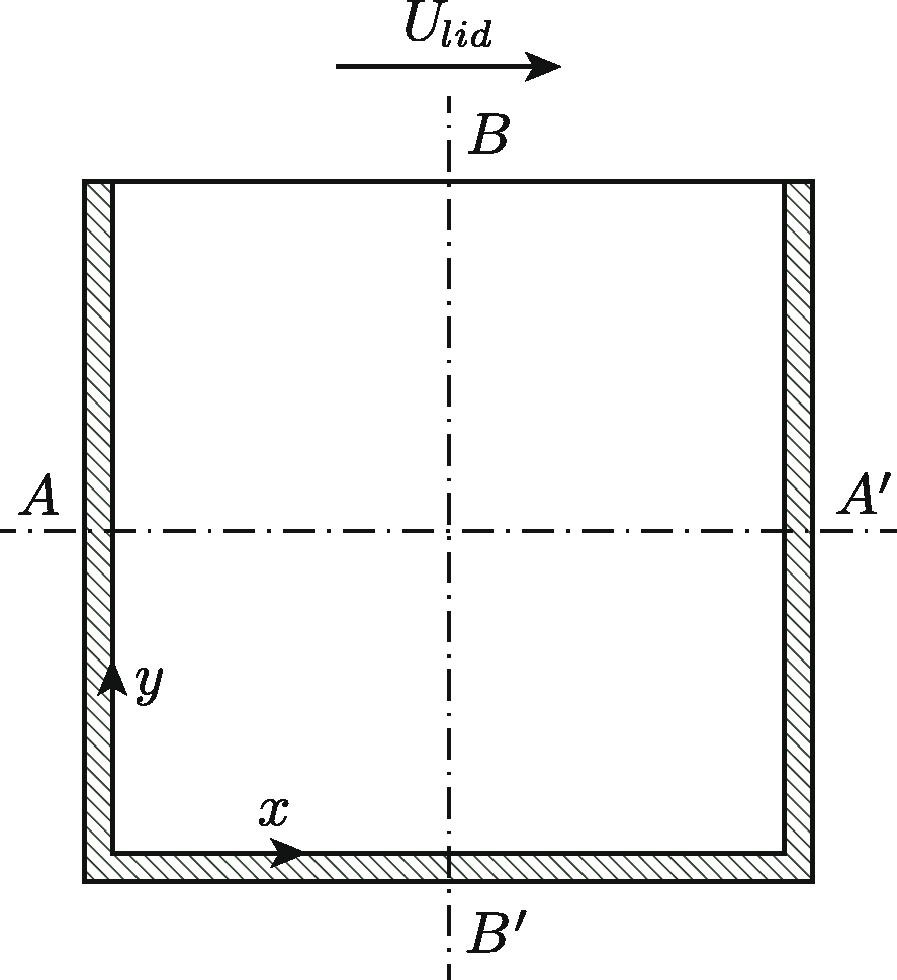
\includegraphics[width=.6\columnwidth]{geometry}
	\caption{2m$\times$2m 2D domain of the CNRS Benchmark. $U_{lid}$
	represents the velocity along the top boundary. Various quantities are
	measured along the centerlines AA' and BB' for comparison. From Tiberga et
	al. \cite{tiberga_results_2020}.}
	\label{fig:geometry}
\end{figure}

As shown in Figure \ref{fig:geometry}, the domain geometry is a 2m$\times$2m
square cavity filled with LiF-BeF$_2$-UF$_4$ molten salt at an initial
temperature of 900K \cite{tiberga_results_2020}.
Standard vacuum boundary conditions apply for neutron flux along all
boundaries whereby outgoing neutrons are considered lost, while homogeneous
boundary conditions apply for delayed neutron precursors. No-slip boundary
conditions apply for velocity variables in the cavity, except along the top
boundary for Steps 0.1, 0.3, 1.1, 1.2, and 1.4 which impose forced flow in the
form of lid-driven
cavity flow. For the temperature variable, all boundaries are insulated and we
simulate salt cooling with the following volumetric heat sink equation:
%
\begin{align}
    q'''(\vec{r}) &= \gamma \left(900 - T(\vec{r})\right) \label{eq:heat}
    \shortintertext{where}
    q''' &= \mbox{volumetric heat sink [W$\cdot$m$^{-3}$],}
    \nonumber \\
    \gamma &= \mbox{heat transfer coefficient [W$\cdot$m$^{-3}\cdot$K$^{-1}$],}
    \nonumber \\
    T(\vec{r}) &= \mbox{temperature at point $\vec{r}$ [K].} \nonumber
\end{align}

Tiberga et al. \cite{tiberga_results_2020} used Serpent 2
\cite{leppanen_serpent_2014} with the JEFF-3.1 library
\cite{koning_jeff-31_2006} to generate multigroup neutronics data for the
LiF-BeF$_2$-UF$_4$ salt in the domain at 900K, which they condensed into six
energy groups and eight precursor groups. We direct readers to their paper for
the group constant data \cite{tiberga_results_2020}. In addition, the
benchmark prescribes the following equations to govern the temperature
dependence in the cross sections and the neutron diffusion coefficients:
%
\begin{align}
    \Sigma_i (T) &= \Sigma_i(T_{ref})
    \frac{\rho_{fuel}(T)}{\rho_{fuel}(T_{ref})}
    \shortintertext{and}
    D (T) &= D(T_{ref})
    \frac{\rho_{fuel}(T_{ref})}{\rho_{fuel}(T)}
    \shortintertext{where}
    \Sigma_i &= \mbox{relevant macroscopic cross section [cm${-1}$],}
    \nonumber \\
    D &= \mbox{neutron diffusion coefficient [cm$^2\cdot$s$^{-1}$],}   
    \nonumber \\
    \rho_{fuel} &= \mbox{density of the fuel salt [kg$\cdot$m$^{-3}$],}
    \nonumber \\
    T_{ref} &= \mbox{reference temperature} = 900\mbox{ K}. \nonumber
\end{align}

The benchmark also prescribes incompressible Navier-Stokes flow with the
Boussinesq approximation for evaluating the salt flow in the
domain, but does not restrict the type of neutronics model.
The following subsections briefly detail each benchmark step, with Table
\ref{table:benchmark} listing the relevant input parameters and observables.

\begin{table*}[tp!]
	\caption{Input parameters and observables of each benchmark step.}
	\centering
	\footnotesize
	\begin{tabular}{p{.05\textwidth} p{.4\textwidth} p{.6\textwidth}}
		\toprule
		\textbf{Step} & \textbf{Input parameters} & \textbf{Observables} \\
		\midrule
		0.1 &
		\begin{itemize}[nosep,noitemsep,left=0pt,
		                before={\begin{minipage}[t]{\hsize}},
                        after ={\end{minipage}}]
		    \item $U_{lid} = 0.5$ m$\cdot$s$^{-1}$
		\end{itemize}\vspace*{-\baselineskip}\mbox{} &
		\begin{itemize}[nosep,noitemsep,left=0pt,
		                before={\begin{minipage}[t]{\hsize}},
                        after ={\end{minipage}}]
		    \item Velocity components $(u_x,u_y)$ along AA' and BB'
		\end{itemize}\vspace*{-\baselineskip}\mbox{} \\
        \midrule
        0.2 &
        \begin{itemize}[nosep,noitemsep,left=0pt,
		                before={\begin{minipage}[t]{\hsize}},
                        after ={\end{minipage}}]
		    \item $U_{lid} = 0$ m$\cdot$s$^{-1}$
		    \item $T = 900$ K
		    \item $P = 1$ GW
		\end{itemize} &
		\begin{itemize}[nosep,noitemsep,left=0pt,
		                before={\begin{minipage}[t]{\hsize}},
                        after ={\end{minipage}}]
		    \item Fission rate density $\sum^6_g \Sigma_{f,g} \phi_g(\vec{r})$ along AA'
            \item Reactivity $\rho$
		\end{itemize}\vspace*{-\baselineskip}\mbox{} \\
        \midrule
        0.3 &
        \begin{itemize}[nosep,noitemsep,left=0pt,
		                before={\begin{minipage}[t]{\hsize}},
                        after ={\end{minipage}}]
		    \item Fixed flow field from Step 0.1 for
		    $U_{lid} = 0.5$ m$\cdot$s$^{-1}$
		    \item Fixed heat source distribution
		    $\sum^6_{g} \epsilon_g \Sigma_{f,g} \phi_g(\vec{r})$ from Step 0.2
		    \item $\gamma = 10^6$ W$\cdot$m$^{-3}\cdot$K$^{-1}$
		\end{itemize} &
		\begin{itemize}[nosep,noitemsep,left=0pt,
		                before={\begin{minipage}[t]{\hsize}},
                        after ={\end{minipage}}]
		    \item Temperature $T$ along AA' and BB'
		\end{itemize}\vspace*{-\baselineskip}\mbox{} \\
        \midrule
        1.1 &
        \begin{itemize}[nosep,noitemsep,left=0pt,
		                before={\begin{minipage}[t]{\hsize}},
                        after ={\end{minipage}}]
		    \item Fixed flow field from Step 0.1 for
		    $U_{lid} = 0.5$ m$\cdot$s$^{-1}$
		    \item $T = 900$ K
		    \item $P = 1$ GW
		\end{itemize} &
		\begin{itemize}[nosep,noitemsep,left=0pt,
		                before={\begin{minipage}[t]{\hsize}},
                        after ={\end{minipage}}]
		    \item Delayed neutron source $\sum^8_i \lambda_i C_i$ along AA' and BB'
		    \item Reactivity change between Step 1.1 and Step 0.2,
		    $\Delta \rho = \rho - \rho_{s_{0.2}}$
		\end{itemize}\vspace*{-\baselineskip}\mbox{} \\
        \midrule
        1.2 &
        \begin{itemize}[nosep,noitemsep,left=0pt,
		                before={\begin{minipage}[t]{\hsize}},
                        after ={\end{minipage}}]
		    \item Fixed flow field from Step 0.1 for
		    $U_{lid} = 0.5$ m$\cdot$s$^{-1}$
		    \item $P = 1$ GW
		    \item $\gamma = 10^6$ W$\cdot$m$^{-3}\cdot$K$^{-1}$
		\end{itemize}\vspace*{-\baselineskip}\mbox{} &
		\begin{itemize}[nosep,noitemsep,left=0pt,
		                before={\begin{minipage}[t]{\hsize}},
                        after ={\end{minipage}}]
		    \item Temperature $T$ along AA' and BB'
            \item Reactivity change between Step 1.2 and Step 1.1,
            $\Delta\rho = \rho - \rho_{s_{1.1}}$
            \item Change in fission rate density
            $\sum^6_g \Sigma_{f,g} \phi_g(\vec{r}) -
            \left[\sum^6_g \Sigma_{f,g} \phi_g(\vec{r})\right]_{s_{0.2}}$
		\end{itemize} \\
        \midrule
        1.3 &
        \begin{itemize}[nosep,noitemsep,left=0pt,
		                before={\begin{minipage}[t]{\hsize}},
                        after ={\end{minipage}}]
		    \item $P = 1$ GW
		    \item $U_{lid} = 0$ m$\cdot$s$^{-1}$
		    \item $\gamma = 10^6$ W$\cdot$m$^{-3}\cdot$K$^{-1}$
		\end{itemize}\vspace*{-\baselineskip}\mbox{} &
		\begin{itemize}[nosep,noitemsep,left=0pt,
		                before={\begin{minipage}[t]{\hsize}},
                        after ={\end{minipage}}]
		    \item Velocity components $(u_x, u_y)$ along AA' and BB'
            \item Temperature $T$ along AA' and BB'
            \item Delayed neutron source $\sum^8_i \lambda_i C_i$ along AA' and BB'
            \item Reactivity change from Step 0.2
        $\Delta\rho = \rho - \rho_{s_{0.2}}$
		\end{itemize} \\
        \midrule
        1.4 &
        \begin{itemize}[nosep,noitemsep,left=0pt,
		                before={\begin{minipage}[t]{\hsize}},
                        after ={\end{minipage}}]
		    \item $\gamma = 10^6$ W$\cdot$m$^{-3}\cdot$K$^{-1}$
		    \item $P$ variable in the range $[0,1]$ GW with a step of 0.2 GW
		    \item $U_{lid}$ variable in the range $[0,0.5]$ m$\cdot$s$^{-1}$
		    with a step of 0.1 m$\cdot$s$^{-1}$
		\end{itemize} &
		\begin{itemize}[nosep,noitemsep,left=0pt,
		                before={\begin{minipage}[t]{\hsize}},
                        after ={\end{minipage}}]
		    \item Reactivity change between Step 1.4 and Step 0.2,
		    $\Delta\rho = \rho - \rho_{s_{0.2}}$, for all permutations of $P$
		    and $U_{lid}$ values
		\end{itemize}\vspace*{-\baselineskip}\mbox{} \\
        \midrule
        2.1 &
        \begin{itemize}[nosep,noitemsep,left=0pt,
		                before={\begin{minipage}[t]{\hsize}},
                        after ={\end{minipage}}]
		    \item $\gamma = 10^6$ W$\cdot$m$^{-3}\cdot$K$^{-1}$
            \item Steady-state solution from Step 1.4 for $U_{lid} = 0.5$
        m$\cdot$s$^{-1}$ and $P = 1.0$ GW
		\end{itemize} &
		\begin{itemize}[nosep,noitemsep,left=0pt,
		                before={\begin{minipage}[t]{\hsize}},
                        after ={\end{minipage}}]
		    \item Power gain and shift as a function of the perturbation frequency
		\end{itemize}\vspace*{-\baselineskip}\mbox{} \\
		\bottomrule
	\end{tabular}
	\label{table:benchmark}
\end{table*}

\subsection{Phase 0: Single physics}

In this preliminary phase, the steady-state solutions of
individual physics are studied without any multiphysics coupling.

\subsubsection{Step 0.1: Velocity field}

This step investigates the steady-state incompressible flow distribution in the
domain from a lid-driven cavity flow by imposing a non-zero horizontal
velocity along the top boundary. In addition, this step provides a fixed
velocity field for Steps 0.3, 1.1, and 1.2.

\subsubsection{Step 0.2: Neutronics}

This step tests neutronics capabilities through a criticality eigenvalue
problem in a static, isothermal fuel configuration by solving for the fission
rate density and effective multiplication factor $k_{eff}$. This step also aims
to identify deviations in results attributable to differences in neutronics
models and approximations. The total power $P$ is fixed to normalize the
neutron fluxes. For neutronics models conforming to the six neutron energy
group structure provided by Tiberga et al. \cite{tiberga_results_2020},
fission rate density is calculated as:
%
\begin{align}
    \text{Fission rate density} =& \sum^6_g \Sigma_{f,g} \phi_g(\vec{r})
    \shortintertext{where}
    \Sigma_{f,g} =& \text{ macroscopic fission cross section for neutron}
    \nonumber \\
    &\text{ in group $g$,} \nonumber \\
    \phi_g =& \text{ neutron flux in group $g$.} \nonumber
\end{align}

\subsubsection{Step 0.3: Temperature}

This step assesses passive scalar transport capability for determining the
temperature distribution independently from
the fluid flow and neutronics problems by imposing fixed velocity and fission
heat source distributions from Steps 0.1 and 0.2, respectively. Similar to the
fission rate density, the heat source distribution in six-group neutronics
models is calculated as:
%
\begin{align}
    \text{Heat source distribution} =& \sum^6_{g} \epsilon_g \Sigma_{f,g}
    \phi_g(\vec{r})
    \shortintertext{where}
    \epsilon_g =& \text{ average fission energy released by neutrons}
    \nonumber \\
    &\text{ in group $g$.} \nonumber
\end{align}

\subsection{Phase 1: Steady-state coupling}

Phase 1 builds towards simulating a fully-coupled multiphysics steady-state
system by gradually introducing coupling between various physics present in
a fast-spectrum molten salt system. All simulations are solved as steady-state
criticality eigenvalue problems.

\subsubsection{Step 1.1: Circulating fuel}

This step investigates effects of fuel salt flow on the neutronics,
namely the reactivity loss from the movement of precursors. The delayed neutron
precursors are allowed to drift under the fixed velocity field from Step 0.1
while keeping the temperature $T$ fixed at 900 K. With eight precursor groups,
the delayed neutron source is calculated as:
%
\begin{align}
    \text{Delayed neutron source} =& \sum^8_i \lambda_i C_i
    \shortintertext{where}
    \lambda_i =& \text{ average decay constant of delayed neutron} \nonumber \\
    &\text{ precursors in precursor group $i$,} \nonumber \\
    C_i =& \text{ concentration of delayed neutron precursors in}
    \nonumber \\
    &\text{ precursor group $i$.} \nonumber
\end{align}

\subsubsection{Step 1.2: Power coupling}

This step assesses the capability to accurately reproduce the change in
neutron flux distribution due to the fuel density reactivity feedback between
the neutron fluxes and the temperature distribution. We solve for the
steady-state neutron flux and temperature distributions under the fixed
velocity field from Step 0.1 and a volumetric heat sink described by Equation
\ref{eq:heat}.

\subsubsection{Step 1.3: Buoyancy}

Building on the previous step, we replace the fixed velocity field with
buoyancy-driven flow arising from the temperature gradients for a fully-coupled
multiphysics problem without forced flow. Barring any major discrepancies in
the previous steps, this step assesses the capability to reproduce the correct
buoyancy-driven flow profile and the subsequent effects on the neutronics and
temperature distribution due to precursor drift and fuel density reactivity
feedback.

\subsubsection{Step 1.4: Full coupling}

This step introduces forced flow to the fully-coupled problem through the
non-zero $U_{lid}$ boundary
condition. Thus, this problem most closely represents a molten salt system with
1) flow driven by an external force, 2) buoyancy flow effects, 3) \gls{DNP}
drift, and 4) thermal feedback effects on the neutronics. We solve for the
$k_{eff}$ under a range of $U_{lid}$ and $P$ values given in Table
\ref{table:benchmark}.

\subsection{Phase 2: Time dependent coupling}

In this phase, the transient response of the fully coupled nonlinear system is
studied.

\subsubsection{Step 2.1: Forced convection transient}

Linear perturbation analyses are performed in this step by introducing periodic
perturbations to the heat transfer coefficient $\gamma$ and studying the gain
and phase shift of the response in the total power $P$. For the initial
conditions, the steady-state solution from Step 1.4 with
$U_{lid} = 0.5$ m$\cdot$s$^{-1}$ and $P = 1$ GW is used. This initial
configuration is made exactly critical by scaling the neutron source terms,
from fission and \gls{DNP} decay, by the inverse of the criticality eigenvalue
solution from Step 1.4.

$\gamma$ is uniformly perturbed according to small-amplitude sine waves given
as:
%
\begin{align}
    \gamma =& \gamma_0 \left[ 1 + 0.1\sin\left(2 \pi f \right) \right]
    \shortintertext{where}
    \gamma_0 =& 10^6 \mbox{ W$\cdot$m$^{-3}\cdot$K$^{-1}$}, \nonumber \\
    f \in& \left\lbrace 0.0125, 0.025, 0.05, 0.1, 0.2, 0.4, 0.8 \right\rbrace 
    \mbox{ Hz.} \nonumber
\end{align}

The benchmark defines power gain as:
%
\begin{align}
    \mbox{Power gain} =& \frac{\left(P_{max} - P_{avg}\right)/P_{avg}}{
    \left(\gamma_{max} - \gamma_{avg}\right)/\gamma_{avg}}
\end{align}
%
The subscripts denote the maximum and time-averaged values of $P$ and $\gamma$.

\FloatBarrier

\section{Moltres} \label{sec:moltres}

%% Contents
% General description of Moltres and MOOSE
% Group constant data required from SCALE/Serpent
% Neutronics description
% Thermal-hydraulics description

In this section, we describe the Moltres, the \gls{MSR} simulation tool, and
the specific modeling approach for simulating the benchmark cases in Moltres.

\subsection{Description of Moltres}

Moltres \citep{lindsay_introduction_2018} is an open-source, \gls{MOOSE}-based
``application'' designed for multiphysics simulations of \glspl{MSR}. The goal
of making Moltres open-source is to promote quality through transparency and
ease of peer review. The source code \citep{lindsay_moltres_2017} is available
on GitHub \citep{github_build_2017}. Moltres leverages on \texttt{git} for
version control, and integrated testing to protect existing capabilities while
concurrently supporting continued code development. Moltres depends on the
\gls{MOOSE} finite element framework for its meshing and parallel, nonlinear
NEWTON-based solver capabilities. Therefore,
Moltres by default has access to tight coupling methods with implicit
time-stepping. Users can also opt to decouple problems for loosely coupled
solves depending on their specific needs. Furthermore, applications within the
\gls{MOOSE} framework share the same programming
interfaces; this commonality simplifies the work required to tightly couple
different physics over a wide range of length and time scales. For \gls{MSR}
simulations in Moltres such as those in this paper, we coupled Moltres'
\gls{MSR} modeling capabilities with \gls{MOOSE}'s \textit{Navier-Stokes} and
\textit{Heat Conduction} physics modules \citep{peterson_overview_2017} for
general thermal-hydraulics modeling. Together with these physics modules,
Moltres solves the multigroup neutron diffusion equations, for an arbitrary
number of energy and precursor groups, and thermal-hydraulics equations
simultaneously on the same mesh.

In a previous work, \cite{lindsay_introduction_2018}
demonstrated Moltres' \gls{MSR} neutronics modeling capabilities with 1D salt
flow in 2D-axisymmetric and 3D models of the \gls{MSRE}. The neutron flux and
temperature distributions showed good qualitative agreement with legacy
\gls{MSRE} data albeit with some minor quantitative discrepancies due to
simplifications and assumptions in the reactor geometry. Moltres has
since undergone further development to support the looping of \gls{DNP} drift
back into the reactor core, coupling the aforementioned \gls{DNP} drift
to incompressible Navier-Stokes velocity flows, and a decay heat model to
simulate decay heat from fission products.

To perform neutronics calculations, Moltres requires homogenized group constant
data from dedicated high-fidelity neutronics software such as SCALE
\citep{dehart_reactor_2011} or Serpent 2 \citep{leppanen_serpent_2014}. Users
can run a Python script in Moltres' Github repository which automatically reads
user-provided SCALE or Serpent 2 output data files and creates
Moltres-compatible JSON or text files containing all required group constant
data. There are on-going efforts to produce a similar script for parsing OpenMC
output data.

Moltres solves for the neutron fluxes governed by
the multigroup neutron diffusion equations given by:
%
\begin{align}
    \frac{1}{v_g} \frac{\partial \phi_g}{\partial t} =& \nabla \cdot D_g
    \nabla \phi_g - \Sigma^r_g \phi_g +
    \sum^G_{g' \neq g} \Sigma^s_{g' \rightarrow g} \phi_{g'} \nonumber \\
    &+ \chi^p_g \sum^G_{g'=1} \left( 1-\beta \right) \nu \Sigma^f_{g'}
    \phi_{g'} + \chi^d_g \sum^I_i \lambda_i C_i, \label{eq:neut} \\
    %
    \intertext{where}
    v_g =& \text{ average speed of neutrons in group $g$ [cm$\cdot$s$^{-1}$],} 
    \nonumber \\
    \phi_g =& \text{ neutron flux in group $g$ [cm$^{-2}\cdot$s$^{-1}$],}
    \nonumber \\
    t =& \text{ time [s],} \nonumber \\
    D_g =& \text{ diffusion coefficient of neutrons in} \nonumber \\
    &\text{ group $g$ [cm$^2\cdot$s$^{-1}$],} \nonumber \\
    \Sigma^r_g =& \text{ macroscopic cross section for removal of} \nonumber \\
    &\text{ neutrons from group $g$ [cm$^{-1}$],} \nonumber \\
    \Sigma^s_{g' \rightarrow g} =& \text{ macroscopic cross section of
    scattering from} \nonumber \\
    &\text{ groups $g'$ to $g$ [cm$^{-1}$],} \nonumber \\
    \chi^p_g =& \text{ prompt fission spectrum for neutrons in} \nonumber \\
    &\text{ group $g$ [ - ],} \nonumber \\
    G =& \text{ total number of discrete neutron groups [ - ],} \nonumber \\
    \nu =& \text{ average number of neutrons produced per} \nonumber \\
    &\text{ fission [ - ],} \nonumber \\
    \Sigma^f_{g} =& \text{ macroscopic fission cross section for neutron}
    \nonumber \\
    &\text{ in group $g$ [cm$^{-1}$],} \nonumber \\
    \chi^d_g =& \text{ delayed fission spectrum for neutrons in} \nonumber \\
    &\text{ group $g$ [ - ],} \nonumber \\
    I =& \text{ total number of delayed neutron precursor} \nonumber \\
    &\text{ groups [ - ],} \nonumber \\
    \beta =& \text{ total delayed neutron fraction [ - ].} \nonumber
\end{align}

While Moltres is generally unit-agnostic, we use the CGS system here because
the length units for the neutron cross section data from SCALE and Serpent 2
are provided in centimeters. The delayed neutron precursor concentrations are
governed by the following equation:
%
\begin{align}
    \frac{\partial C_i}{\partial t} =& \beta_i \sum^G_{g'=1} \nu \Sigma^f_{g'}
    \phi_{g'} - \lambda_i C_i - \vec{u} \cdot \nabla C_i + \nabla \cdot
    D_{\text{P}} \nabla C_i, \label{eq:dnp} \\
    %
    \intertext{where}
    \beta_i =& \text{ delayed neutron fraction of precursor group $i$ [ - ],}
    \nonumber \\
    \lambda_i =& \text{ average decay constant of delayed neutron} \nonumber \\
    &\text{ precursors in precursor group $i$ [s$^{-1}$],} \nonumber \\
    C_i =& \text{ concentration of delayed neutron precursors in}
    \nonumber \\
    &\text{ precursor group $i$ [cm$^{-3}$],} \nonumber \\
    \vec{u} =& \text{ molten salt flow velocity vector [cm$\cdot$s$^{-1}$],}
    \nonumber \\
    D_{\text{P}} =& \text{ effective diffusion coefficient of the delayed}
    \nonumber \\
    &\text{ neutron precursors [cm$^2\cdot$s$^{-1}$].} \nonumber
\end{align}

The last two terms in Equation \ref{eq:dnp} represent the advection and
diffusion terms, respectively, to model the movement of \gls{DNP} in
liquid-fuel \glspl{MSR}.

The governing equation for temperature is an advection-diffusion equation with
a fission heat source term given by:
%
\begin{align}
    \rho c_{p} \frac{\partial T}{\partial t} =& - \rho c_p \vec{u}
    \cdot \nabla T + \nabla \cdot \left(k \nabla T \right) + Q_f
    \label{eq:temp} \\
    %
    \intertext{where}
    Q_f =& \sum^G_{g=1} \epsilon_g \Sigma_g^f \phi_g \nonumber \\
    =& \text{ fission heat source [W$\cdot$m$^{-3}\cdot$s$^{-1}$],} \nonumber
    \\
    \rho =& \text{ density of the molten salt [kg$\cdot$m$^{-3}$],}
    \nonumber \\
    c_p =& \text{ specific heat capacity of molten salt} \nonumber \\
    &\text{ [J$\cdot$kg$^{-1}\cdot$K$^{-1}$],} \nonumber \\
    T =& \text{ temperature of molten salt [K]} \nonumber \\
    k =& \text{ effective thermal conductivity of molten salt} \nonumber \\
    &\text{ [W$\cdot$m$^{-1}\cdot$K$^{-1}$].} \nonumber
\end{align}

Lastly, the governing equations for the incompressible Navier-Stokes flow are
given by:
%
\begin{align}
    \rho \frac{\partial \vec{u}}{\partial t} =&
    -\rho (\vec{u}
    \cdot \nabla) \vec{u} - \nabla p + \mu \nabla^2 \vec{u}
    + \rho \alpha \vec{g} \left(T - T_{\text{ref}} \right)
    \label{eq:momemtum} \\
    %
    \nabla \cdot \vec{u} =& 0
    \label{eq:divergence}
    \intertext{where}
    p =& \text{ pressure [Pa],} \nonumber \\
    \mu =& \text{ dynamic viscosity [Pa$\cdot$s],} \nonumber \\
    \alpha =& \text{ coefficient of thermal expansion [K$^{-1}$],} \nonumber \\
    \vec{g} =& \text{ gravitational force vector [N$\cdot$m$^{-3}$],} \nonumber
    \\
    T_{\text{ref}} =& \text{ reference temperature at which the nominal}
    \nonumber \\
    &\text{ density is provided [K].} \nonumber
    \nonumber
\end{align}

\gls{MOOSE}'s \textit{Navier-Stokes} module also provides stabilization methods
to eliminate numerical node-to-node oscillations commonly observed when
resolving advection-dominated flows using continuous Galerkin methods. We refer
readers to \cite{peterson_overview_2017} for details on the implementation of
these methods in \gls{MOOSE}'s Navier-Stokes module. Moltres handles all the
aforementioned partial differential equations via the continuous finite-element
treatment except for the \gls{DNP} equation which Moltres solves via the
discontinuous finite element method to avoid instabilities in the \gls{DNP}
distribution without the need for stabilization methods.

\subsection{Modeling approach}

For this work, we ran the benchmark cases on a uniformly-spaced mesh consisting
of 200 by 200 elements. Thus, the dimensions of each mesh element are 0.01m by
0.01m. We
approximated most of the relevant variables, i.e. neutron fluxes, velocity
components, pressure, and temperature, using first-order Lagrange shape
functions. The only exception is the precursor concentration variables, which
we approximated using zeroth-order monomial shape functions and solved using
\gls{DFEM}. We took the group constant data directly from
\cite{tiberga_results_2020} and rewrote it into the Moltres-compatible text
format without any other modifications.

As mentioned in Section \ref{sec:moltres}, \gls{MOOSE}'s \textit{Navier-Stokes}
and \textit{Heat Conduction} modules provide some of the capabilities for
modeling incompressible flow and heat transfer. In particular, we stabilized
the incompressible flow and temperature governing equations using the
streamline upwind Petrov-Galerkin and pressure-stabilizing Petrov-Galerkin
stabilization methods \citep{peterson_overview_2017} implemented in
\gls{MOOSE}. Without these stabilization techniques, we observed spurious
numerical oscillations in the velocity and temperature. These oscillations are
commonly reported when using finite element methods to solve
advection-dominated flow and lid-driven cavity problems with corner
singularities where different boundary conditions meet
\citep{kuhlmann_lid-driven_2018}.

We performed all simulations using the Preconditioned \gls{JFNK} solver from
the \gls{MOOSE} framework. The coupled steady-state problems in
\textit{Steps 1.3} and \textit{1.4} required loose coupling between neutronics
and thermal-hydraulics due to the unique problem setup involving an eigenvalue
problem for the neutron multiplication factor and a standard steady-state
problem in thermal-hydraulics simultaneously. All other multiphysics problems
in \textit{Steps} in \textit{Phases 1} and \textit{2} were fully coupled
within the same \gls{JFNK} solve.

For the time-dependent cases in \textit{Step 2.1}, we used a second-order
implicit Backward Differential Formula (BDF2) time-stepping scheme and fixed
the timestep sizes at 1/200 of the period of the corresponding driving
frequencies as shown in Table \ref{table:timestep}. The only exception is the
0.0125 Hz case as a timestep size of 0.4s required more than one hundred
nonlinear iterations to converge in each timestep. We assumed the systems
reached asymptotic behavior when the magnitudes of neighboring power peaks
differed by less than 0.001\% for at least ten wavelengths. Under this
assumption, the phase shift
measurements between neighboring waves always converged, within the precision
governed by the timestep sizes, before the magnitudes of the power peaks.

\begin{table}[htb!]
    \caption{Timestep sizes used for the time-dependent cases in
    \textit{Step 2}.}
	\centering
	\setlength\tabcolsep{2.5pt}
	\begin{tabular}{l S S S S S S S}
	    \toprule
	    Frequency [Hz] & 0.0125 & 0.025 & 0.05 & 0.1 & 0.2 & 0.4 & 0.8 \\
	    \midrule
	    Timestep size [s] & 0.2 & 0.2 & 0.1 & 0.05 & 0.025 & 0.0125 & 0.00625
	    \\
	    \bottomrule
	\end{tabular}
	\label{table:timestep}
\end{table}
\section{Results}

In this section, we compare the results from Moltres for each CNRS Benchmark
step to the results in the benchmark paper \cite{tiberga_results_2020}.
The software packages from \gls{CNRS} and \gls{TUD}
each report two sets of results arising from different angular discretizations
in their neutronics models for Steps 0.2, 1.1, 1.2, 1.3, 1.4, and 2.1. These
sets of results are labeled as CNRS-$SP_1$ and
CNRS-$SP_3$; and TUD-$S_2$ and TUD-$S_6$, respectively. The
authors performed code-to-code verification by sampling observable values at
201 equidistant points along the centerlines AA' and BB' and reporting the
discrepancy $\epsilon_c$ of each observable from each software
(indexed by $c$) for each measured observable $Q_c$ (not to be confused with
fission heat source $Q_f$), relative to the average of
that same observable $Q_{avg}$ from all participating software. Variables
$\epsilon_c$ and $Q_{avg}$ are calculated as:
%
\begin{align}
    \epsilon_c =& \sqrt{\frac{\sum^{N_p}_{i=1}\left[Q_c(\vec{r_i}) - Q_{avg}
    (\vec{r_i})\right]^2}{\sum^{N_p}_{i=1} Q^2_{avg}(\vec{r_i})}}
    \shortintertext{and}
    Q_{avg}(\vec{r_i}) =& \frac{1}{N_c} \sum^{N_c}_{c=1} Q_c(\vec{r_i})
    \shortintertext{where}
    Q_c(\vec{r_i}) =&
    \mbox{ value of observable $Q$ at location $\vec{r_i}$ from software $c$,}
    \nonumber \\
    N_p =& \mbox{ number of sampling points of quantity $Q$} = 201,
    \nonumber \\
    N_c =& \mbox{ number of participating software packages.} \nonumber
\end{align}

The average discrepancy $\epsilon$ over all software is calculated as:
%
\begin{align}
    \epsilon =& \frac{1}{N_c}\sum^{N_c}_{c=1} \epsilon_c
\end{align}

We adopted the averaged values $\epsilon$ and $Q_{avg}$ directly from the
reference work \cite{tiberga_results_2020} without including our results
in the calculations. We note that the benchmark does not provide a reference
solution and a significantly erroneous value from one of the software packages
could heavily skew the discrepancy values. Nevertheless, the benchmark paper
reports good agreement among their software packages.

For observables measured along the centerlines AA' and/or BB', Tables
\ref{table:disc0} and \ref{table:disc1} report the discrepancy $\epsilon_c$ of
each observable from Moltres relative to the average of the benchmark
participants $Q_{avg}$ alongside the average discrepancy $\epsilon$ of
the benchmark participants. We also reproduce corresponding plots
in the benchmark paper for every observable along AA' or BB' in Figures
\ref{fig:0.1}, \ref{fig:0.2}, \ref{fig:0.3}, \ref{fig:1.1}, \ref{fig:1.2},
\ref{fig:1.3}, and \ref{fig:2.1} for a qualitative comparison of the results
from Moltres and the benchmark participants. Given the significant overlap in
the plot curves, these figures omit results from CNRS-$SP_1$ and TUD-$S_2$ to
reduce cluttering. Readers may also refer to
\ref{appendix:tables} for tables of observable values at nine equidistant
points along AA' and BB' from Moltres and the benchmark participants. We
provide these tables for ease of review and a direct comparison to
corresponding data tables from \cite{tiberga_results_2020}. The full dataset
of all observable results used in this results analysis is
available at \cite{park_results_2021}. Lastly, Table
\ref{table:rho} reports all reactivity and change in reactivity results from
Steps 0.2, 1.1, 1.2, and 1.3.

\begin{figure}[h]
	\centering
    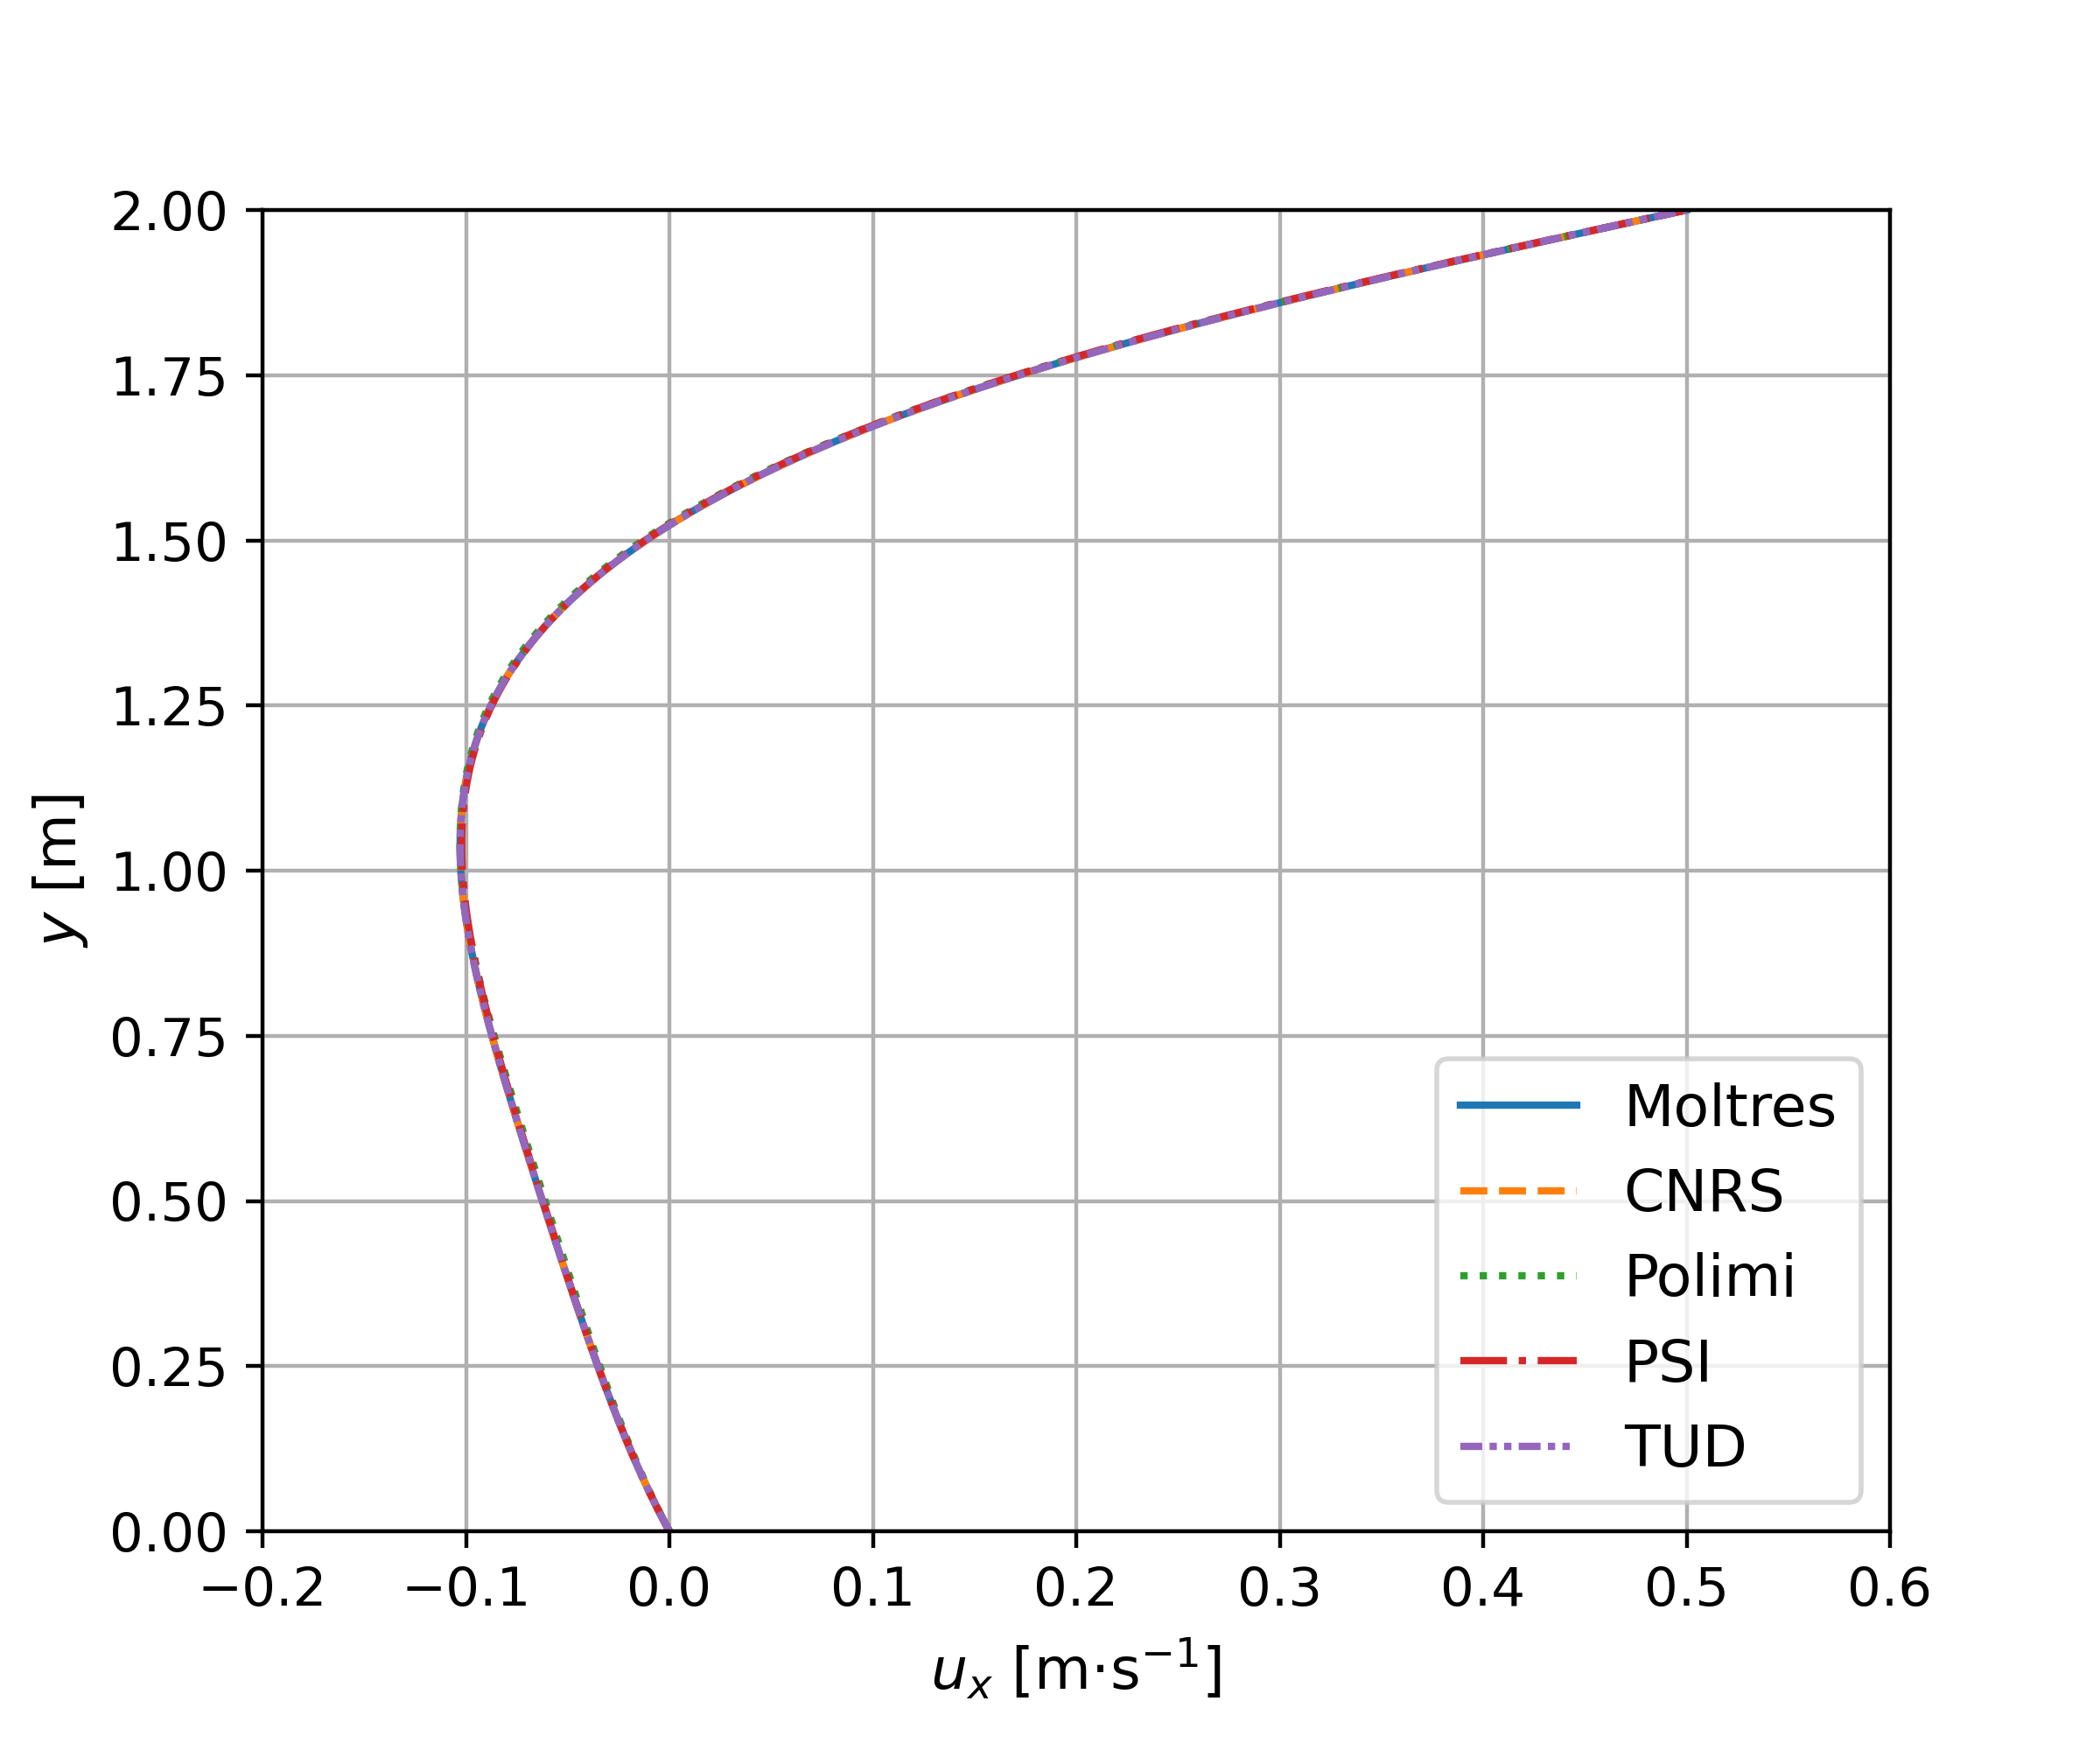
\includegraphics[width=.8\columnwidth]{0-1-vel-plot}
	\caption{Step 0.1 \textemdash\ Horizontal velocity component along BB'.}
	\label{fig:0.1}
\end{figure}
%
\begin{figure}[h]
	\centering
	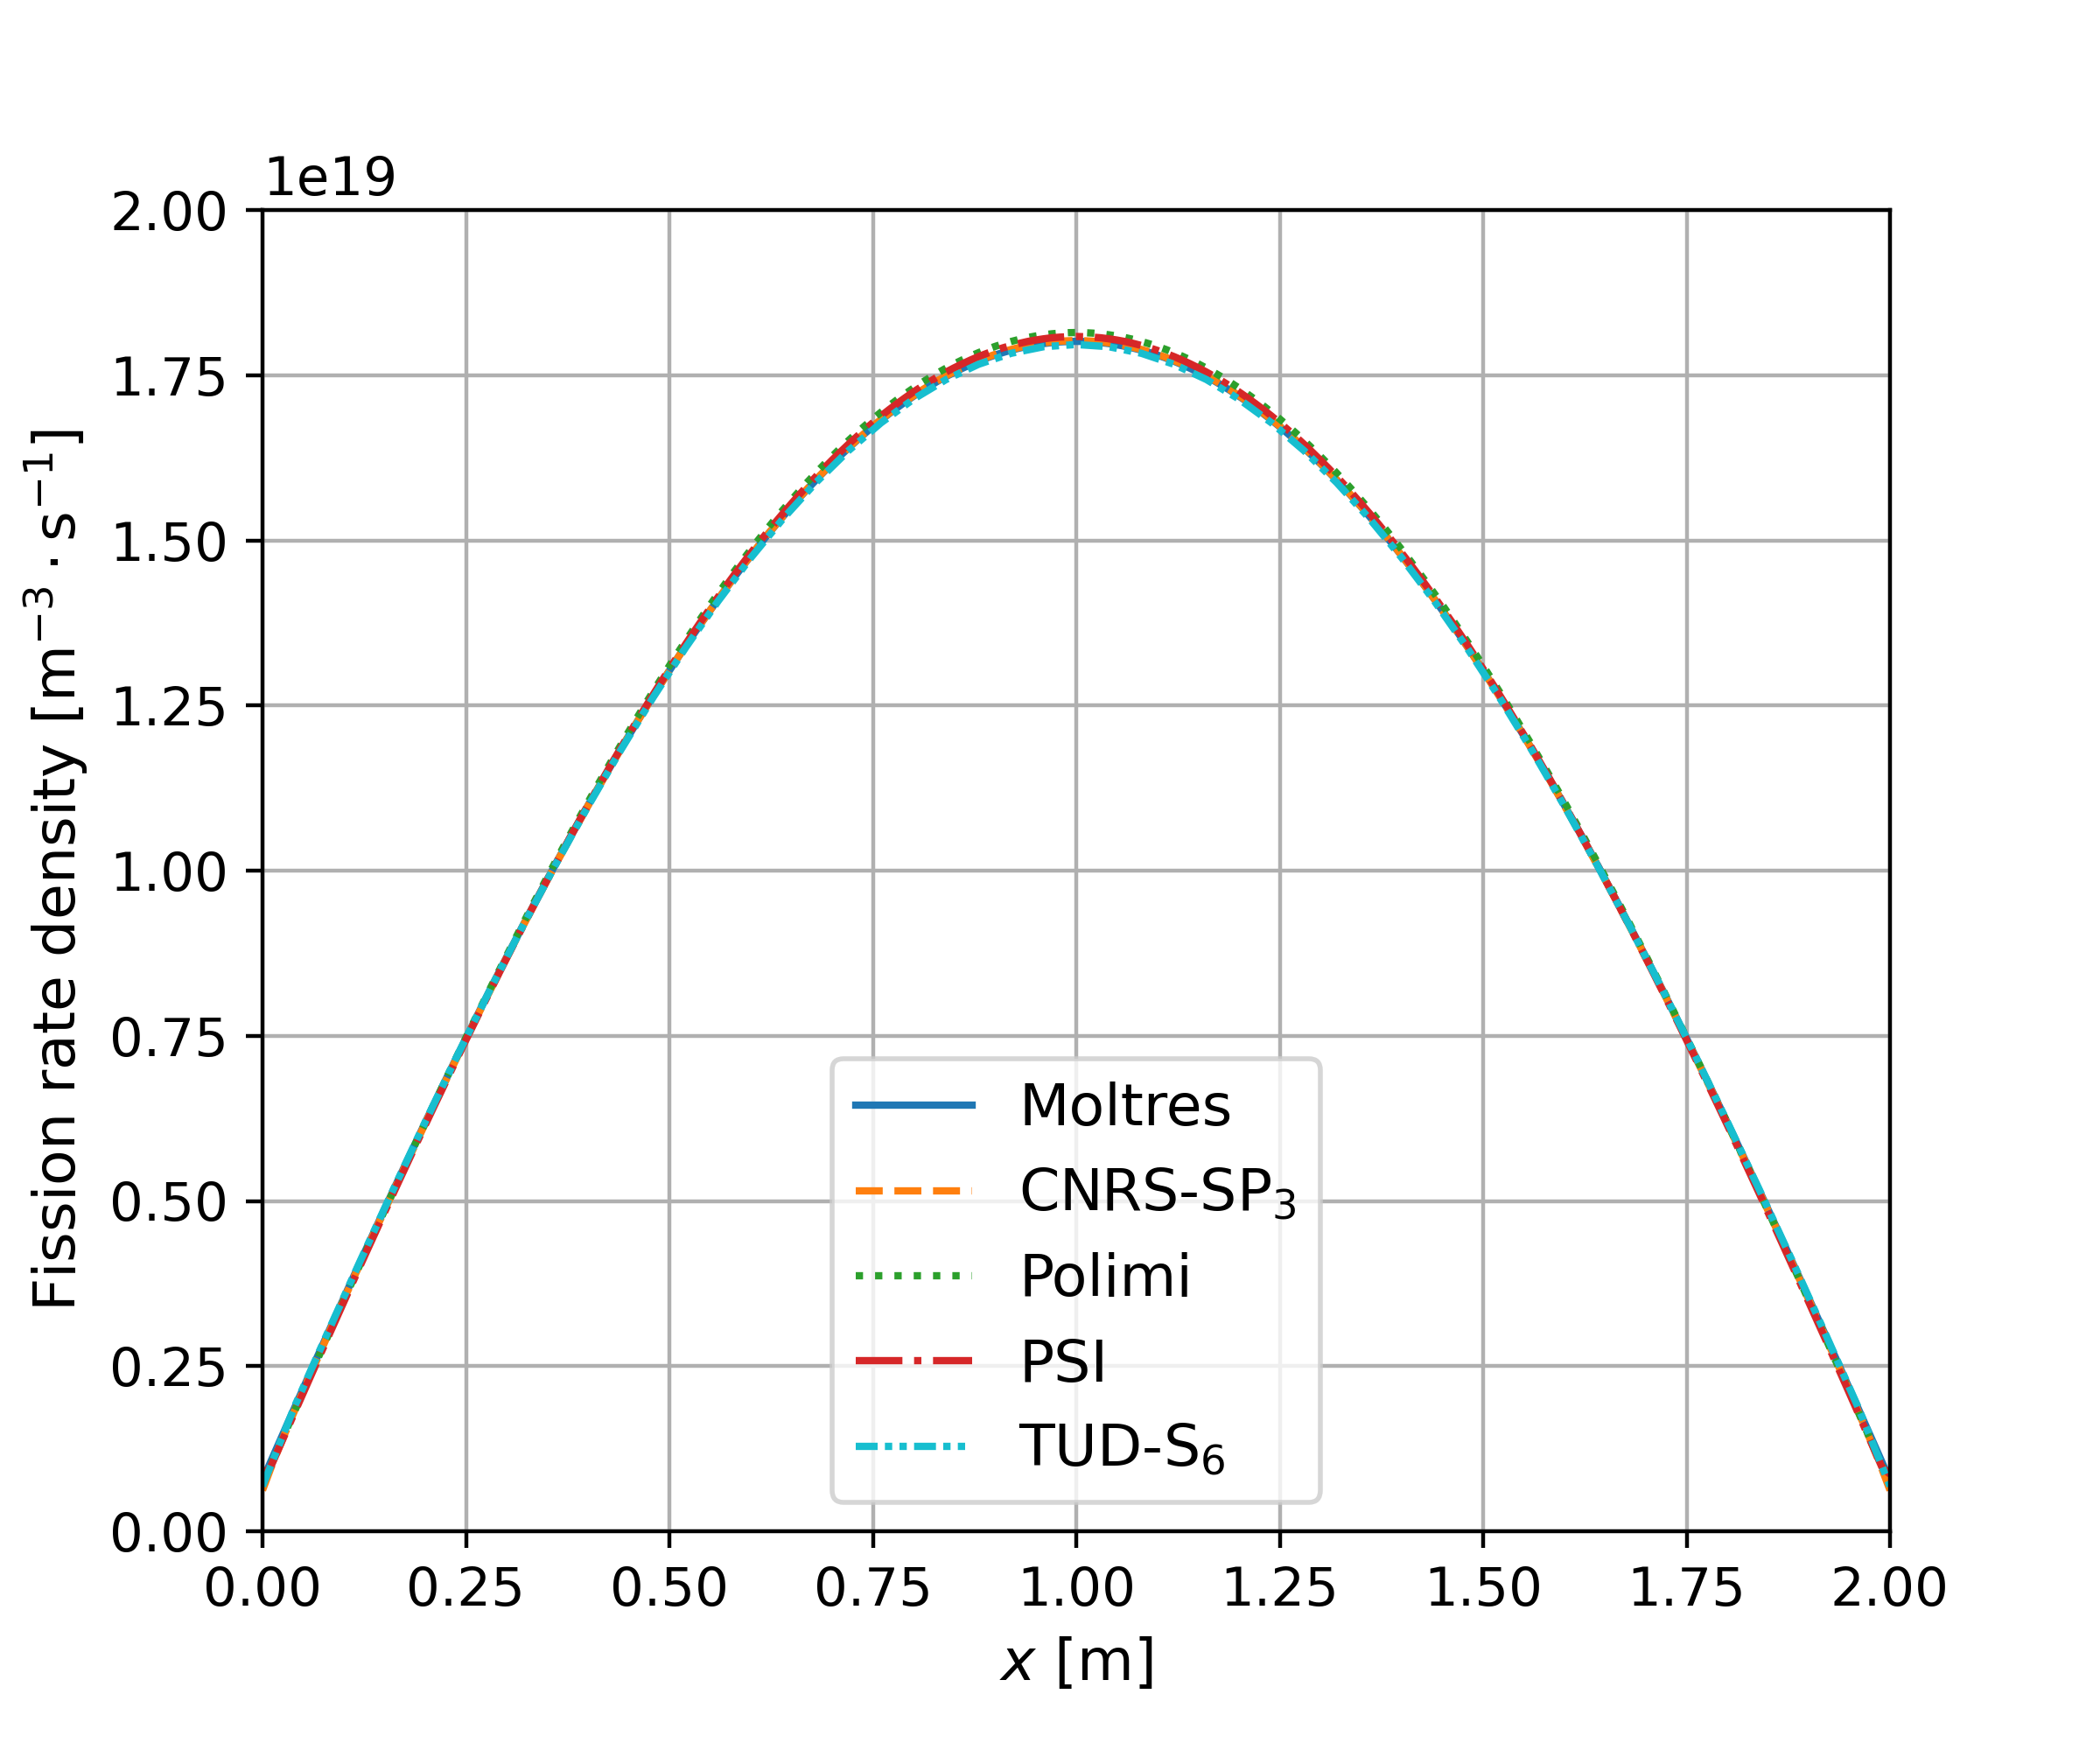
\includegraphics[width=.8\columnwidth]{0-2-fiss-plot}
	\caption{Step 0.2 \textemdash\ Fission rate density along AA'.}
	\label{fig:0.2}
	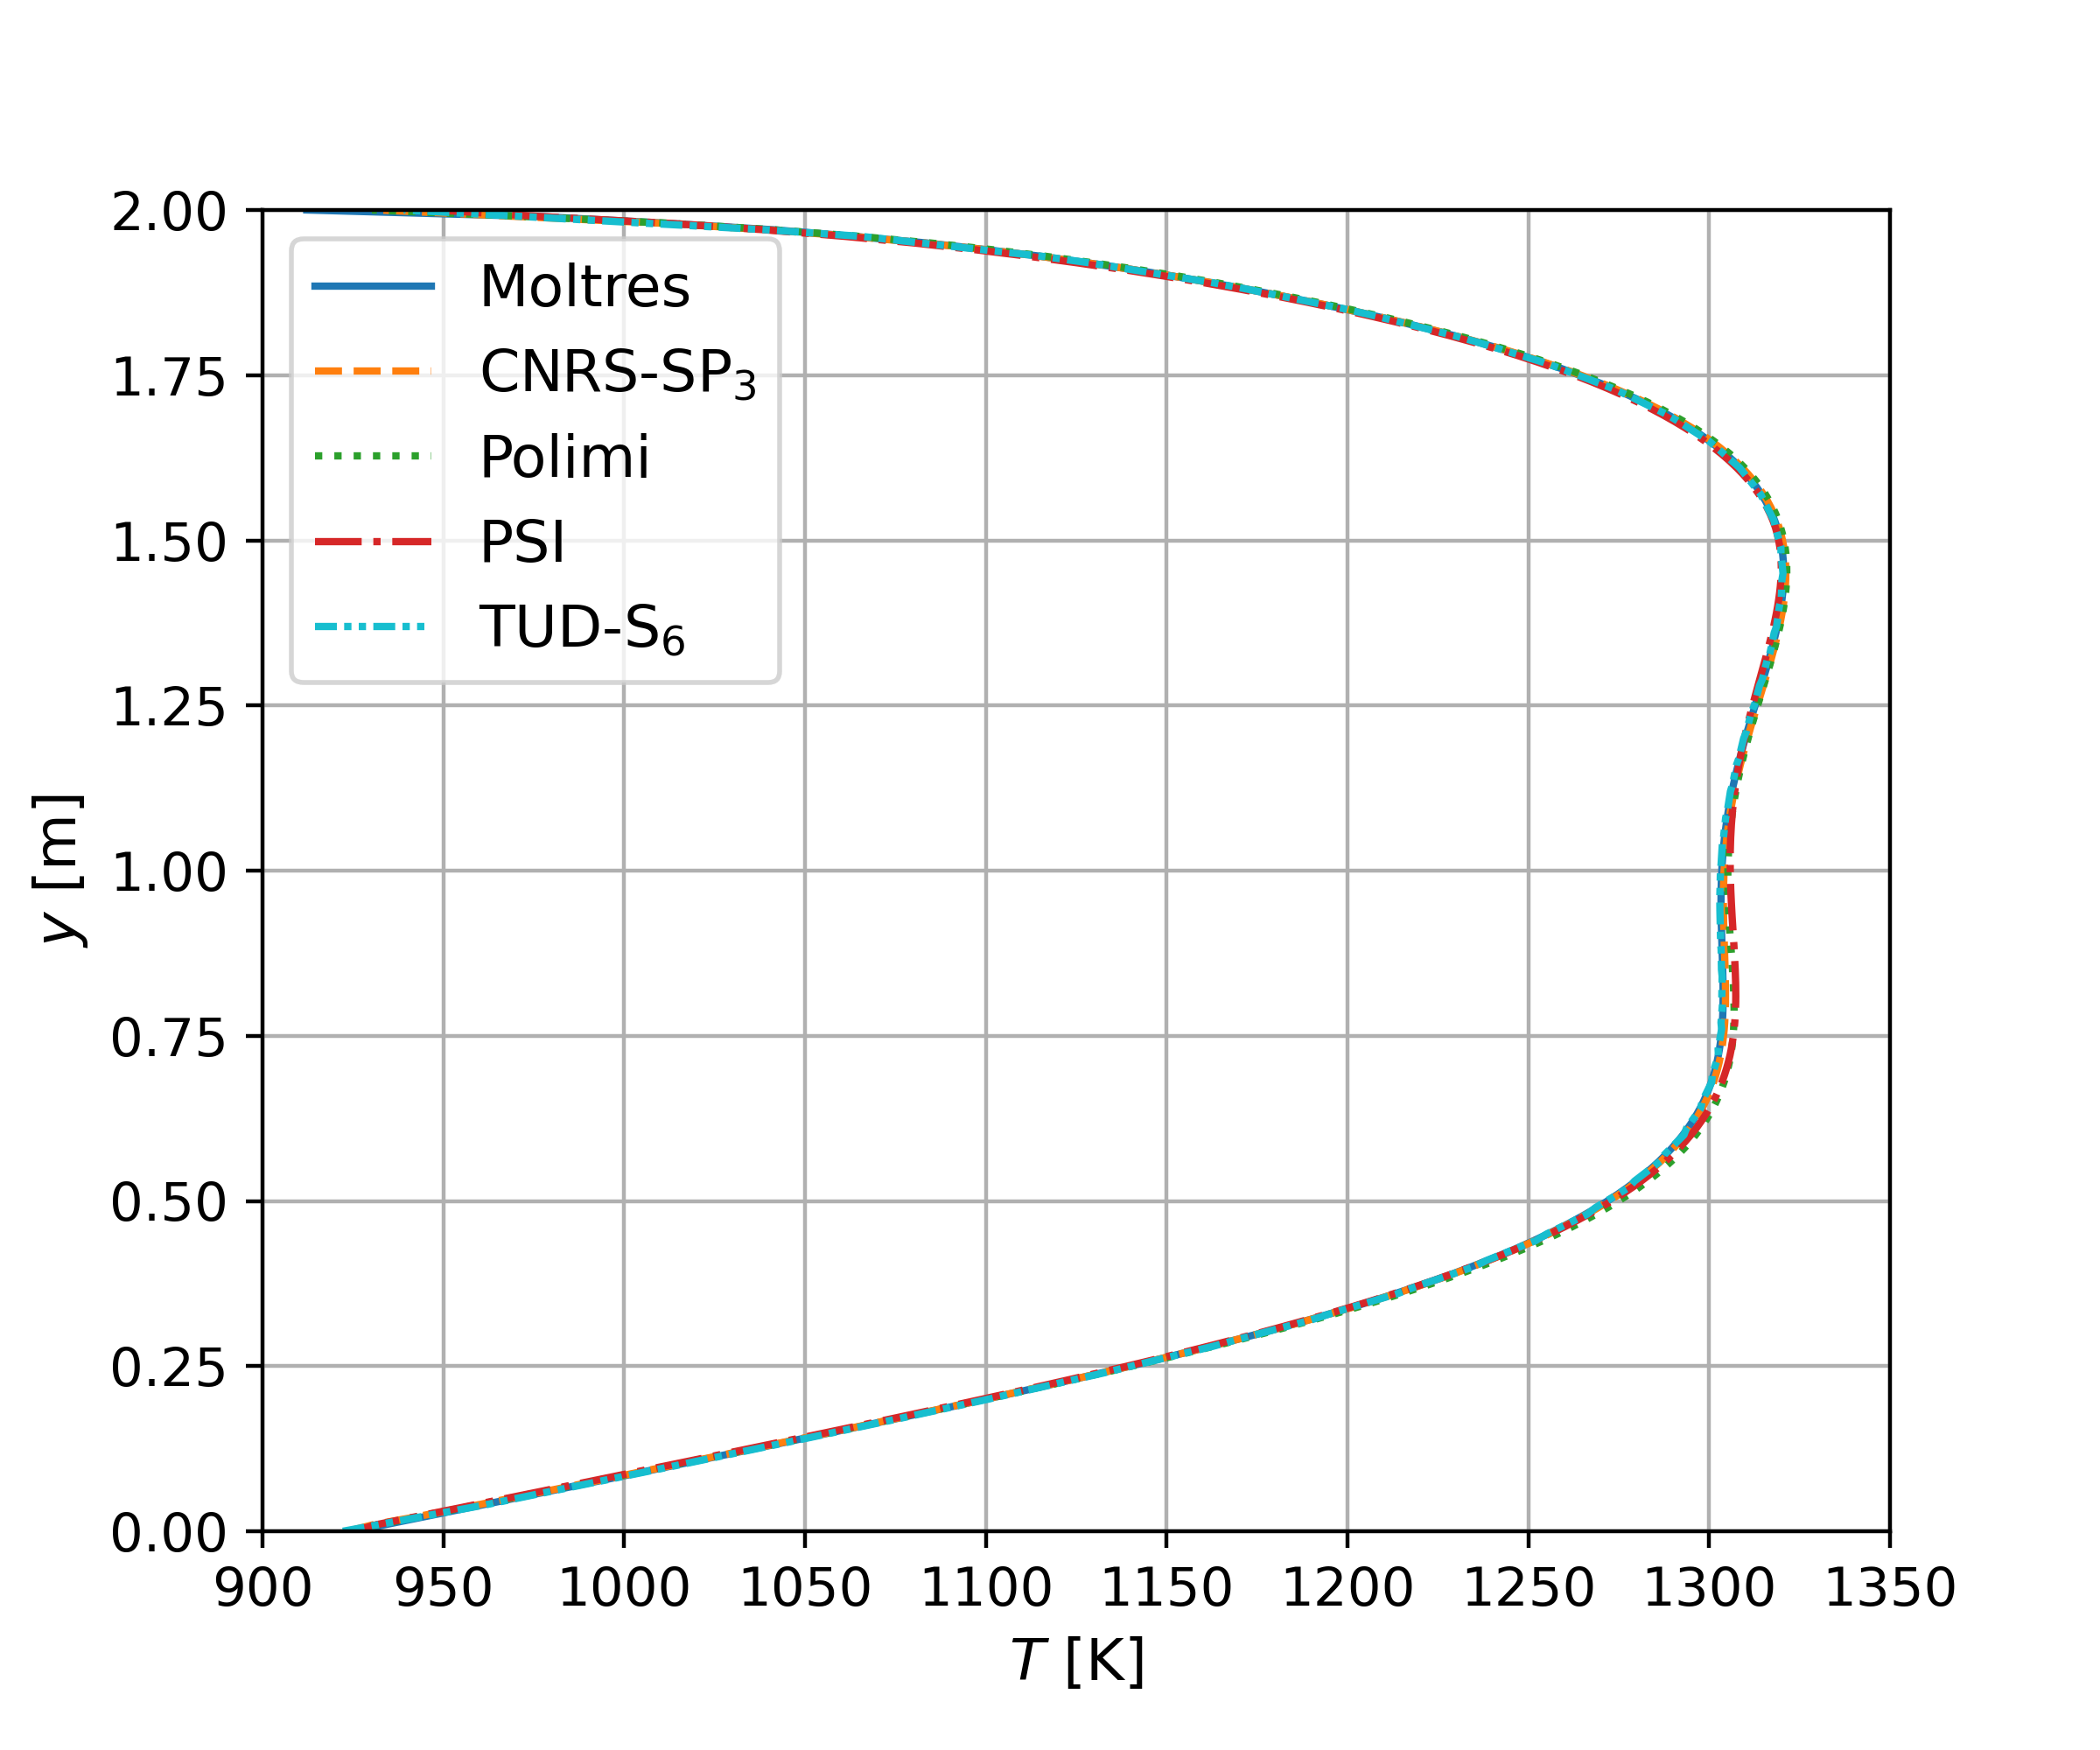
\includegraphics[width=.8\columnwidth]{0-3-temp-plot}
	\caption{Step 0.3 \textemdash\ Temperature distribution along BB'.}
	\label{fig:0.3}
\end{figure}
%
\FloatBarrier
%
\begin{table}[htb]
	\caption{Discrepancy values from Moltres alongside the average and standard
	deviation of the discrepancy values of the benchmark participants for Phase
	0.}
	\centering
	\small
	\begin{tabular}{l l c S S S}
		\toprule
		\multirow{2}{*}{\textbf{Step}} & \multirow{2}{*}{\textbf{Observable}} & \multirow{2}{*}{\textbf{Centerline}} & {\multirow{2}{*}{\textbf{Moltres [\%]}}} & \multicolumn{2}{c}{\textbf{Benchmark [\%]}} \\
		& & & & {Average} & {SD} \\
		\midrule
		\multirow{4}{*}{0.1} &
		\multirow{2}{*}{$u_x$} & AA' & 0.247 & 0.253 & 0.150 \\
		& & BB' & 0.266 & 0.318 & 0.102 \\
		\cmidrule{2-6}
		& \multirow{2}{*}{$u_y$} & AA' & 0.540 & 0.598 & 0.266 \\
		& & BB' & 0.468 & 0.795 & 0.421 \\
		\midrule
		{0.2} &
		{$\sum^6_g \Sigma_{f,g} \phi_g(\vec{r})$} & AA' & 0.313 & 0.285 & 0.153
		\\
		\midrule
		\multirow{2}{*}{0.3} &
		\multirow{2}{*}{$T$} & AA' & 0.090 & 0.085 & 0.031 \\
		& & BB' & 0.164 & 0.083 & 0.027\\
		\bottomrule
	\end{tabular}
	\label{table:disc0}
\end{table}

\subsection{Phase 0 results \& discussion}

Figures \ref{fig:0.1}, \ref{fig:0.2}, and \ref{fig:0.3} show that Moltres
accurately reproduced all three sets of results in Phase 0 for the velocity
field, fission rate density, and temperature. Table
\ref{table:disc0} reports the discrepancy values from Moltres for Phase 0 and
the corresponding average and \gls{SD} of the discrepancy values from
the benchmark participants
\cite{tiberga_results_2020}. Moltres performs very well as most discrepancy
values are either lower than or fall within one \gls{SD} of the benchmark
average discrepancies. The discrepancy value for $T$ along centerline BB' in
Step 0.3 is the only exception with its value of 0.164\% being larger than
the benchmark average by 3 \gls{SD}.

We
note in Figure \ref{fig:0.3} that the $T$ distribution from Moltres is almost
identical to the corresponding distributions from CNRS-$SP_3$ and TUD-$S_6$
along most of centerline BB'. However, Figure \ref{fig:0.3-zoom} shows
significant spread in the $T$ distributions along BB' from all software
packages near the top boundary. At $y = 2.0$ m, Moltres underpredicts the
temperature at 912.3 K compared to the benchmark participants' values which
range between 930.3 K and 948.1 K (Refer to Table \ref{table:0.3} for the
numerical values). This point on the top boundary lies directly downstream of
the velocity boundary condition discontinuity at the top-left corner.
Corner singularities are generally difficult to approximate with
continuous Galerkin methods \cite{kuhlmann_lid-driven_2018}.
The \gls{SUPG} stabilization scheme dampens numerical oscillations by
introducing pointwise artificial thermal diffusivity which depends strongly on
the inverse of local velocity magnitude \cite{peterson_overview_2018}.
Therefore, while the \gls{SUPG} scheme was very effective in eliminating
spurious numerical oscillations everywhere else, it provides little damping
along the top boundary due to the relatively large non-zero velocity boundary
condition. On the other hand, the temperature values in the rest of the domain
and the average discrepancies of the other variables show that Moltres can
still accurately reproduce the expected results and the temperature deviations
along the top boundary do not impact the overall integrity of our results.

\begin{figure}[htb]
	\centering
	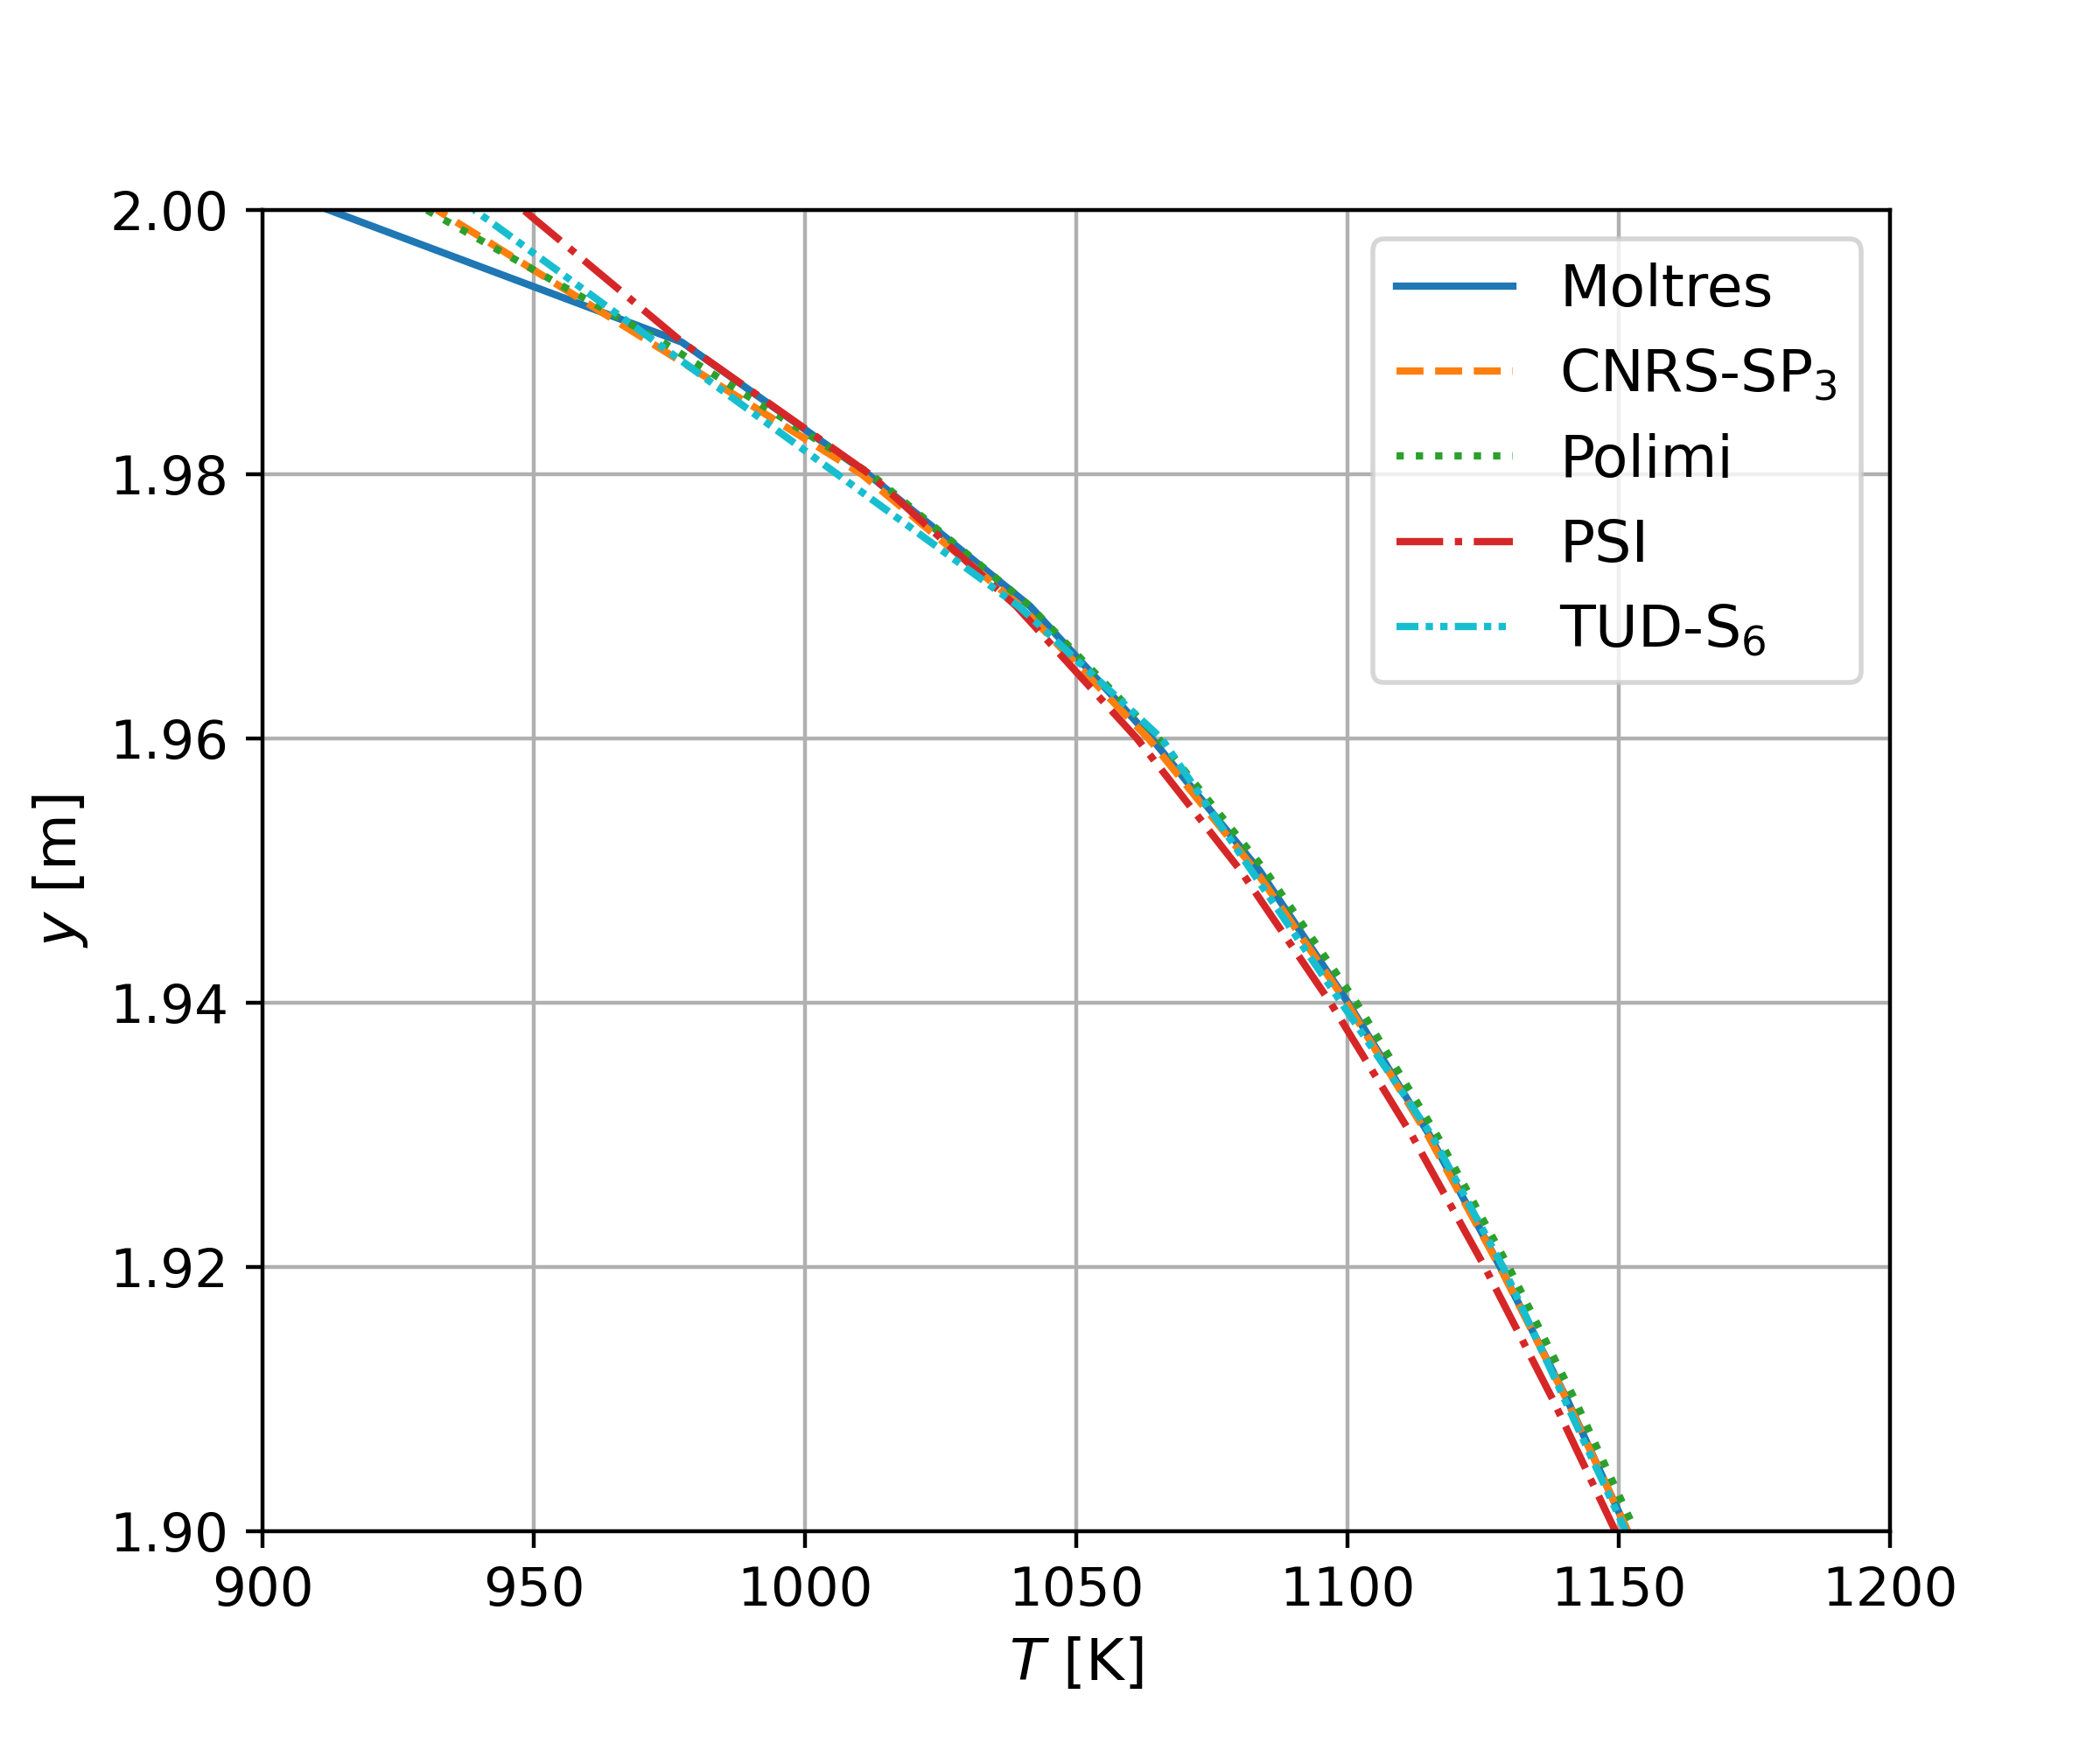
\includegraphics[width=.8\columnwidth]{0-3-temp-plot-zoom}
	\caption{Step 0.3 \textemdash\ Temperature distribution along BB' for y = 1.94 m to
	y = 2.00 m.}
	\label{fig:0.3-zoom}
\end{figure}

Lastly, we observe in table \ref{table:rho} that the reactivity $\rho$ value of
465.6 pcm from Moltres falls well within the range of $\rho$ values from the
benchmark which range from 353.7 pcm up to 578.1 pcm. Given that Moltres 
adopts the neutron diffusion model, our $\rho$ value agrees closest to the
results from the software packages which also adopt the neutron diffusion model
or theoretically-equivalent models such as the $SP_1$ and $S_2$ neutron
transport models, namely CNRS-$SP_1$, PoliMi, PSI, and TUD-$S_2$.

\begin{table}[htb]
    \caption{Reactivity $\rho$ and change in reactivity
    $\left(\rho_a - \rho_b\right)$ values from Steps 0.2, 1.1,
    1.2, and 1.3. All units are in pcm.}
    \centering
    \small
    \setlength\tabcolsep{2pt}
    \begin{tabular}{l S S S S}
        \toprule
        \multirow{2}{*}{\textbf{Software}} & {\textbf{Step 0.2}} &
        {\textbf{Step 1.1}} & {\textbf{Step 1.2}} & {\textbf{Step 1.3}} \\
        & {$\rho_{s_{0.2}}$}
        & {$\rho_{s_{1.1}} - \rho_{s_{0.2}}$}
        & {$\rho_{s_{1.2}} - \rho_{s_{1.1}}$}
        & {$\rho_{s_{1.3}} - \rho_{s_{0.2}}$} \\
        \midrule
        Moltres     & 465.6 & -62.7 & -1142.2 & -1207.7 \\
        CNRS-$SP_1$ & 411.3 & -62.5 & -1152.0 & -1220.5 \\
        CNRS-$SP_3$ & 353.7 & -62.6 & -1152.7 & -1220.7 \\
        PoliMi      & 421.2 & -62.0 & -1161.0 & -1227.0 \\
        PSI         & 411.7 & -63.0 & -1154.8 & -1219.6 \\
        TUD-$S_2$   & 482.6 & -62.0 & -1145.2 & -1208.5 \\
        TUD-$S_6$   & 578.1 & -60.7 & -1122.0 & -1184.4 \\
        \bottomrule
    \end{tabular}
    \label{table:rho}
\end{table}

\FloatBarrier

\subsection{Phase 1 results \& discussion}

Table \ref{table:disc1} shows the discrepancy values from Moltres relative to
the average and \gls{SD} of the benchmark participants for Steps 1.1, 1.2, and
1.3, and the corresponding average discrepancy values from the benchmark
\cite{tiberga_results_2020}. The subsequent subsections discuss the results
for each benchmark step in Phase 1.
%
\begin{table*}[htb]
	\caption{Discrepancy values from Moltres alongside the average and standard
	deviation of the discrepancy values of the benchmark participants for Phase
	1.}
	\centering
	\small
	\begin{tabular}{l l c S S S}
		\toprule
		\multirow{2}{*}{\textbf{Step}} & \multirow{2}{*}{\textbf{Observable}} & \multirow{2}{*}{\textbf{Centerline}} & {\multirow{2}{*}{\textbf{Moltres [\%]}}} & \multicolumn{2}{c}{\textbf{Benchmark [\%]}} \\
		& & & & {Average} & {SD} \\
		\midrule
		\multirow{2}{*}{1.1} &
		\multirow{2}{*}{$\sum_i \lambda_i C_i$} & AA' & 0.603 & 0.346 & 0.166
		\\
		& & BB' & 0.327 & 0.294 & 0.153 \\
		\midrule
		\multirow{4}{*}{1.2} &
		\multirow{2}{*}{$T$} & AA' & 0.076 & 0.095 & 0.015 \\
		& & BB' & 0.179 & 0.089 & 0.012 \\
		\cmidrule{2-6}
		& \multirow{2}{*}{\footnotesize $\Delta\left[\sum^6_g \Sigma_{f,g} \phi_g(\vec{r})
		\right]_{s_{1.2}-s_{0.2}}$} & AA' & 1.110 & 1.576 & 0.564 \\
		& & BB' & 1.089 & 1.133 & 0.392 \\
		\midrule
		\multirow{7}{*}{1.3} &
		{$u_x$} & AA' & 0.123 & 0.691 & 0.566 \\
		\cmidrule{2-6}
		& \multirow{2}{*}{$u_y$} & AA' & 0.237 & 0.329 & 0.131 \\
		& & BB' & 0.238 & 0.356 & 0.217 \\
		\cmidrule{2-6}
		& \multirow{2}{*}{$T$} & AA' & 0.064 & 0.057 & 0.023 \\
		& & BB' & 0.070 & 0.080 & 0.024 \\
		\cmidrule{2-6}
		& \multirow{2}{*}{$\sum_i \lambda_i C_i$} & AA' & 1.043 & 0.460 & 0.190
		\\
		& & BB' & 0.462 & 1.194 & 0.178 \\
		\bottomrule
	\end{tabular}
	\label{table:disc1}
\end{table*}

\subsubsection{Step 1.1: Circulating fuel}

Figure \ref{fig:1.1} shows good qualitative agreement in the delayed neutron
source distribution along BB' among Moltres and the benchmark participants.
From Table \ref{table:disc1}, Moltres reports discrepancies of 0.603\% and
0.327\% along the centerlines AA' and BB', respectively. Both values are on the
within two and one \gls{SD}, respectively, of the average discrepancies of the
benchmark participants (0.346\% and 0.294\%).
In Table \ref{table:rho}, we observe that the change in
$\rho$ relative to Step 0.2 is $-62.7$ pcm for Moltres and this value is
consistent with the $-63.0$ to $-62.0$ pcm range that most of the benchmark
participants' values fall in.
%
\begin{figure}[h!]
	\centering
    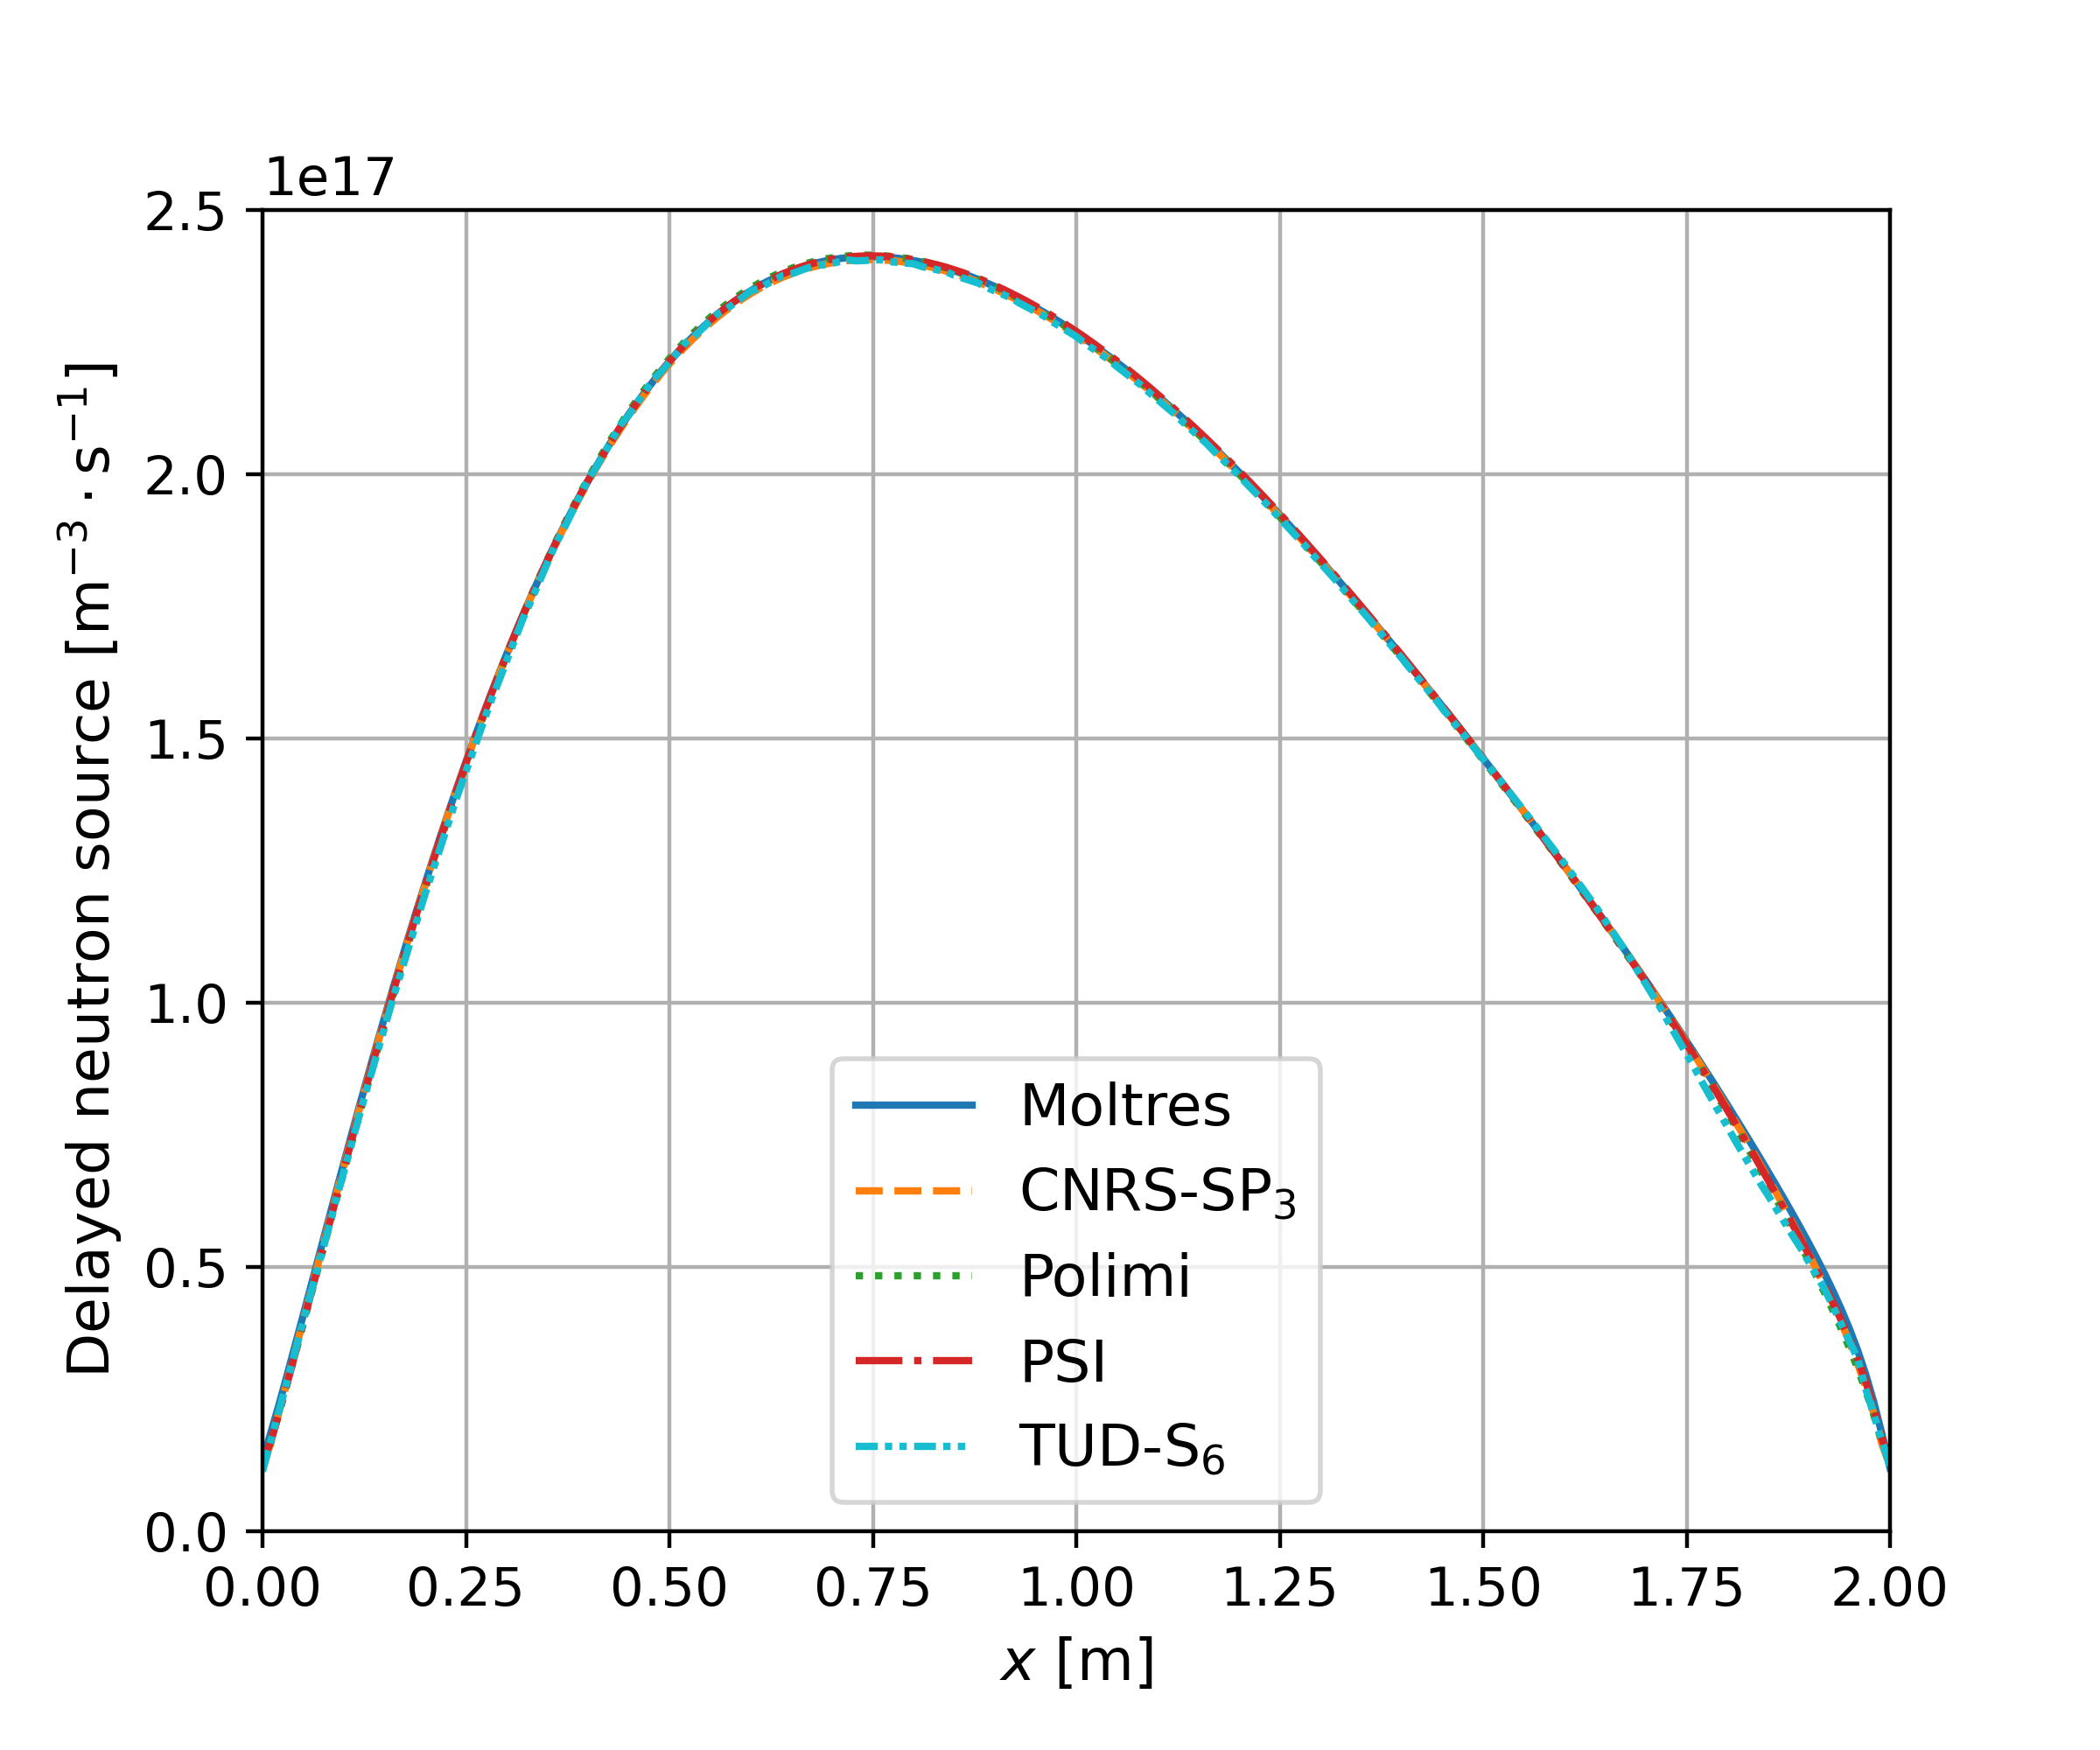
\includegraphics[width=.8\columnwidth]{1-1-dnp-x-plot}
    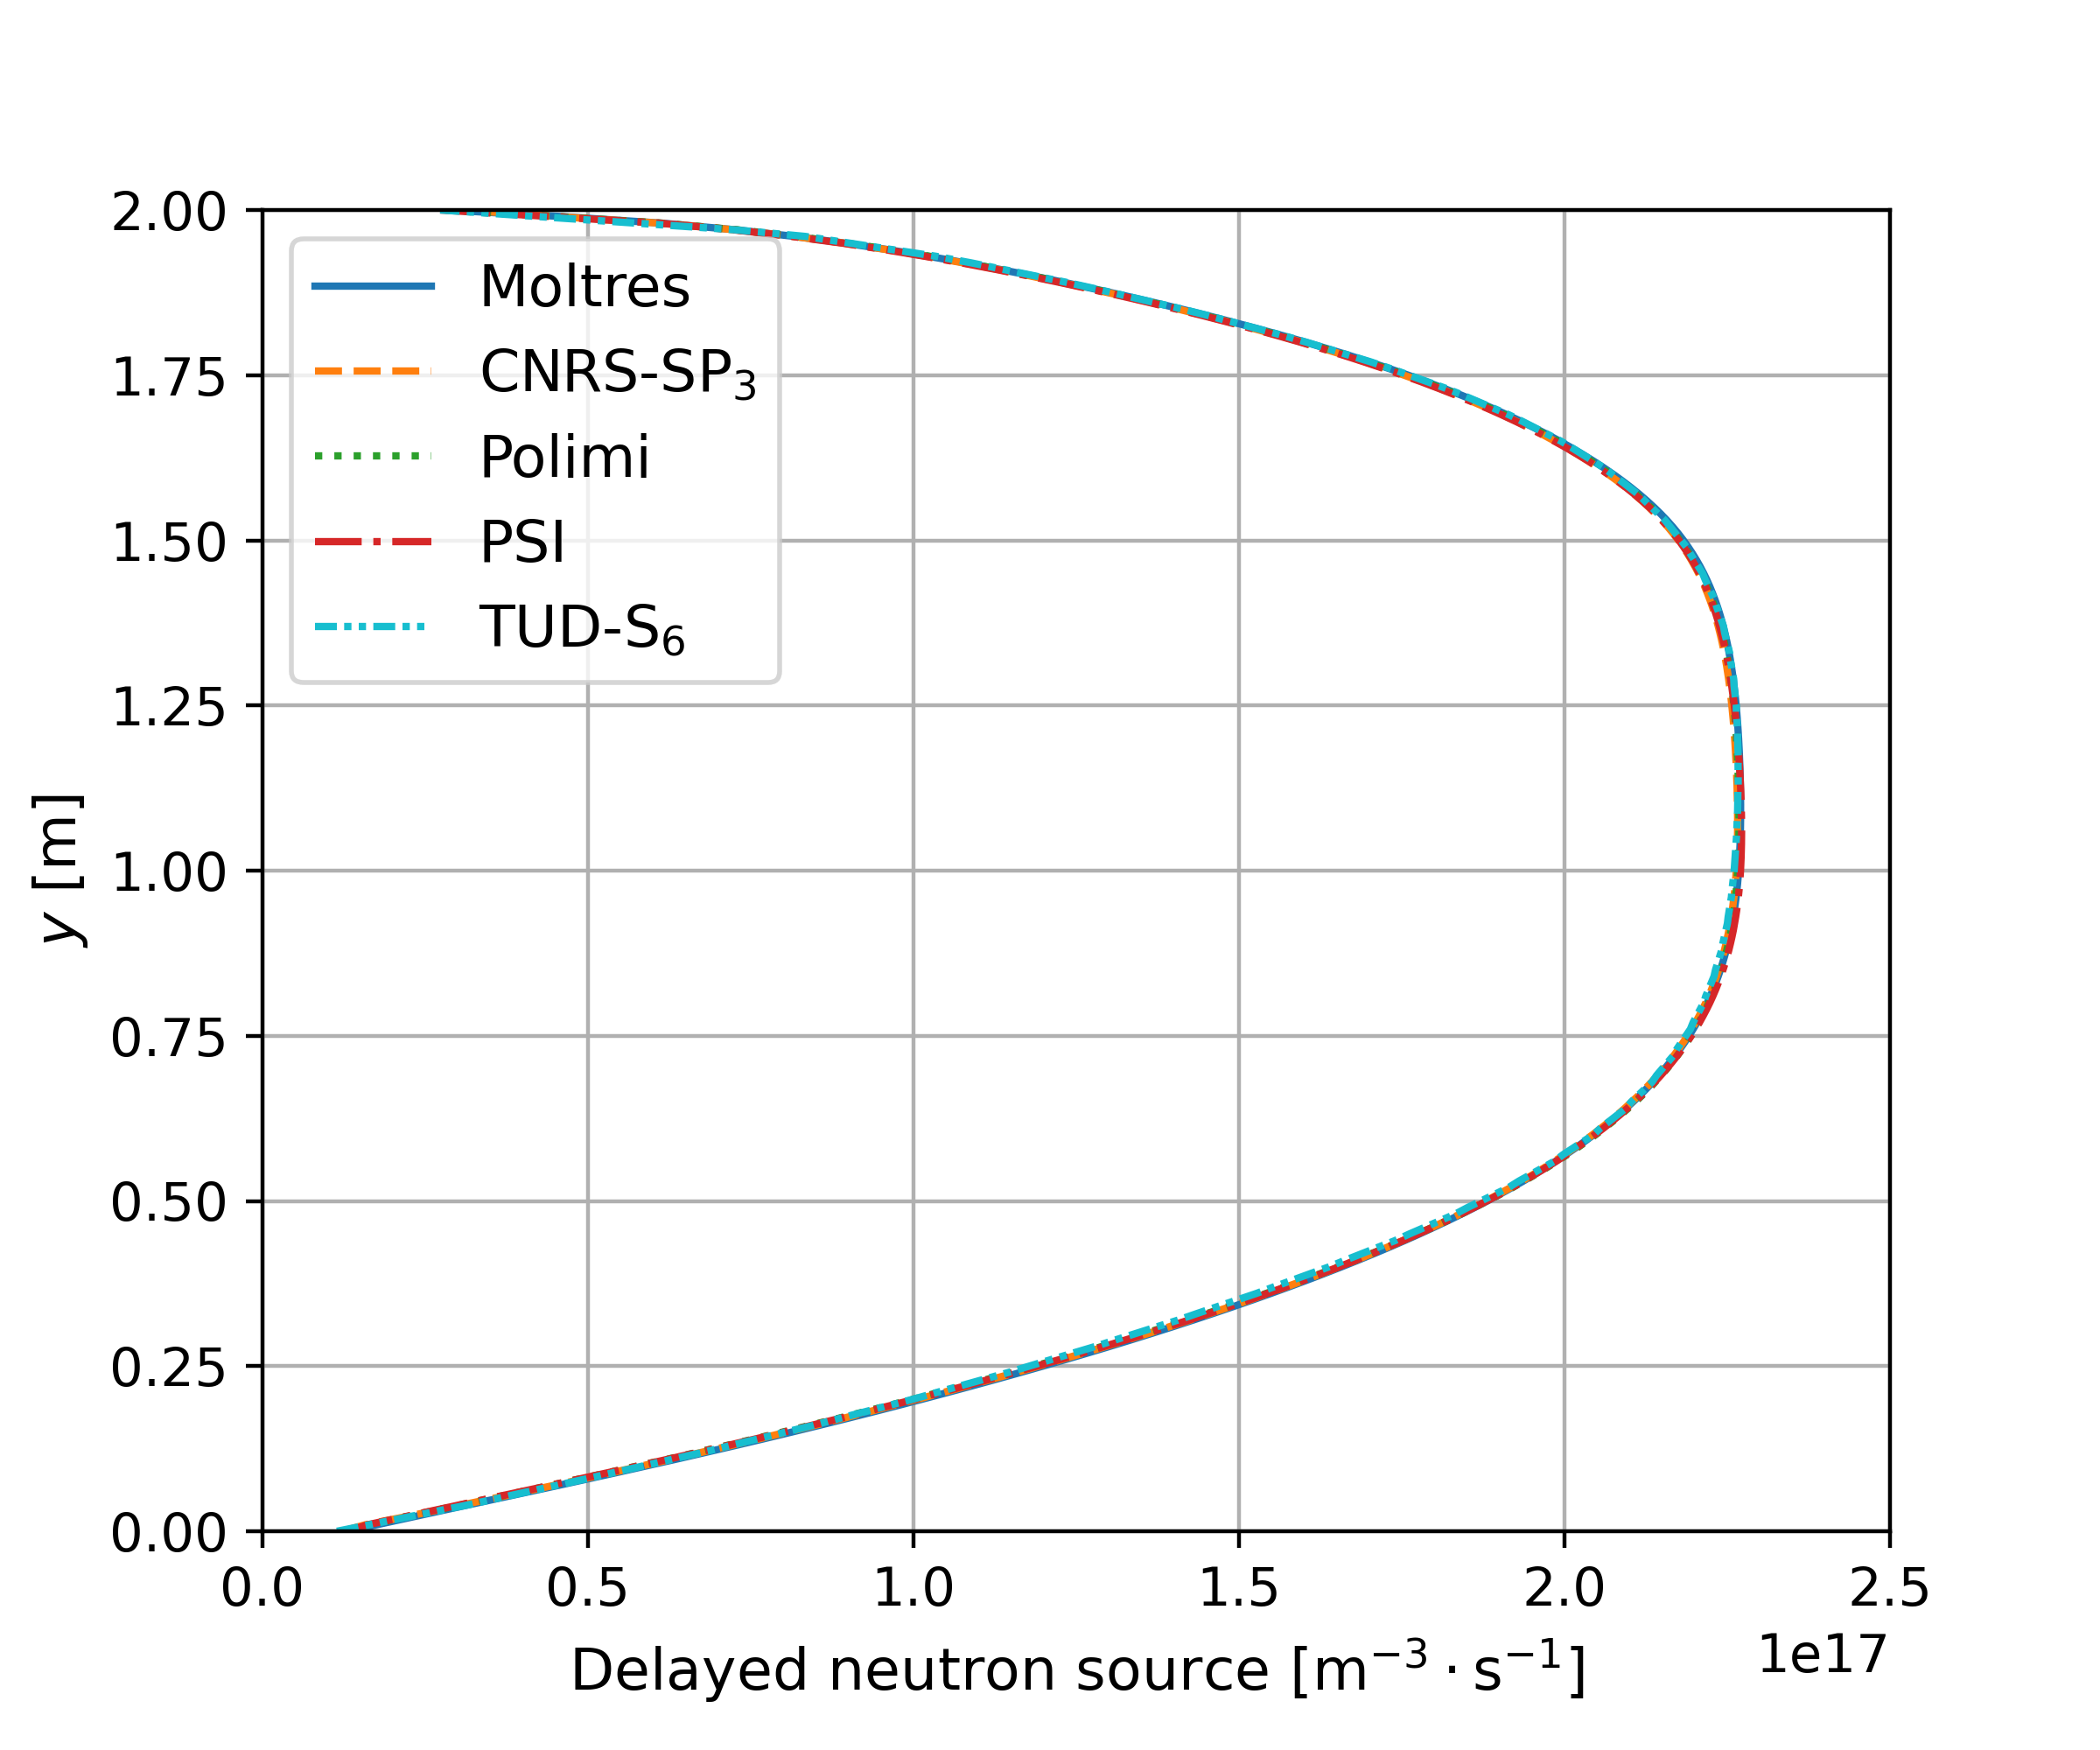
\includegraphics[width=.8\columnwidth]{1-1-dnp-y-plot}
	\caption{Step 1.1 \textemdash\ Delayed neutron source along AA' (top) and BB'
	(bottom).}
	\label{fig:1.1}
\end{figure}
%
\begin{figure*}[htb]
	\centering
	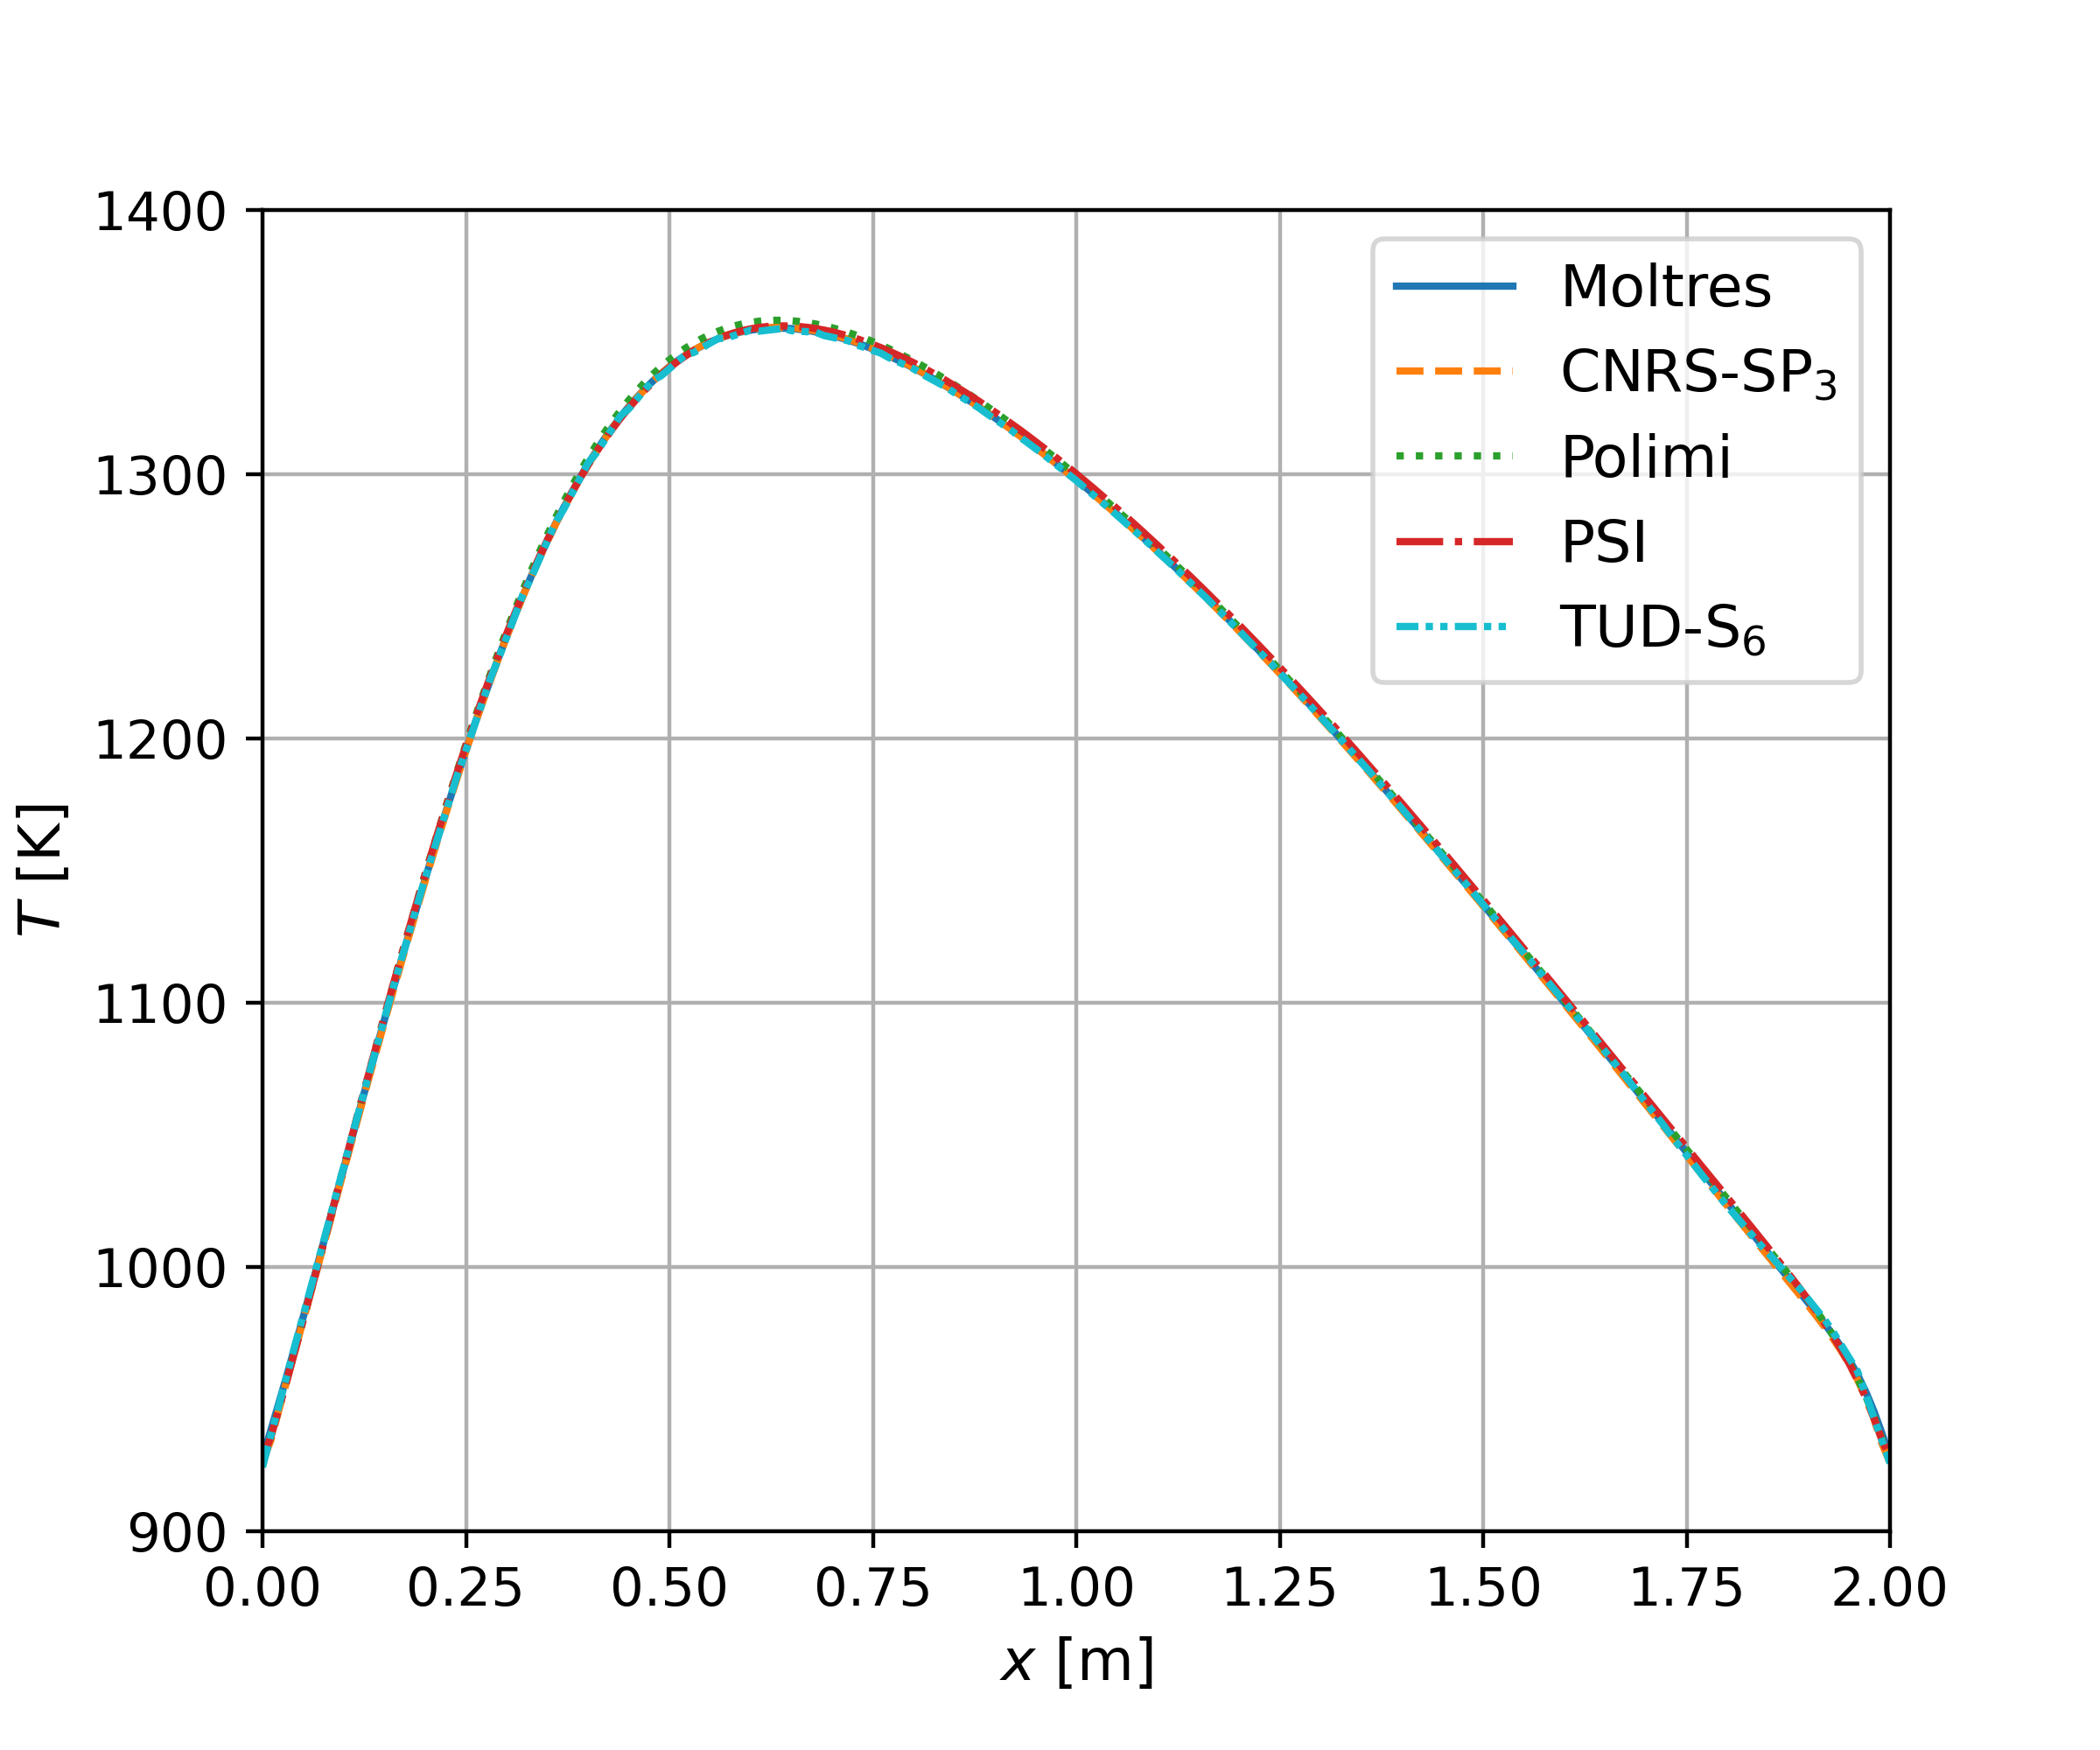
\includegraphics[width=.8\columnwidth]{1-2-temp-plot}
	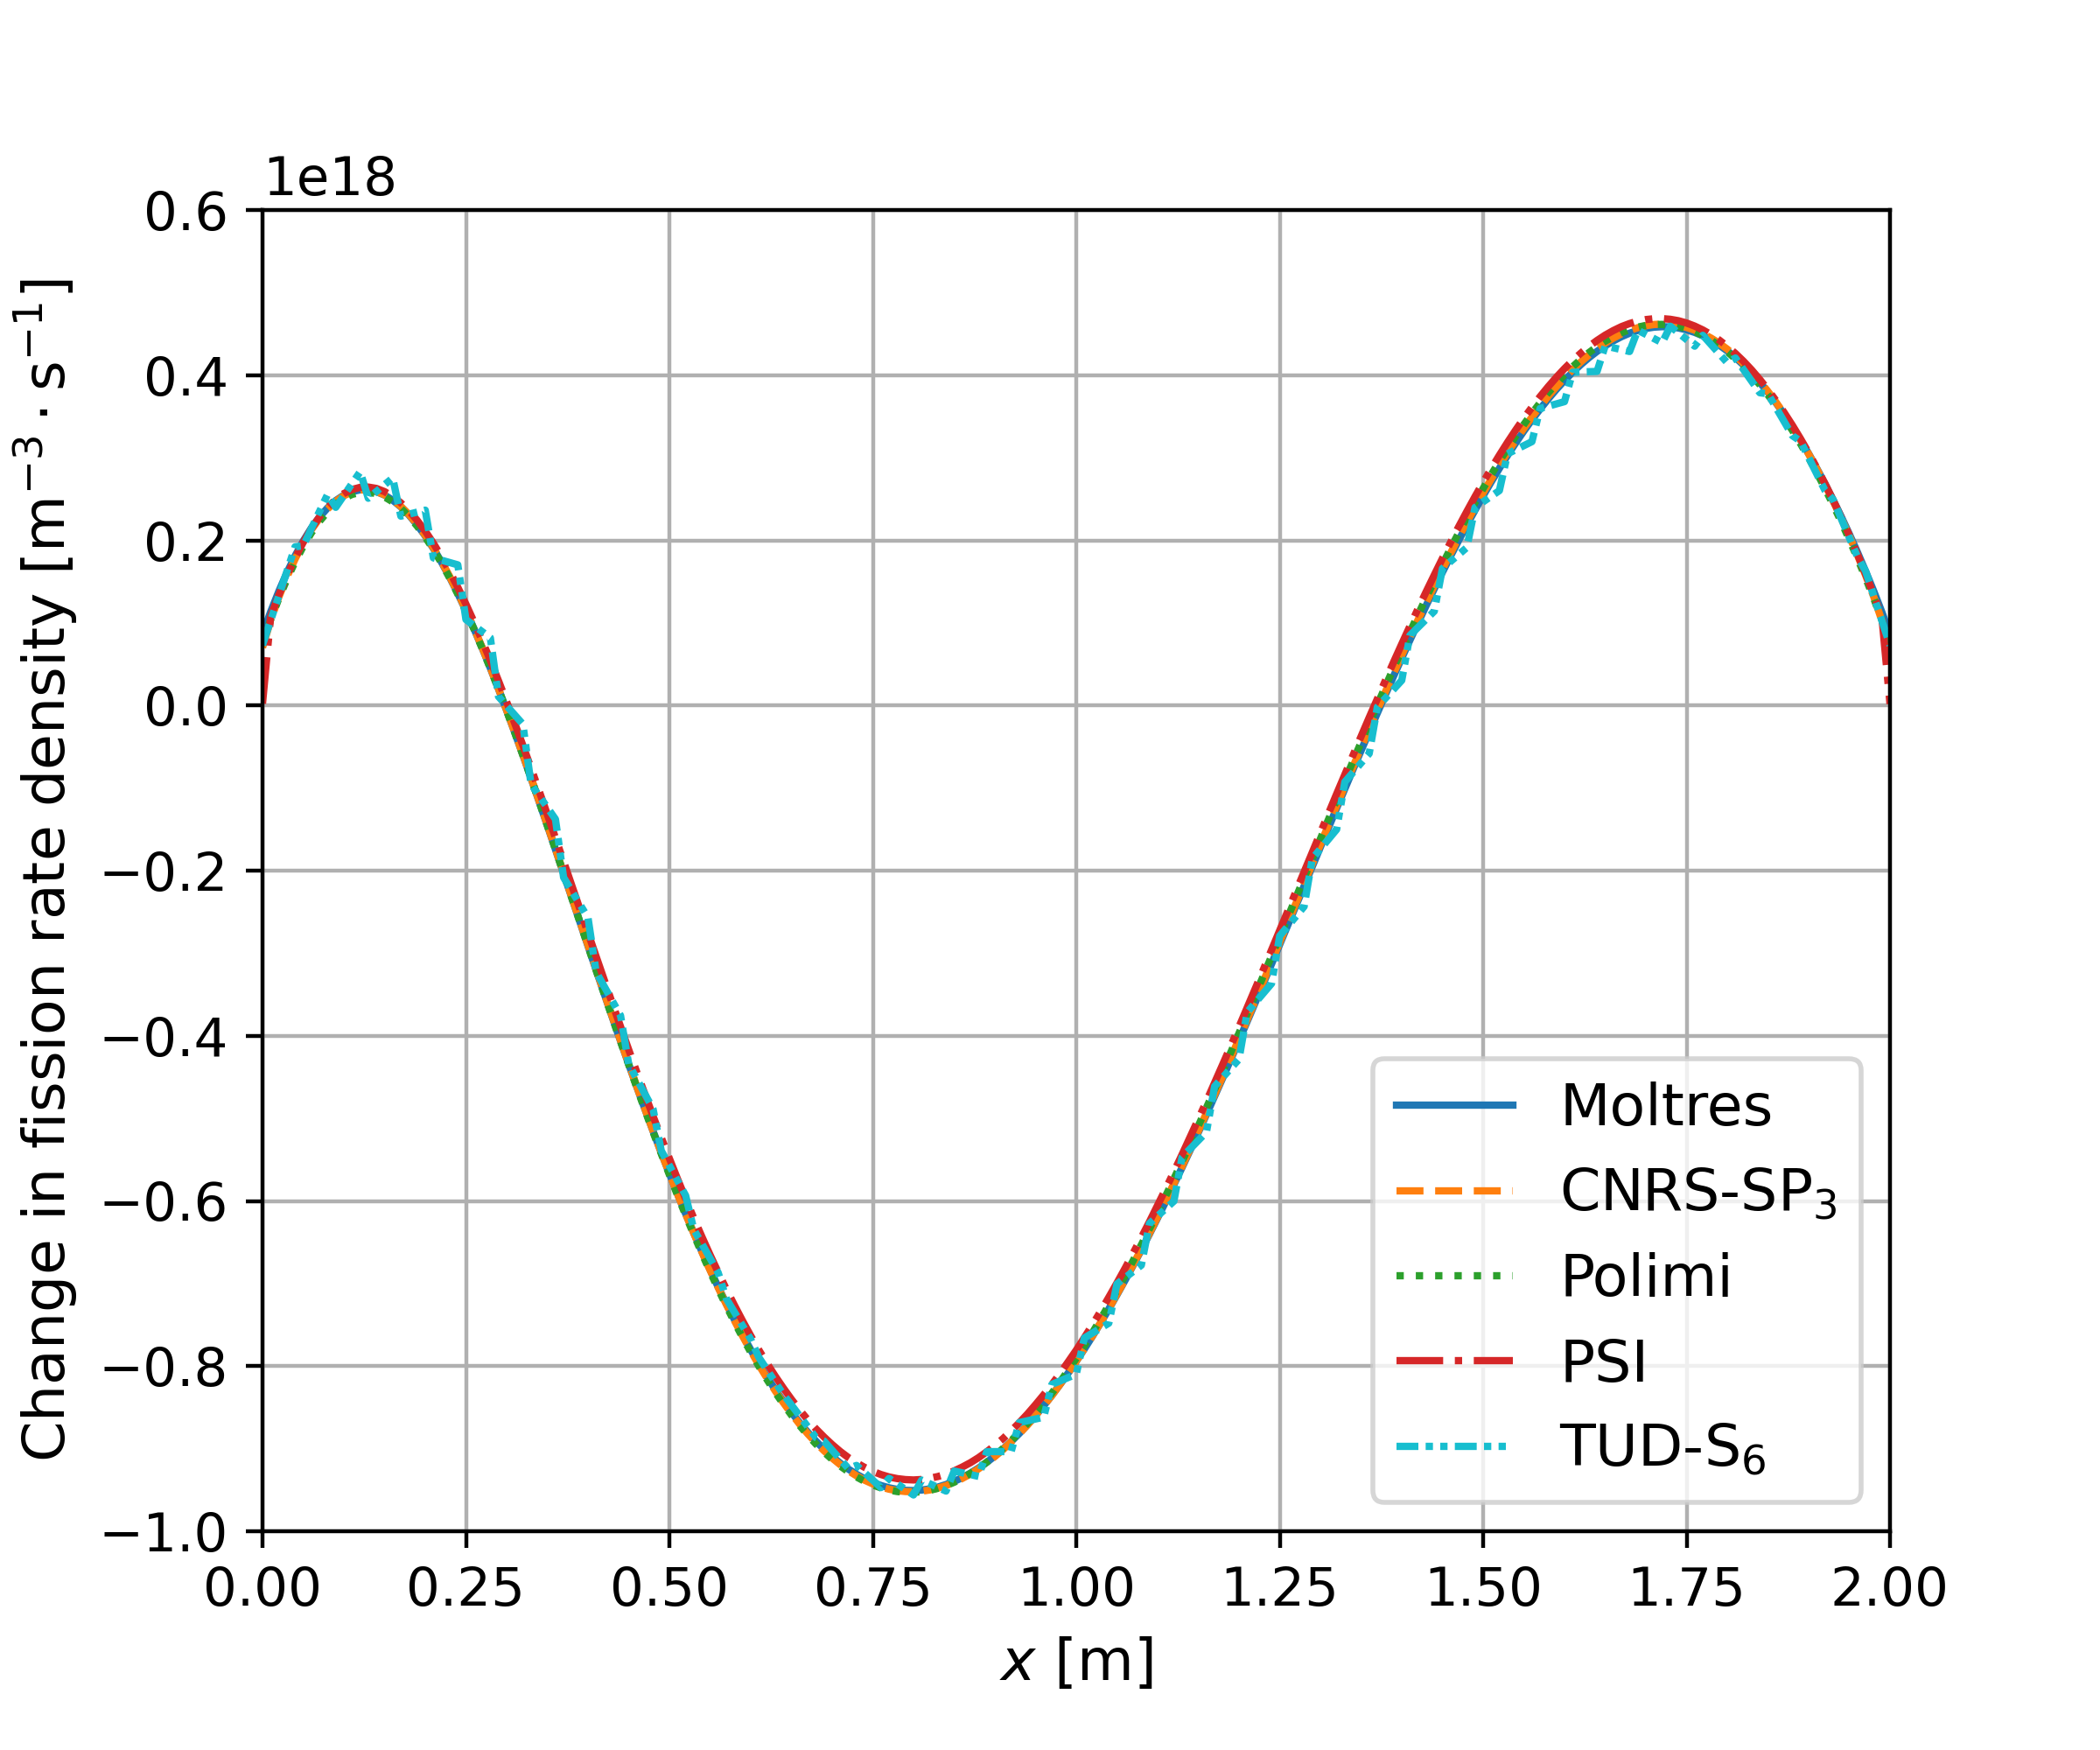
\includegraphics[width=.8\columnwidth]{1-2-fiss-plot}
	\caption{Step 1.2 \textemdash\ Temperature distribution and change in fission rate
	density along AA'.}
	\label{fig:1.2}
\end{figure*}

\FloatBarrier

\subsubsection{Step 1.2: Power coupling}

Figure \ref{fig:1.2} shows the temperature distribution and the change in
fission rate density along AA' from Step 1.2. Similar to Step 0.3, the
temperature distribution from Moltres agrees closest with CNRS-$SP_3$ and
TUD-$S_2$. Table \ref{table:disc1} reports the same trends we observed in Phase
0; the average discrepancy in temperature along BB' from Moltres for Step 1.2
is marginally higher than the benchmark while the average discrepancy in the
fission rate density is within one \gls{SD} range to the benchmark average.
From Table \ref{table:rho}, Moltres also reports a change in $\rho$
relative to Step 1.1 of $-1142.2$ pcm which
falls within the range of reported benchmark participants' values.

\subsubsection{Step 1.3: Buoyancy}

Figure \ref{fig:1.3} shows the vertical velocity component, temperature, and
delayed neutron source distributions along AA'.
Moltres reproduces the correct trend in all three physical
observables. Step 1.3 has a relatively slower buoyancy-driven flow profile with
no forced flow from the top boundary. Consequently, there are no temperature
deviations near the top boundary and we observe in Table \ref{table:disc1} that
the average discrepancy value of 0.070\% for the temperature distribution along
BB' is in much closer agreement to the benchmark value of 0.080\% compared to
the corresponding temperature discrepancy values for Step 0.3 and 1.2.

In Table \ref{table:rho}, we observe that the change in $\rho$ from
Moltres (-1207.7 pcm) falls within the range of reported benchmark values and
matches the software from TUD-$S_2$ (-1208.5 pcm) the closest. This is likely
by virtue of the similar solvers (diffusion and $S_2$ neutronics models) and
methods of solution (finite element method on uniform meshes) employed by our
respective software.
%
\begin{figure*}[htb]
	\centering
	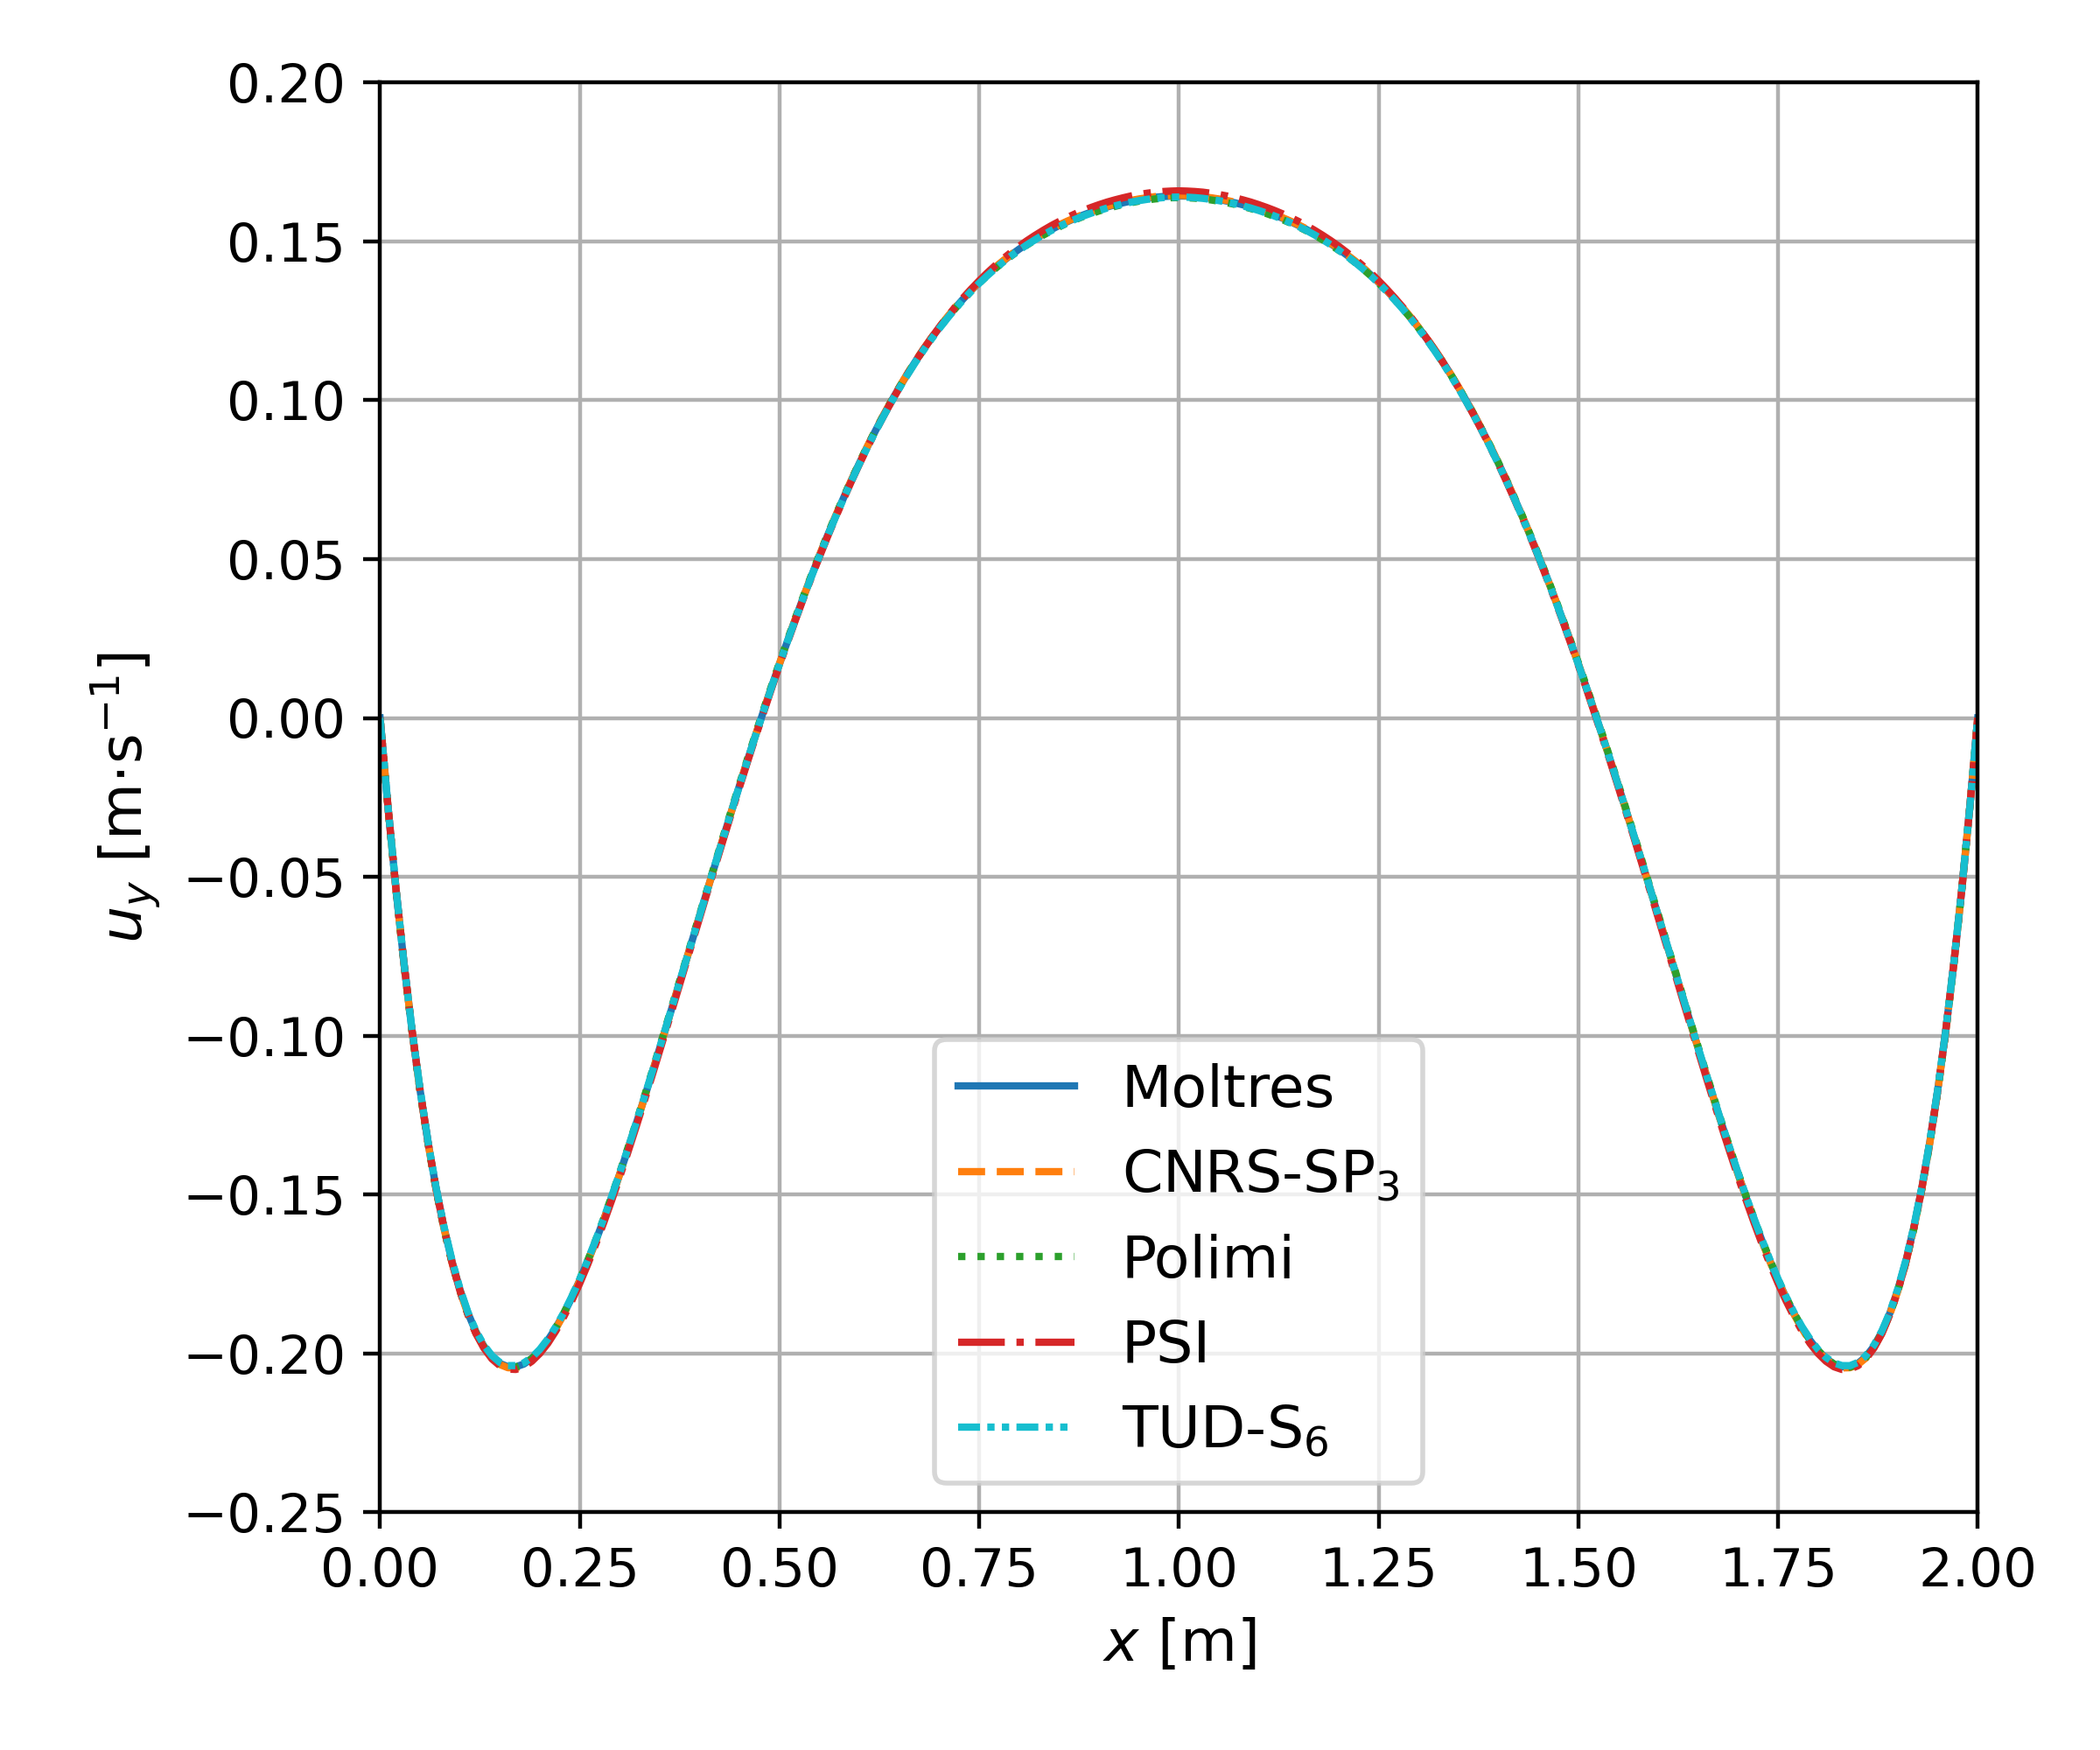
\includegraphics[width=.6\columnwidth]{1-3-vel-plot}
	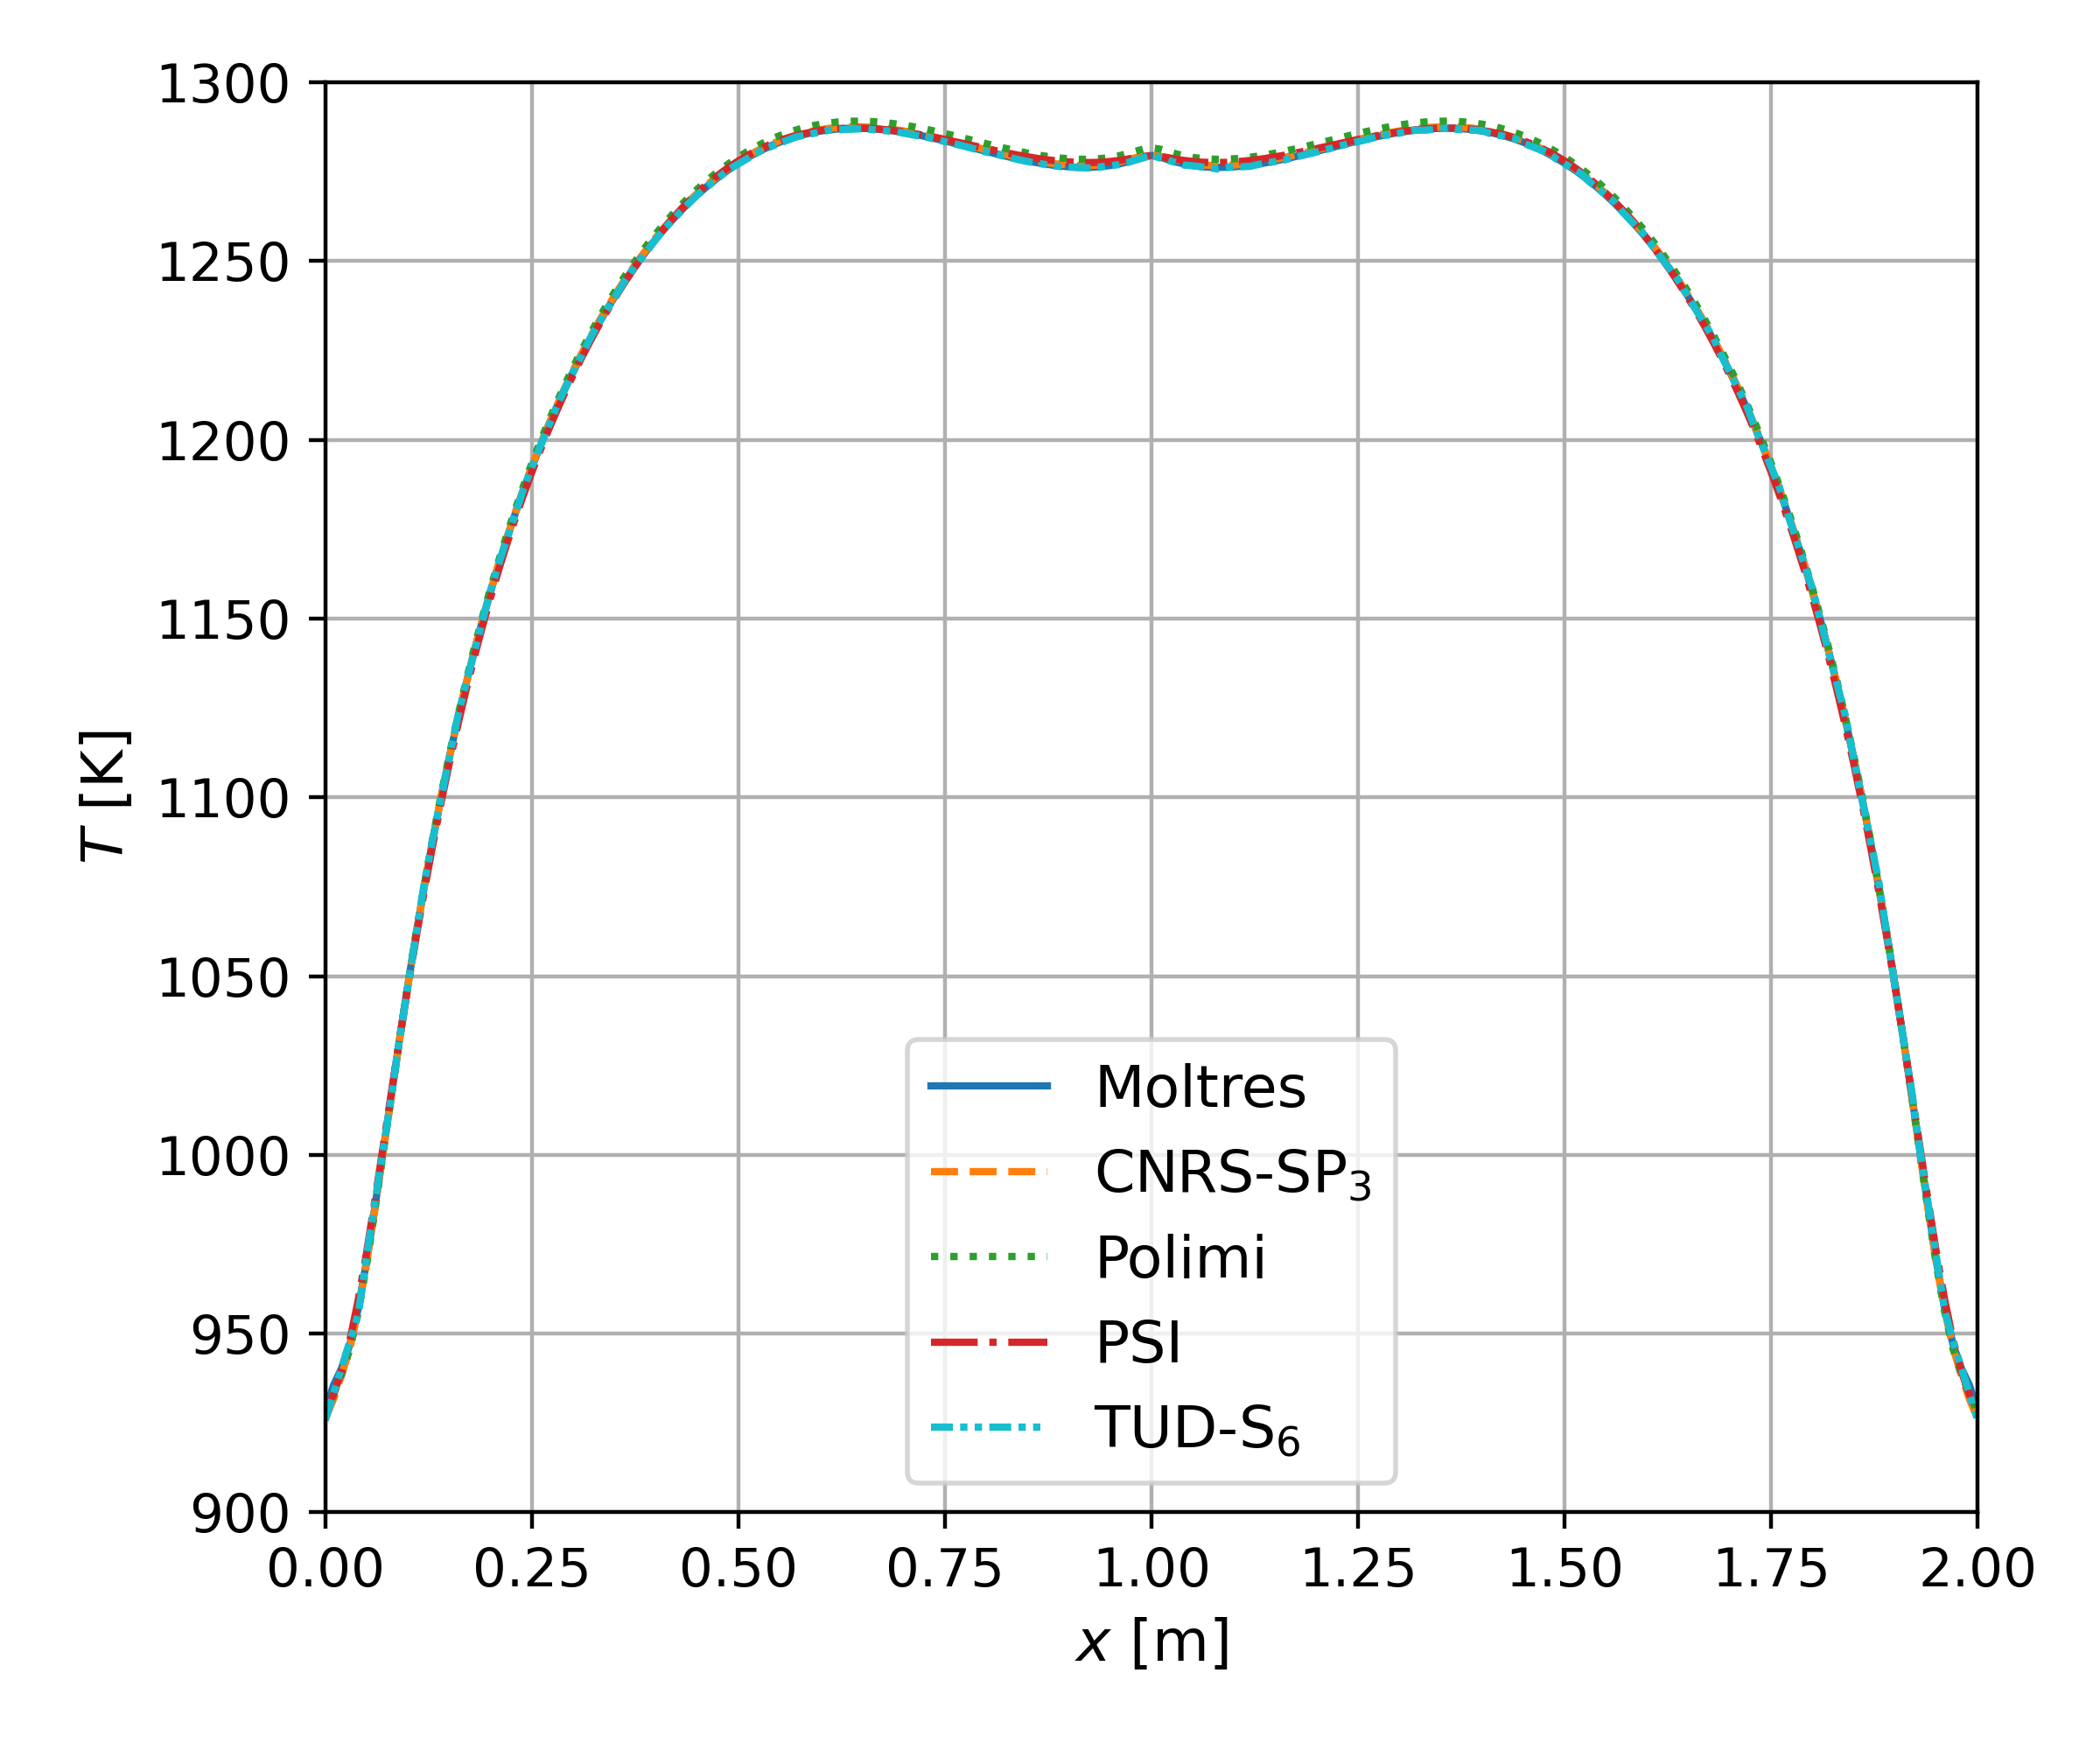
\includegraphics[width=.6\columnwidth]{1-3-temp-plot}
	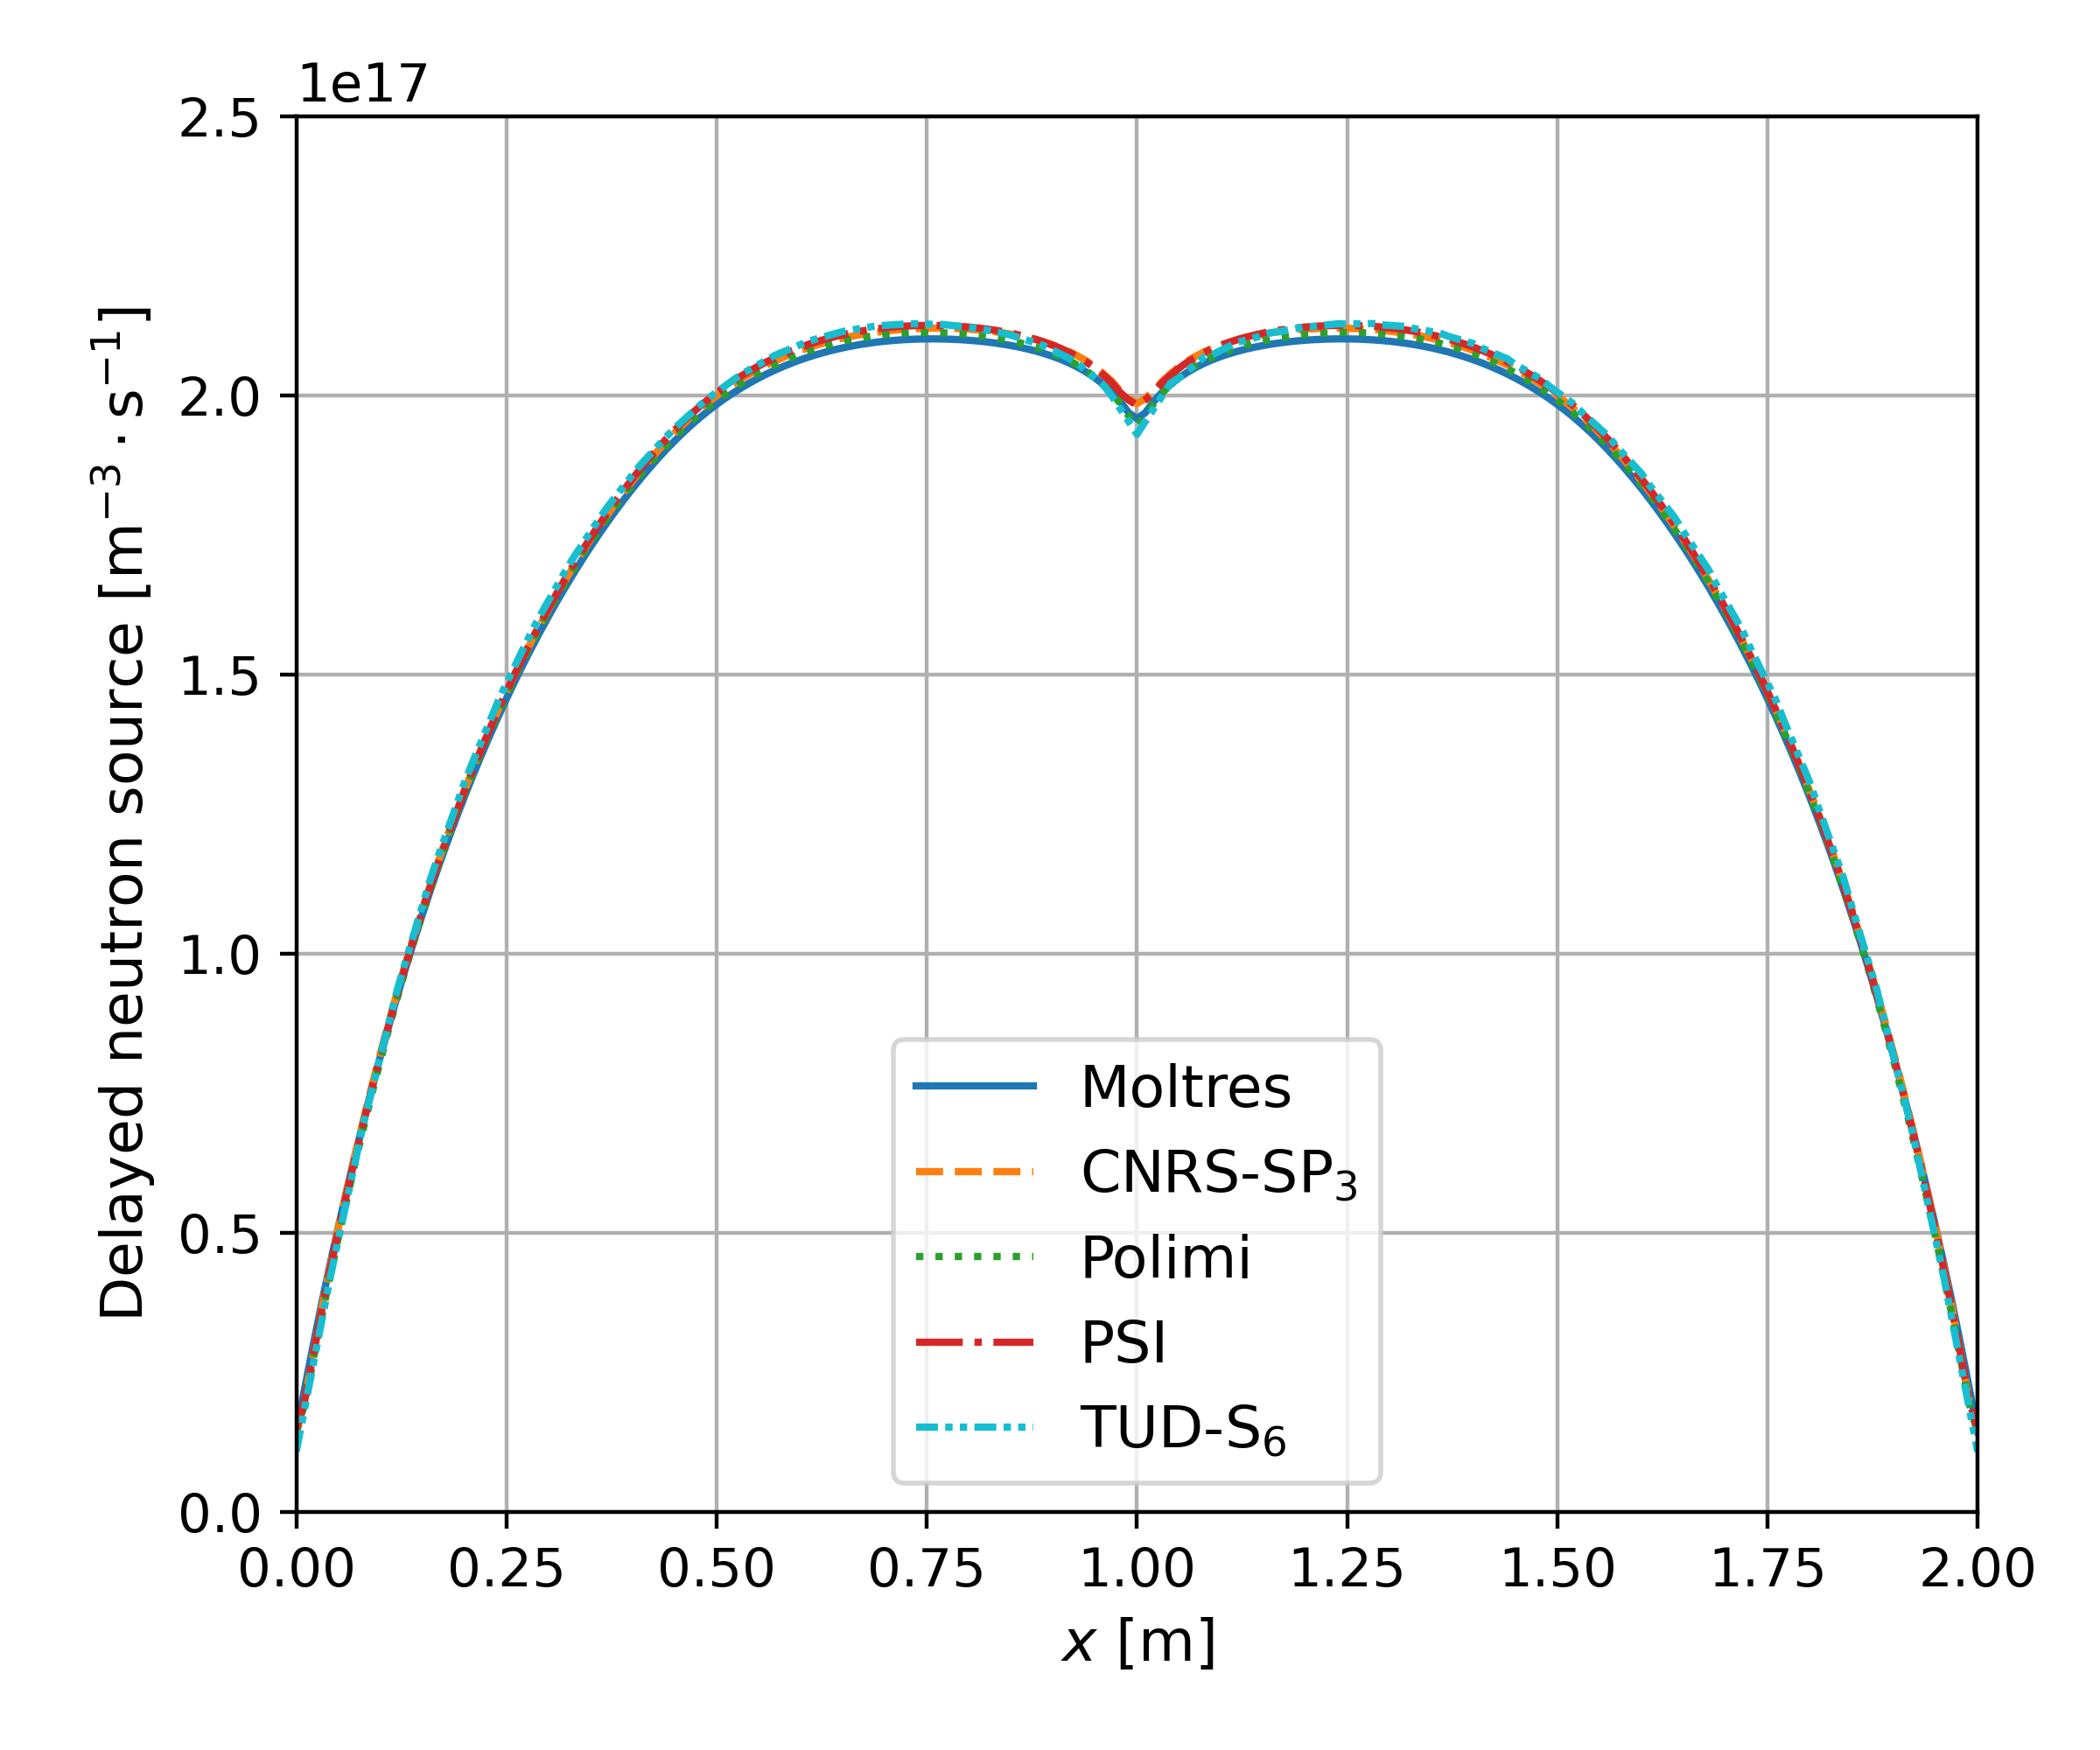
\includegraphics[width=.6\columnwidth]{1-3-dnp-plot}
	\caption{Step 1.3 \textemdash\ Vertical velocity component, temperature distribution,
	and delayed neutron source along AA'.}
	\label{fig:1.3}
\end{figure*}

\FloatBarrier

\subsubsection{Step 1.4: Full coupling}

Figure \ref{fig:color} shows 2D temperature distribution and velocity
streamlines from Moltres for Step 1.4 with $U_{lid} = 0.5$ m$\cdot$s$^{-1}$ and
$P = 1$ GW. Table \ref{table:full} shows the change in $\rho$ under the various
$U_{lid}$ and $P$ values. We refer readers to Tiberga et al.'s paper
\cite{tiberga_results_2020} for the benchmark participants' corresponding
values. The change in $\rho$ values from Moltres all fall within the range of
benchmark values
for all cases. Furthermore, the $\Delta\rho$ values are all within 1.1 pcm of
the corresponding values from the TUD-S$_2$ model in the benchmark paper. Given
that the $S_2$ discrete ordinates method is theoretically equivalent to the
multigroup neutron diffusion method, this indicates that Moltres is largely
consistent with the benchmark participants outside of differences from the
neutronics models.

\begin{figure}[htb]
  \centering
  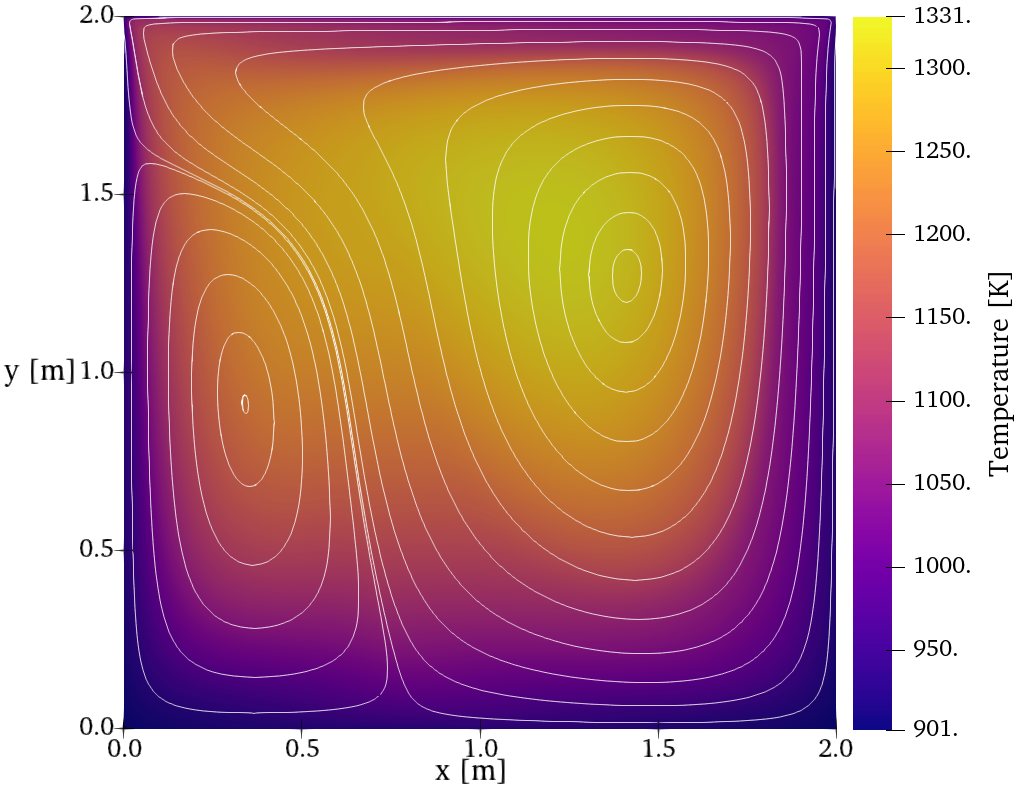
\includegraphics[width=\columnwidth]{full-coupled}
  \caption{Temperature distribution from Moltres for the fully coupled
  system (Step 1.4) with buoyancy effects, $P = 1$ GW, and $U_{lid} = 0.5$
  m$\cdot$s$^{-1}$. The lines correspond to the streamlines of the velocity
  field.}
  \label{fig:color}
\end{figure}
%
\begin{table}[htb]
	\caption{Reactivity change in Step 1.4, relative to Step 0.2 under various
	$U_{lid}$ and $P$ values.}
	\centering
	\small
	\setlength\tabcolsep{1.5pt}
	\begin{tabular}{c c c c c c}
		\toprule
		& \multicolumn{5}{c}{$\rho_{s1.4} - \rho_{s0.2}$ [pcm]} \\
		\midrule
		{\backslashbox{$U_{lid}$ [m$\cdot$s$^{-1}$]}{$P$ [GW]}} & 0.2 & 0.4 & 0.6 & 0.8 & 1.0 \\
		\midrule
		0.0 & -263.7 & -498.3 & -730.9 & -966.7 & -1207.7 \\
		0.1 & -265.9 & -498.7 & -730.6 & -966.0 & -1206.7 \\
		0.2 & -268.1 & -498.8 & -729.4 & -963.7 & -1203.6 \\
		0.3 & -269.9 & -498.5 & -727.8 & -960.8 & -1199.5 \\
		0.4 & -271.9 & -498.5 & -726.5 & -958.3 & -1195.7 \\
		0.5 & -274.2 & -498.7 & -725.6 & -956.4 & -1192.7 \\
		\bottomrule
	\end{tabular}
	\label{table:full}
\end{table}

\FloatBarrier

\begin{table}[htb]
	\caption{Discrepancy values from Moltres alongside the average and standard
	deviation of the discrepancy values of the benchmark participants for Step
	2.1.}
	\centering
	\small
	\begin{tabular}{l l S S S}
		\toprule
		\multirow{2}{*}{\textbf{Step}} & \multirow{2}{*}{\textbf{Observable}} & {\multirow{2}{*}{\textbf{Moltres [\%]}}} & \multicolumn{2}{c}{\textbf{Benchmark [\%]}} \\
		& & & {Average} & {SD} \\
		\midrule
		\multirow{2}{*}{2.1} & Gain & 0.493 & 0.587 & 0.244 \\
		\cmidrule{2-5}
		& Phase shift & 1.741 & 2.176 & 0.554 \\
		\bottomrule
	\end{tabular}
	\label{table:disc2}
\end{table}
%
\begin{figure*}[htb]
	\centering
	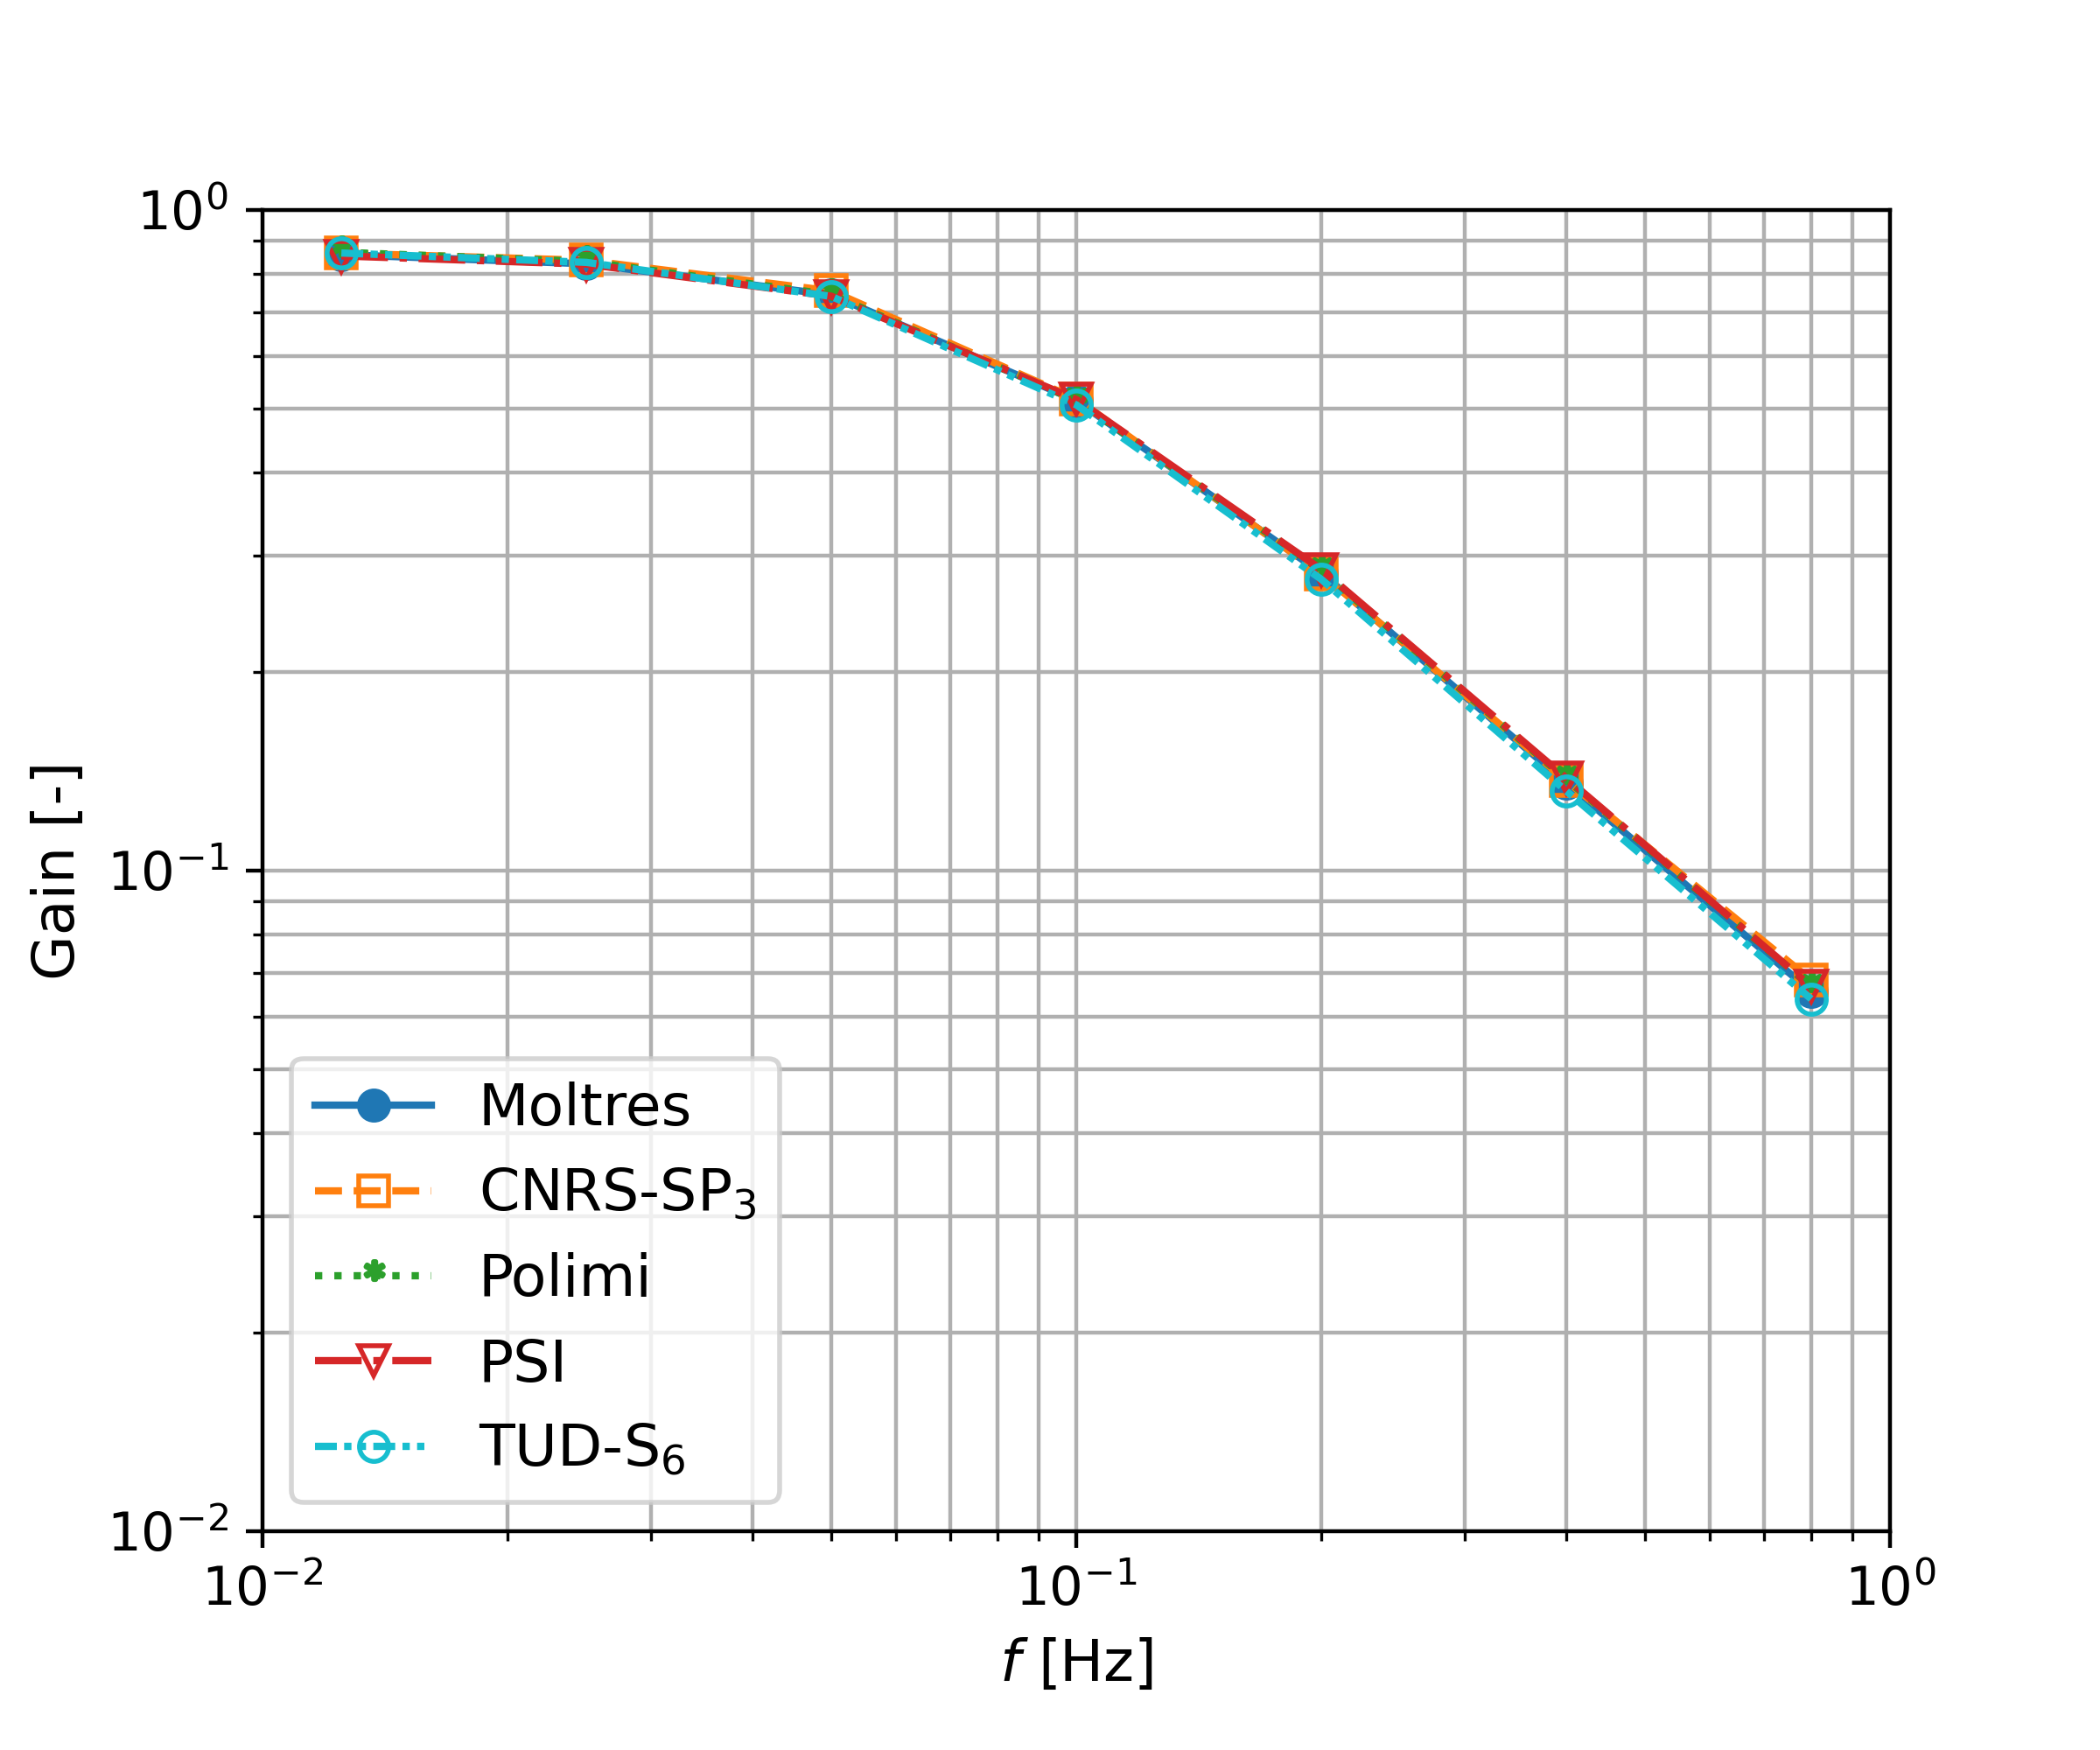
\includegraphics[width=.8\columnwidth]{2-1-gain-plot}
	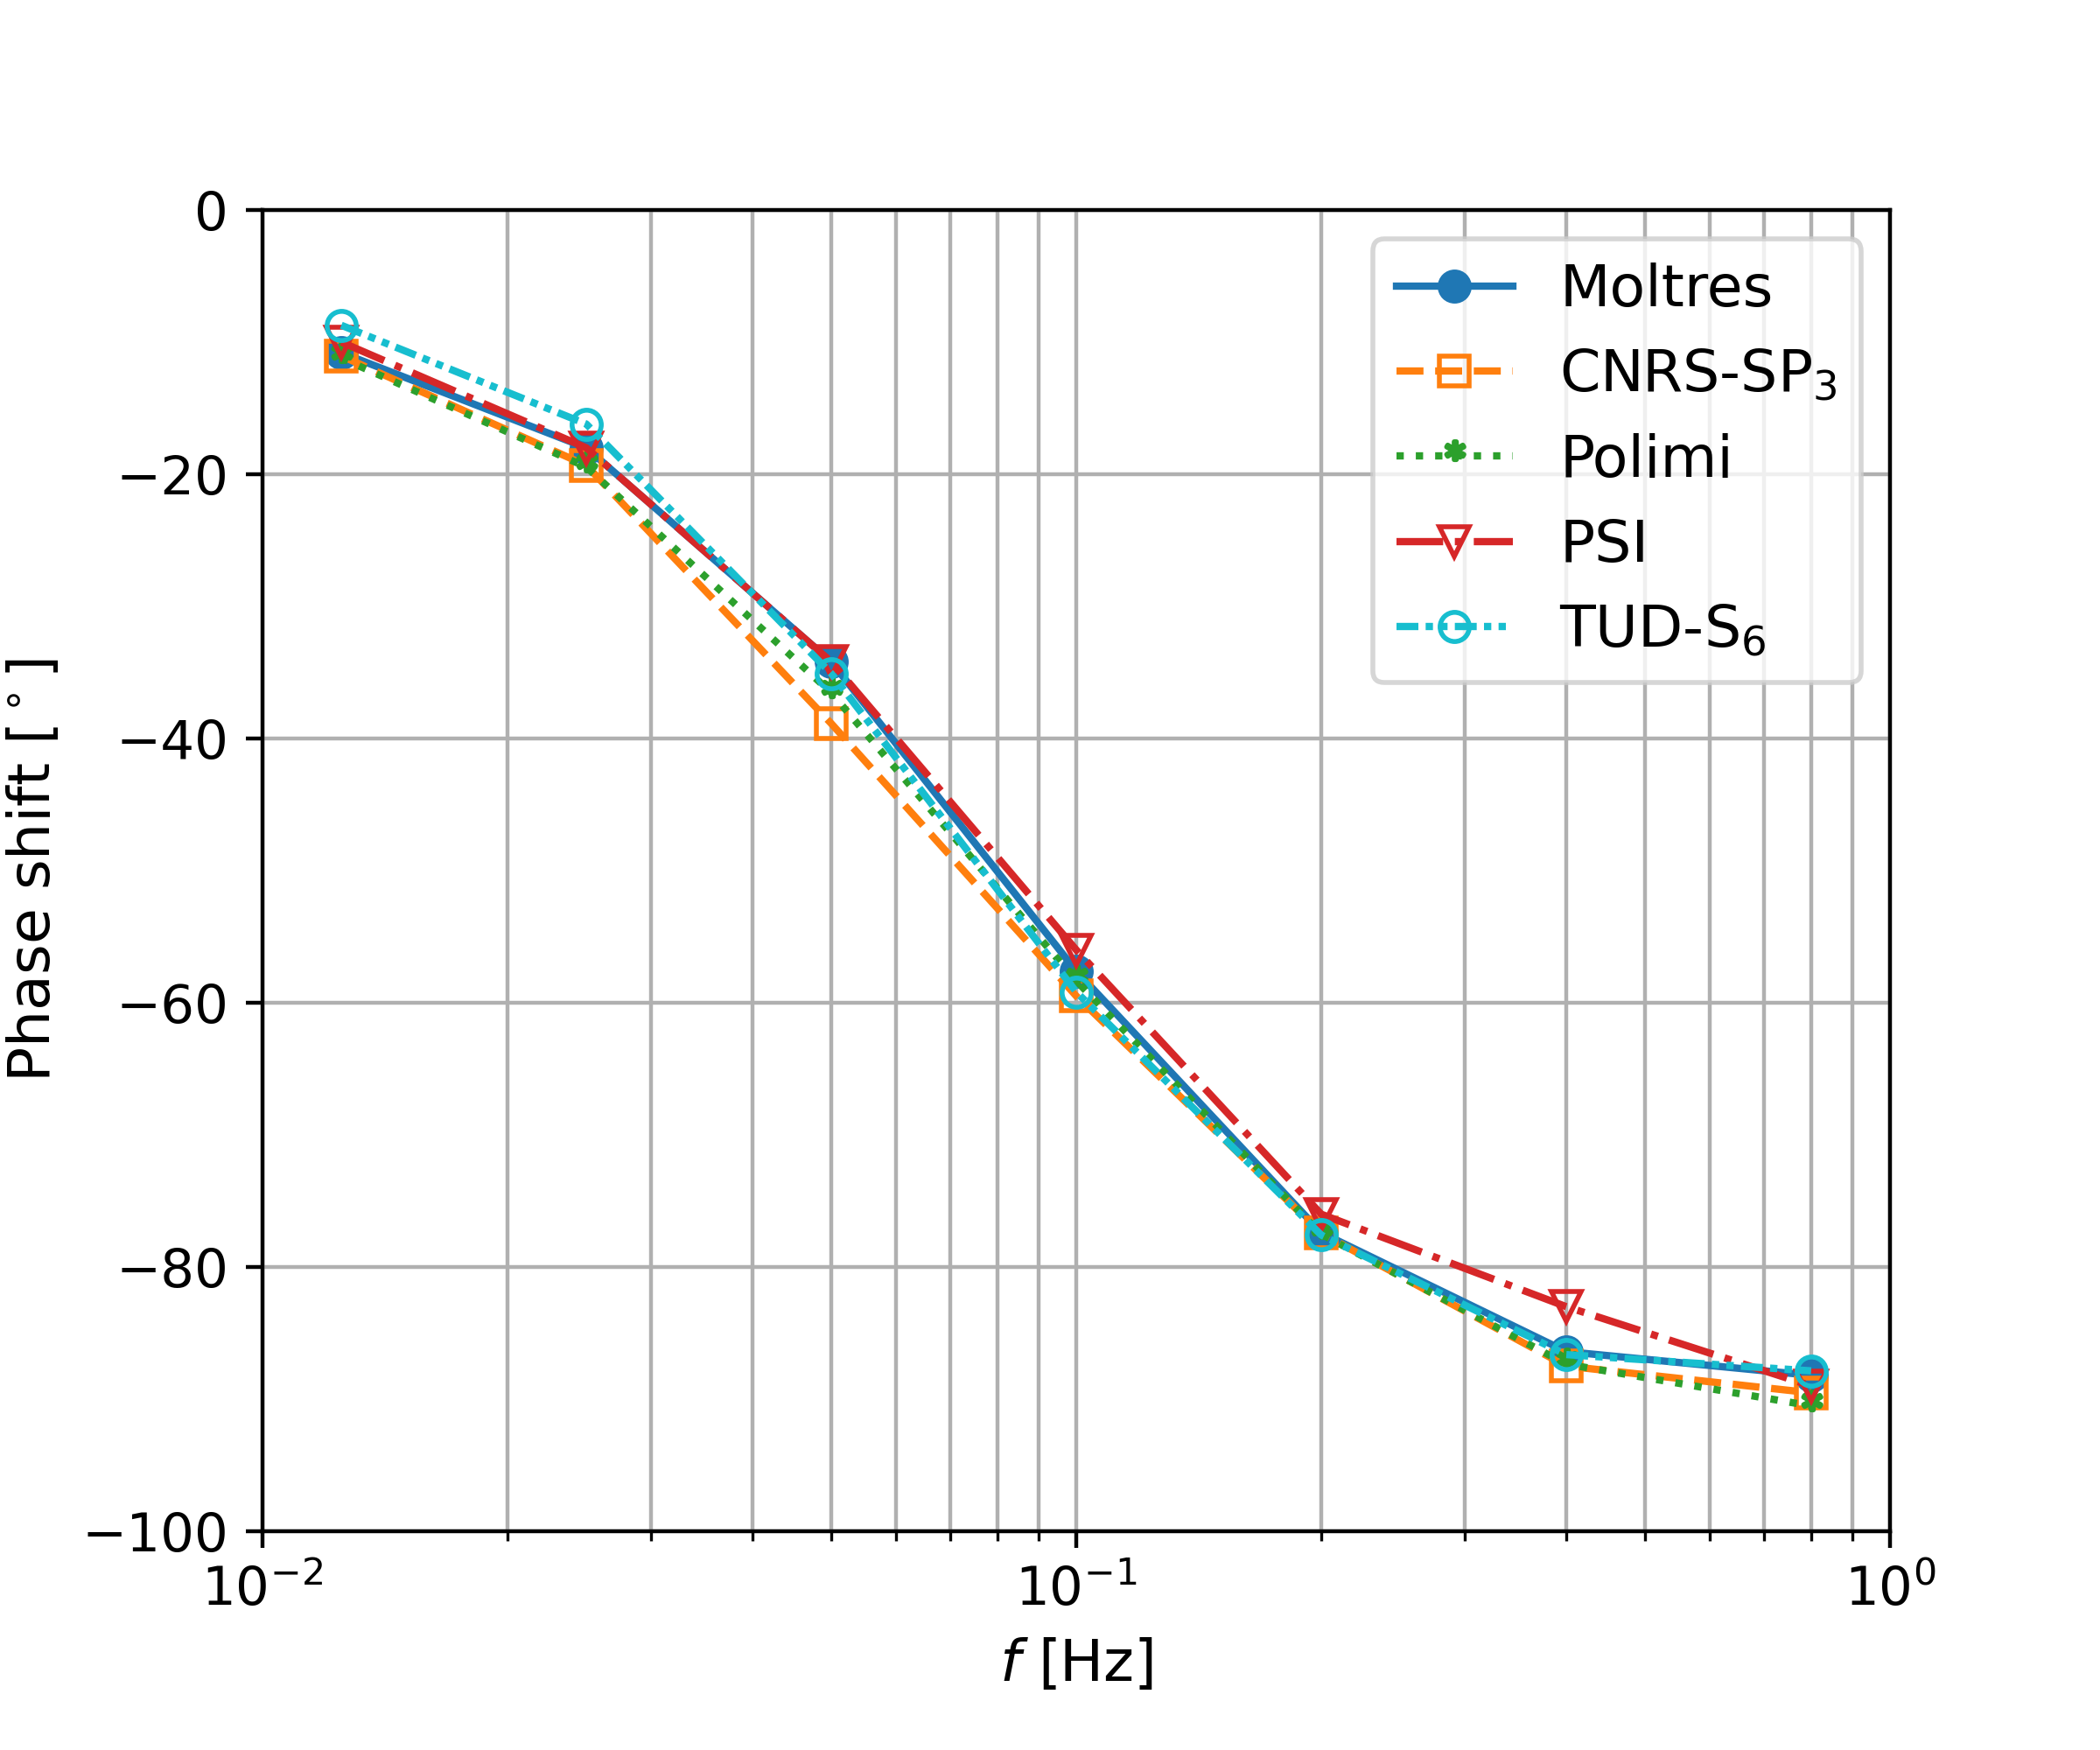
\includegraphics[width=.8\columnwidth]{2-1-phase-plot}
	\caption{Step 2.1 \textemdash\ Bode gain and phase plots of the frequency response of
	the fully coupled system.}
	\label{fig:2.1}
\end{figure*}

\subsection{Phase 2 results \& discussion}

Lastly, the following subsection discusses the results for the transient cases
in Step 2.1 which involve measuring the response in power output to periodic
perturbations in the heat transfer coefficient.

\subsubsection{Step 2.1: Forced convection transient}

Figure \ref{fig:2.1} shows the Bode gain and phase shift plots of the response
in power output in the fully coupled system. Along with the average discrepancy
values from Table \ref{table:disc2}, the results show that Moltres is
consistent with the benchmark. The gain data points from all \gls{MSR} software
agree closely with one another. Moltres reports an average discrepancy value of
0.496\%, slightly lower than the benchmark average of 0.587\%. On the other
hand, the phase shift data points show greater spread over the various driving
frequencies. We note the different timestepping schemes and timestep
sizes among the different software packages which is likely responsible for
the variations in the phase shift. Even with a precision of
$\pm0.9^\circ$ for each phase shift value, Moltres accurately reproduces the
correct trend with a lower average discrepancy (1.741\%) than the benchmark
participants' average (2.176\%).

\subsection{Computational performance}

We ran all of the simulations on Cray XE nodes on the Blue Waters
supercomputer. Each XE node is comprised of two AMD Opteron\texttrademark\ 6276
processors, for a total of 32 CPU cores per node, rated at a maximum clock
speed of 3.2 GHz. Lindsay et al. \cite{lindsay_introduction_2018} previously
reported good scaling performance of Moltres on the Blue Waters system.

While the simulations for Phases 0 and 1 were not computationally intensive,
some required more memory than the 8GB to 16GB typically available on most
personal computers. Table \ref{table:compute} shows the compute times required
per perturbation cycle of the highest and lowest perturbation frequencies for
Step 2.1 on 16 XE nodes. The compute times of all other simulations in Step 2.1
fall between 0.98h and 6.29h. The simulations with smaller perturbation
frequencies required longer compute times because the larger timestep sizes led
to greater changes in the variables per timestep. The compute times are
comparable to the compute times for the CNRS-$SP_1$ and CNRS-$SP_3$ models on
20 Intel\textsuperscript{\tiny\textregistered}
Xeon\textsuperscript{\tiny\textregistered} Gold 5118 processors reported in
\cite{blanco_neutronic_2021,blanco_neutronic_2020}.

\begin{table}[htb]
	\caption{Compute times required for one perturbation cycle in Step 2.1 for
	$f=0.0125$ Hz and $0.8$ Hz on 16 XE nodes (512 CPU cores).}
	\centering
	\small
	\setlength\tabcolsep{1.5pt}
	\begin{tabular}{l S S}
		\toprule
		$f$ [Hz] & 0.0125 & 0.8 \\
		\midrule
		Compute time [hours] & 6.29 & 0.98 \\
		\bottomrule
	\end{tabular}
	\label{table:compute}
\end{table}

\FloatBarrier

\section{Conclusions}

\glspl{MSR} feature significant multiphysics interactions which present
computational challenges for many existing multiphysics reactor analysis
software. This paper presents code-to-code verification of Moltres
capabilities in modeling such multiphysics phenomena in fast-spectrum
\glspl{MSR} based on the CNRS benchmark \cite{tiberga_results_2020}.
The CNRS benchmark assesses multiphysics \gls{MSR} simulation
software through several steps involving single-physics and coupled
neutronics/thermal-hydraulics problems.

The results showed that Moltres is consistent with the participating software
presented in the CNRS benchmark paper for the modeling of important phenomena
in fast-spectrum \glspl{MSR}. The percentage discrepancies in the various
neutronics, velocity, and temperature quantities mostly fall below or within
one standard deviation of the average of the benchmark participants.
Minor deviations in the temperature in Steps 0.3 and 1.2 
stem from the discontinuous velocity
boundaries on the top corners in the lid-driven cavity flow. We have shown that
these deviations are limited to the top boundary of the domain and do not
affect the rest of the physical parameters. The results from
Moltres agree closest with the TUD-S$_2$ software package, which implements the
$S_2$ discrete ordinates method for
neutron transport on a uniform structured mesh with a \gls{DGFEM}-based solver.
These features make Moltres the most similar to the TUD-$S_2$ model as compared
to the other models which employ different neutron transport models,
non-uniform meshes, and/or finite volume-based solvers.

This work verifies Moltres' capabilities for future work involving modeling and
simulation of fast-spectrum \glspl{MSR}. Fast-spectrum \glspl{MSR}
under consideration for modeling with Moltres include the European \gls{MSFR}
as a continuation of work done in \cite{park_advancement_2020}, and
TerraPower's \gls{MCFR} \cite{terrapower_terrapower_2021} from publicly
available design specifications. Moltres can play an important role in
supporting further \gls{MSR} development through enabling transient accident
safety analysis and design optimization studies on an open-source platform.
An ongoing research project involves employing Moltres as a
surrogate model for machine learning-based reactor design optimization.
We note that Moltres also supports modeling solid-fueled reactors such as the
\gls{HTGR} by disabling the precursor drift functionality as demonstrated by
\cite{fairhurst-agosta_multi-physics_2020}. Future work pertaining to
further Moltres development include introducing an intermediate-fidelity
turbulence model for highly turbulent flows in \glspl{MSR}, improving
neutronics accuracy in heterogenous geometries, and enhancing the general
computational performance of existing features.

\FloatBarrier

\section{Acknowledgments}
This research is part of the Blue Waters sustained-petascale computing project,
which is supported by the National Science Foundation (awards OCI-0725070 and
ACI-1238993) and the state of Illinois. Blue Waters is a joint effort of the
University of Illinois at Urbana-Champaign and its National Center for
Supercomputing Applications.

Sun Myung Park is supported by the SNRSI Postgraduate Scholarship program, a
graduate fellowship program from the Singapore Nuclear Research \& Safety
Initiative.


\bibliography{bibliography}

% Prof. Huff discourages appendices in journal articles.
% But, if you must, include one like so:
\pagebreak
\appendix
\section{Additional data tables} \label{appendix:tables}

This Appendix presents observable values measured at nine
equidistant points along the centerlines AA' and BB' from Moltres and the
CNRS benchmark participants \cite{tiberga_results_2020}. We refer readers to
\cite{park_results_2021} and \cite{tiberga_results_2019} for the full set of
results from Moltres and the benchmark participants. 

\begin{table}[htbp!]
	\caption{Step 0.1 - Velocity components along centerlines AA' and BB'.}
	\centering
	\footnotesize
	\setlength\tabcolsep{1.5pt}
	\hspace*{-2cm}
	\renewcommand{\arraystretch}{.8}
	\begin{tabular}{c c c c c c c c c c c}
		\toprule
		\multirow{2}{*}{\textbf{Observable}} & \multirow{2}{*}{\textbf{Code}} & \multicolumn{9}{c}{\textbf{Results along $AA'$} (point coordinates are expressed in m)} \\
		& & {(0,1)} & {(0.25,1)} & {(0.5,1)} & {(0.75,1)} & {(1,1)} & {(1.25,1)} & {(1.5,1)} & {(1.75,1)} & {(2,1)} \\
		\midrule
		\multirow{5}{*}{$u_x$ (m s$^{-1}$)} & Moltres & 0.000E+00 & -1.923E-02 & -5.372E-02 & -8.371E-02 & -1.025E-01 & -1.043E-01 & -7.975E-02 & -3.080E-02 & 0.000E+00 \\
		& CNRS & 0.000E+00 & -1.924E-02 & -5.372E-02 & -8.369E-02 & -1.025E-01 & -1.043E-01 & -7.972E-02 & -3.080E-02 & 0.000E+00 \\
        & PoliMi & 0.000E+00 & -1.922E-02 & -5.365E-02 & -8.357E-02 & -1.023E-01 & -1.041E-01 & -7.947E-02 & -3.066E-02 & 0.000E+00 \\
        & PSI & 0.000E+00 & -1.929E-02 & -5.366E-02 & -8.332E-02 & -1.018E-01 & -1.034E-01 & -7.912E-02 & -3.072E-02 & 0.000E+00 \\
        & TUD & 1.002E-06 & -1.922E-02 & -5.372E-02 & -8.371E-02 & -1.025E-01 & -1.044E-01 & -7.977E-02 & -3.081E-02 & 4.198E-06 \\
        \midrule
		\multirow{5}{*}{$u_y$ (m s$^{-1}$)} & Moltres & 0.000E+00 & 7.269E-02 & 8.579E-02 & 6.087E-02 & 1.250E-02 & -4.794E-02 & -9.612E-02 & -8.722E-02 & 0.000E+00\\
		& CNRS & 0.000E+00 & 7.266E-02 & 8.575E-02 & 6.084E-02 & 1.251E-02 & -4.789E-02 & -9.606E-02 & -8.722E-02 & 0.000E+00 \\
        & PoliMi & 0.000E+00 & 7.139E-02 & 8.433E-02 & 6.007E-02 & 1.269E-02 & -4.691E-02 & -9.472E-02 & -8.621E-02 & 0.000E+00 \\
        & PSI & 0.000E+00 & 7.265E-02 & 8.534E-02 & 6.021E-02 & 1.230E-02 & -4.734E-02 & -9.536E-02 & -8.720E-02 & 0.000E+00 \\
        & TUD & 5.877E-06 & 7.269E-02 & 8.580E-02 & 6.089E-02 & 1.252E-02 & -4.794E-02 & -9.613E-02 & -8.726E-02 & -1.013E-05 \\
		\midrule
		\midrule
		\multirow{2}{*}{\textbf{Observable}} & \multirow{2}{*}{\textbf{Code}} & \multicolumn{9}{c}{\textbf{Results along $BB'$} (point coordinates are expressed in m)} \\
		& & {(1,0)} & {(1,0.25)} & {(1,0.5)} & {(1,0.75)} & {(1,1)} & {(1,1.25)} & {(1,1.5)} & {(1,1.75)} & {(1,2)} \\
		\midrule
		\multirow{5}{*}{$u_x$ (m s$^{-1}$)} & Moltres & 0.000E+00 & -3.518E-02 & -6.243E-02 & -8.723E-02 & -1.025E-01 & -8.770E-02 & -1.146E-02 & 1.718E-01 & 5.000E-01 \\
		& CNRS & 0.000E+00 & -3.517E-02 & -6.242E-02 & -8.720E-02 & -1.025E-01 & -8.766E-02 & -1.147E-02 & 1.717E-01 & 5.000E-01 \\
        & PoliMi & 0.000E+00 & -3.423E-02 & -6.107E-02 & -8.613E-02 & -1.023E-01 & -8.861E-02 & -1.299E-02 & 1.706E-01 & 5.000E-01 \\
        & PSI & 0.000E+00 & -3.511E-02 & -6.217E-02 & -8.667E-02 & -1.018E-01 & -8.731E-02 & -1.191E-02 & 1.705E-01 & 5.000E-01 \\
        & TUD & 1.494E-06 & -3.519E-02 & -6.244E-02 & -8.724E-02 & -1.025E-01 & -8.770E-02 & -1.146E-02 & 1.718E-01 & 5.000E-01 \\
        \midrule
		\multirow{5}{*}{$u_y$ (m s$^{-1}$)} & Moltres & 0.000E+00 & 5.161E-05 & 6.166E-04 & 3.842E-03 & 1.250E-02 & 2.525E-02 & 3.050E-02 & 1.501E-02 & 0.000E+00 \\
		& CNRS & 0.000E+00 & 5.641E-05 & 6.309E-04 & 3.862E-03 & 1.251E-02 & 2.524E-02 & 3.048E-02 & 1.500E-02 & 0.000E+00 \\
        & PoliMi & 0.000E+00 & 9.118E-05 & 7.484E-04 & 4.046E-03 & 1.269E-02 & 2.534E-02 & 3.050E-02 & 1.500E-02 & 0.000E+00 \\
        & PSI & 0.000E+00 & 7.727E-05 & 6.822E-04 & 3.875E-03 & 1.230E-02 & 2.472E-02 & 2.994E-02 & 1.481E-02 & 0.000E+00 \\
        & TUD & 1.501E-06 & 5.260E-05 & 6.209E-04 & 3.853E-03 & 1.252E-02 & 2.528E-02 & 3.053E-02 & 1.502E-02 & 7.987E-06 \\
		\bottomrule
	\end{tabular}
\end{table}

\begin{table}[htbp!]
	\caption{Step 0.2 - Fission rate density along $AA'$.}
	\centering
	\footnotesize
	\setlength\tabcolsep{1.5pt}
	\hspace*{-2cm}
	\renewcommand{\arraystretch}{.8}
	\begin{tabular}{c c c c c c c c c c c}
		\toprule
		\multirow{2}{*}{\textbf{Observable}} & \multirow{2}{*}{\textbf{Code}} & \multicolumn{9}{c}{\textbf{Results along $AA'$} (point coordinates are expressed in m)} \\
		& & {(0,1)} & {(0.25,1)} & {(0.5,1)} & {(0.75,1)} & {(1,1)} & {(1.25,1)} & {(1.5,1)} & {(1.75,1)} & {(2,1)} \\
		\midrule
		\multirow{7}{*}{\shortstack[1]{$\int_E \Sigma_f \Phi$d$E$\\(m$^{-3}$s$^{-1}$)}} & Moltres & 7.701E+17 & 7.461E+18
		& 1.303E+19 & 1.672E+19 & 1.801E+19 & 1.672E+19 & 1.303E+19 &
		7.461E+18 & 7.701E+17 \\
		& CNRS-$SP_1$ & 6.896E+17 & 7.436E+18 & 1.305E+19 & 1.678E+19 & 1.809E+19 & 1.678E+19 & 1.305E+19 & 7.436E+18 & 6.896E+17 \\
		& CNRS-$SP_3$ & 6.206E+17 & 7.450E+18 & 1.303E+19 & 1.673E+19 & 1.802E+19 & 1.673E+19 & 1.303E+19 & 7.450E+18 & 6.206E+17 \\
		& PoliMi & 7.780E+17 & 7.470E+18 & 1.310E+19 & 1.684E+19 & 1.815E+19 & 1.684E+19 & 1.310E+19 & 7.470E+18 & 7.780E+17 \\
		& PSI & 8.622E+17 & 7.436E+18 & 1.305E+19 & 1.678E+19 & 1.809E+19 & 1.678E+19 & 1.305E+19 & 7.436E+18 & 8.622E+17 \\
		& TUD-$S_2$ & 6.626E+17 & 7.433E+18 & 1.307E+19 & 1.682E+19 & 1.814E+19 & 1.682E+19 & 1.307E+19 & 7.433E+18 & 6.626E+17 \\
		& TUD-$S_6$ & 6.833E+17 & 7.463E+18 & 1.300E+19 & 1.667E+19 & 1.796E+19 & 1.667E+19 & 1.300E+19 & 7.463E+18 & 6.833E+17 \\
		\bottomrule
	\end{tabular}
\end{table}

\begin{table}[htbp!]
	\caption{Step 0.3 - Temperature distribution along centerlines $AA'$ and $BB'$.}
	\label{table:0.3}
	\centering
	\footnotesize
	\setlength\tabcolsep{1.5pt}
	\hspace*{-2cm}
	\renewcommand{\arraystretch}{.8}
	\begin{tabular}{c c c c c c c c c c c}
		\toprule
		\multirow{2}{*}{\textbf{Observable}} & \multirow{2}{*}{\textbf{Code}} & \multicolumn{9}{c}{\textbf{Results along $AA'$} (point coordinates are expressed in m)} \\
		& & {(0,1)} & {(0.25,1)} & {(0.5,1)} & {(0.75,1)} & {(1,1)} & {(1.25,1)} & {(1.5,1)} & {(1.75,1)} & {(2,1)} \\
		\midrule
		\multirow{7}{*}{$T$ (K)} & Moltres & 9.251E+02 & 1.194E+03 & 1.357E+03 & 1.361E+03 &
		1.303E+03 & 1.224E+03 & 1.131E+03 & 1.035E+03 & 9.251E+02 \\
		& CNRS-$SP_1$ & 9.253E+02 & 1.194E+03 & 1.358E+03 & 1.363E+03 & 1.305E+03 & 1.224E+03 & 1.131E+03 & 1.034E+03 & 9.251E+02 \\
		& CNRS-$SP_3$ & 9.236E+02 & 1.194E+03 & 1.357E+03 & 1.361E+03 & 1.304E+03 & 1.224E+03 & 1.131E+03 & 1.034E+03 & 9.235E+02 \\
		& PoliMi & 9.253E+02 & 1.196E+03 & 1.361E+03 & 1.364E+03 & 1.305E+03 & 1.224E+03 & 1.132E+03 & 1.035E+03 & 9.252E+02 \\
		& PSI & 9.253E+02 & 1.196E+03 & 1.356E+03 & 1.363E+03 & 1.306E+03 & 1.226E+03 & 1.133E+03 & 1.037E+03 & 9.252E+02 \\
		& TUD-$S_2$ & 9.212E+02 & 1.194E+03 & 1.359E+03 & 1.364E+03 & 1.305E+03 & 1.224E+03 & 1.131E+03 & 1.032E+03 & 9.225E+02 \\
		& TUD-$S_6$ & 9.219E+02 & 1.194E+03 & 1.356E+03 & 1.360E+03 & 1.303E+03 & 1.223E+03 & 1.131E+03 & 1.034E+03 & 9.233E+02 \\
		\midrule
		\midrule
		\multirow{2}{*}{\textbf{Observable}} & \multirow{2}{*}{\textbf{Code}} & \multicolumn{9}{c}{\textbf{Results along $BB'$} (point coordinates are expressed in m)} \\
		& & {(1,0)} & {(1,0.25)} & {(1,0.5)} & {(1,0.75)} & {(1,1)} & {(1,1.25)} & {(1,1.5)} & {(1,1.75)} & {(1,2)} \\
		\midrule
		\multirow{7}{*}{$T$ (K)} & Moltres & 9.251E+02 & 1.140E+03 & 1.272E+03 & 1.303E+03 &
		1.303E+03 & 1.313E+03 & 1.320E+03 & 1.264E+03 & 9.123E+02 \\
		& CNRS-$SP_1$ & 9.252E+02 & 1.139E+03 & 1.273E+03 & 1.305E+03 & 1.305E+03 & 1.314E+03 & 1.321E+03 & 1.265E+03 & 9.322E+02 \\
		& CNRS-$SP_3$ & 9.236E+02 & 1.140E+03 & 1.272E+03 & 1.304E+03 & 1.304E+03 & 1.313E+03 & 1.320E+03 & 1.265E+03 & 9.322E+02 \\
		& PoliMi & 9.253E+02 & 1.140E+03 & 1.275E+03 & 1.307E+03 & 1.305E+03 & 1.313E+03 & 1.321E+03 & 1.265E+03 & 9.303E+02 \\
		& PSI & 9.252E+02 & 1.139E+03 & 1.273E+03 & 1.307E+03 & 1.306E+03 & 1.312E+03 & 1.319E+03 & 1.263E+03 & 9.481E+02 \\
		& TUD-$S_2$ & 9.215E+02 & 1.139E+03 & 1.273E+03 & 1.305E+03 & 1.305E+03 & 1.315E+03 & 1.322E+03 & 1.265E+03 & 9.374E+02 \\
		& TUD-$S_6$ & 9.222E+02 & 1.140E+03 & 1.272E+03 & 1.303E+03 & 1.303E+03 & 1.312E+03 & 1.319E+03 & 1.264E+03 & 9.390E+02 \\
		\bottomrule
	\end{tabular}
\end{table}

\begin{table}[htbp!]
	\caption{Step 1.1 - Delayed neutron source along centerlines $AA'$ and $BB'$.}
	\centering
	\footnotesize
	\setlength\tabcolsep{1.5pt}
	\hspace*{-2cm}
	\renewcommand{\arraystretch}{.8}
	\begin{tabular}{c c c c c c c c c c c}
		\toprule
		\multirow{2}{*}{\textbf{Observable}} & \multirow{2}{*}{\textbf{Code}} & \multicolumn{9}{c}{\textbf{Results along $AA'$} (point coordinates are expressed in m)} \\
		& & {(0,1)} & {(0.25,1)} & {(0.5,1)} & {(0.75,1)} & {(1,1)} & {(1.25,1)} & {(1.5,1)} & {(1.75,1)} & {(2,1)} \\
		\midrule
		\multirow{7}{*}{\shortstack[1]{$\sum_i \lambda_i C_i$\\(m$^{-3}$s$^{-1}$)}} & Moltres & 1.338E+16 & 1.456E+17 & 2.213E+17 & 2.412E+17 & 2.268E+17 & 1.923E+17 & 1.463E+17 & 9.273E+16 & 1.196E+16 \\
		& CNRS-$SP_1$ & 1.335E+16 & 1.452E+17 & 2.212E+17 & 2.411E+17 & 2.268E+17 & 1.923E+17 & 1.461E+17 & 9.214E+16 & 1.316E+16 \\
		& CNRS-$SP_3$ & 1.251E+16 & 1.454E+17 & 2.209E+17 & 2.406E+17 & 2.264E+17 & 1.921E+17 & 1.462E+17 & 9.245E+16 & 1.233E+16 \\
		& PoliMi & 1.321E+16 & 1.450E+17 & 2.219E+17 & 2.414E+17 & 2.266E+17 & 1.920E+17 & 1.459E+17 & 9.188E+16 & 1.292E+16 \\
		& PSI & 1.325E+16 & 1.453E+17 & 2.214E+17 & 2.413E+17 & 2.270E+17 & 1.925E+17 & 1.463E+17 & 9.218E+16 & 1.314E+16 \\
		& TUD-$S_2$ & 1.093E+16 & 1.438E+17 & 2.228E+17 & 2.426E+17 & 2.278E+17 & 1.927E+17 & 1.464E+17 & 8.968E+16 & 1.184E+16 \\
		& TUD-$S_6$ & 1.132E+16 & 1.437E+17 & 2.212E+17 & 2.405E+17 & 2.261E+17 & 1.916E+17 & 1.461E+17 & 9.029E+16 & 1.224E+16 \\
		\midrule
		\midrule
		\multirow{2}{*}{\textbf{Observable}} & \multirow{2}{*}{\textbf{Code}} & \multicolumn{9}{c}{\textbf{Results along $BB'$} (point coordinates are expressed in m)} \\
		& & {(1,0)} & {(1,0.25)} & {(1,0.5)} & {(1,0.75)} & {(1,1)} & {(1,1.25)} & {(1,1.5)} & {(1,1.75)} & {(1,2)} \\
		\midrule
		\multirow{7}{*}{\shortstack[1]{$\sum_i \lambda_i C_i$\\(m$^{-3}$s$^{-1}$)}} & Moltres & 1.296E+16 & 1.199E+17 & 1.881E+17 & 2.191E+17 & 2.268E+17 & 2.264E+17 & 2.183E+17 & 1.760E+17 & 2.827E+16 \\
		& CNRS-$SP_1$ & 1.306E+16 & 1.190E+17 & 1.881E+17 & 2.193E+17 & 2.268E+17 & 2.261E+17 & 2.178E+17 & 1.754E+17 & 3.079E+16 \\
		& CNRS-$SP_3$ & 1.222E+16 & 1.193E+17 & 1.879E+17 & 2.189E+17 & 2.264E+17 & 2.257E+17 & 2.175E+17 & 1.753E+17 & 3.072E+16 \\
		& PoliMi & 1.297E+16 & 1.186E+17 & 1.881E+17 & 2.194E+17 & 2.266E+17 & 2.260E+17 & 2.177E+17 & 1.756E+17 & 2.805E+16 \\
		& PSI & 1.299E+16 & 1.189E+17 & 1.881E+17 & 2.195E+17 & 2.270E+17 & 2.261E+17 & 2.176E+17 & 1.752E+17 & 2.730E+16 \\
		& TUD-$S_2$ & 1.109E+16 & 1.174E+17 & 1.882E+17 & 2.203E+17 & 2.278E+17 & 2.281E+17 & 2.193E+17 & 1.768E+17 & 2.655E+16 \\
		& TUD-$S_6$ & 1.143E+16 & 1.178E+17 & 1.872E+17 & 2.186E+17 & 2.261E+17 & 2.264E+17 & 2.179E+17 & 1.761E+17 & 2.728E+16 \\
		\bottomrule
	\end{tabular}
\end{table}

\begin{table}[htbp!]
	\caption{Step 1.2 - Temperature distribution and change in fission rate density relative to Step 0.2 along centerlines $AA'$ and $BB'$.}
	\centering
	\footnotesize
	\setlength\tabcolsep{1.5pt}
	\hspace*{-2cm}
	\renewcommand{\arraystretch}{.8}
	\begin{tabular}{c c c c c c c c c c c}
		\toprule
		\multirow{2}{*}{\textbf{Observable}} & \multirow{2}{*}{\textbf{Code}} & \multicolumn{9}{c}{\textbf{Results along $AA'$} (point coordinates are expressed in m)} \\
		& & {(0,1)} & {(0.25,1)} & {(0.5,1)} & {(0.75,1)} & {(1,1)} & {(1.25,1)} & {(1.5,1)} & {(1.75,1)} & {(2,1)} \\
		\midrule
		\multirow{7}{*}{$T$ (K)} & Moltres & 9.279E+02 & 1.196E+03 & 1.341E+03 & 1.347E+03 & 1.298E+03 & 1.225E+03 & 1.137E+03 & 1.043E+03 & 9.279E+02 \\		
		& CNRS-$SP_1$ & 9.280E+02 & 1.195E+03 & 1.341E+03 & 1.349E+03 & 1.298E+03 & 1.225E+03 & 1.136E+03 & 1.041E+03 & 9.278E+02 \\
        & CNRS-$SP_3$ & 9.262E+02 & 1.195E+03 & 1.341E+03 & 1.348E+03 & 1.298E+03 & 1.225E+03 & 1.137E+03 & 1.042E+03 & 9.260E+02 \\
        & PoliMi & 9.281E+02 & 1.198E+03 & 1.343E+03 & 1.350E+03 & 1.300E+03 & 1.226E+03 & 1.138E+03 & 1.045E+03 & 9.280E+02 \\
        & PSI & 9.282E+02 & 1.197E+03 & 1.340E+03 & 1.349E+03 & 1.300E+03 & 1.227E+03 & 1.139E+03 & 1.045E+03 & 9.280E+02 \\
        & TUD-$S_2$ & 9.235E+02 & 1.196E+03 & 1.343E+03 & 1.350E+03 & 1.300E+03 & 1.226E+03 & 1.137E+03 & 1.041E+03 & 9.250E+02 \\
        & TUD-$S_6$ & 9.243E+02 & 1.196E+03 & 1.340E+03 & 1.347E+03 & 1.298E+03 & 1.225E+03 & 1.137E+03 & 1.042E+03 & 9.258E+02 \\
        \midrule
		\multirow{7}{*}{\shortstack{$\sum^6_g \Sigma_{f,g} \phi_g(\vec{r}) -$
		\\
            $\left[\sum^6_g \Sigma_{f,g} \phi_g(\vec{r})\right]_{s_{0.2}}$ \\ (m s$^{-1}$)}} & Moltres & 8.640E+16 & 1.148E+17 & -5.668E+17 & -9.410E+17 & -7.942E+17 & -2.895E+17 & 2.540E+17 & 4.549E+17 & 8.604E+16\\
		& CNRS-$SP_1$ & 7.800E+16 & 1.169E+17 & -5.694E+17 & -9.490E+17 & -7.979E+17 & -2.853E+17 & 2.626E+17 & 4.611E+17 & 7.776E+16 \\
        & CNRS-$SP_3$ & 7.016E+16 & 1.156E+17 & -5.668E+17 & -9.427E+17 & -7.941E+17 & -2.869E+17 & 2.575E+17 & 4.578E+17 & 6.993E+16 \\
        & PoliMi & 7.556E+16 & 1.141E+17 & -5.682E+17 & -9.440E+17 & -7.906E+17 & -2.800E+17 & 2.628E+17 & 4.563E+17 & 7.522E+16 \\
        & PSI & 2.188E+15 & 1.226E+17 & -5.486E+17 & -9.275E+17 & -7.807E+17 & -2.725E+17 & 2.702E+17 & 4.632E+17 & 1.835E+15 \\
        & TUD-$S_2$ & 7.203E+16 & 1.069E+17 & -5.648E+17 & -9.534E+17 & -8.186E+17 & -2.724E+17 & 2.628E+17 & 4.531E+17 & 7.194E+16 \\
        & TUD-$S_6$ & 7.304E+16 & 1.041E+17 & -5.572E+17 & -9.382E+17 & -8.098E+17 & -2.791E+17 & 2.466E+17 & 4.431E+17 & 7.274E+16 \\
		\midrule
		\midrule
		\multirow{2}{*}{\textbf{Observable}} & \multirow{2}{*}{\textbf{Code}} & \multicolumn{9}{c}{\textbf{Results along $BB'$} (point coordinates are expressed in m)} \\
		& & {(1,0)} & {(1,0.25)} & {(1,0.5)} & {(1,0.75)} & {(1,1)} & {(1,1.25)} & {(1,1.5)} & {(1,1.75)} & {(1,2)} \\
		\midrule
		\multirow{7}{*}{$T$ (K)} & Moltres & 9.280E+02 & 1.149E+03 & 1.272E+03 & 1.300E+03 & 1.298E+03 & 1.304E+03 & 1.307E+03 & 1.253E+03 & 9.147E+02 \\		
		& CNRS-$SP_1$ & 9.281E+02 & 1.148E+03 & 1.272E+03 & 1.301E+03 & 1.298E+03 & 1.304E+03 & 1.307E+03 & 1.253E+03 & 9.350E+02 \\
        & CNRS-$SP_3$ & 9.262E+02 & 1.149E+03 & 1.272E+03 & 1.300E+03 & 1.298E+03 & 1.303E+03 & 1.306E+03 & 1.253E+03 & 9.351E+02 \\
        & PoliMi & 9.281E+02 & 1.150E+03 & 1.275E+03 & 1.304E+03 & 1.300E+03 & 1.304E+03 & 1.307E+03 & 1.253E+03 & 9.470E+02 \\
        & PSI & 9.282E+02 & 1.148E+03 & 1.273E+03 & 1.303E+03 & 1.300E+03 & 1.303E+03 & 1.306E+03 & 1.252E+03 & 9.517E+02 \\
        & TUD-$S_2$ & 9.240E+02 & 1.148E+03 & 1.274E+03 & 1.302E+03 & 1.300E+03 & 1.306E+03 & 1.309E+03 & 1.254E+03 & 9.424E+02 \\
        & TUD-$S_6$ & 9.247E+02 & 1.149E+03 & 1.272E+03 & 1.300E+03 & 1.298E+03 & 1.303E+03 & 1.306E+03 & 1.253E+03 & 9.442E+02 \\
        \midrule
		\multirow{7}{*}{\shortstack{$\sum^6_g \Sigma_{f,g} \phi_g(\vec{r}) -$
		\\
            $\left[\sum^6_g \Sigma_{f,g} \phi_g(\vec{r})\right]_{s_{0.2}}$ \\ (m s$^{-1}$)}} & Moltres & 9.077E+16 & 2.601E+17 & -2.295E+17 & -6.406E+17 & -7.942E+17 & -7.522E+17 & -4.901E+17 & -3.940E+16 & 9.584E+16\\
		& CNRS-$SP_1$ & 8.205E+16 & 2.640E+17 & -2.264E+17 & -6.431E+17 & -7.979E+17 & -7.557E+17 & -4.923E+17 & -3.953E+16 & 8.353E+16 \\
        & CNRS-$SP_3$ & 7.377E+16 & 2.615E+17 & -2.273E+17 & -6.407E+17 & -7.941E+17 & -7.525E+17 & -4.902E+17 & -3.919E+16 & 7.493E+16 \\
        & PoliMi & 7.961E+16 & 2.639E+17 & -2.256E+17 & -6.389E+17 & -7.942E+17 & -7.536E+17 & -4.922E+17 & -4.164E+16 & 8.050E+16 \\
        & PSI & 9.174E+16 & 2.639E+17 & -2.287E+17 & -6.506E+17 & -8.020E+17 & -7.479E+17 & -4.856E+17 & -3.479E+16 & 9.059E+16 \\
        & TUD-$S_2$ & 7.595E+16 & 2.513E+17 & -2.336E+17 & -6.589E+17 & -8.186E+17 & -7.703E+17 & -4.964E+17 & -4.656E+16 & 6.931E+16 \\
        & TUD-$S_6$ & 7.677E+16 & 2.436E+17 & -2.373E+17 & -6.540E+17 & -8.098E+17 & -7.612E+17 & -4.906E+17 & -4.534E+16 & 6.990E+16 \\
		\bottomrule
	\end{tabular}
\end{table}

\begin{table}[htbp!]
	\caption{Step 1.3 - Velocity components, temperature distribution, and delayed neutron source along centerlines $AA'$ and $BB'$.}
	\centering
	\footnotesize
	\setlength\tabcolsep{1.5pt}
	\hspace*{-2cm}
	\renewcommand{\arraystretch}{.63}
	\begin{tabular}{c c c c c c c c c c c}
        \toprule
		\multirow{2}{*}{\textbf{Observable}} & \multirow{2}{*}{\textbf{Code}} & \multicolumn{9}{c}{\textbf{Results along $AA'$} (point coordinates are expressed in m)} \\
		& & {(0,1)} & {(0.25,1)} & {(0.5,1)} & {(0.75,1)} & {(1,1)} & {(1.25,1)} & {(1.5,1)} & {(1.75,1)} & {(2,1)} \\
        \midrule
        \multirow{7}{*}{$u_x$ (m s$^{-1}$)} & Moltres    &   0.000E+00 &   1.635E+00 &   2.300E+00 &   1.570E+00 &  -1.487E-08 &  -1.570E+00 &  -2.300E+00 &  -1.635E+00 &   0.000E+00 \\
        & CNRS-$SP_1$   &   0.000E+00 &   1.641E-02 &   2.310E-02 &   1.579E-02 &   1.250E-09 &  -1.579E-02 &  -2.310E-02 &  -1.641E-02 &   0.000E+00 \\
        & CNRS-$SP_3$   &   0.000E+00 &   1.636E-02 &   2.302E-02 &   1.572E-02 &   1.000E-09 &  -1.572E-02 &  -2.302E-02 &  -1.636E-02 &   0.000E+00 \\
        & PoliMi     &   0.000E+00 &   1.637E-02 &   2.312E-02 &   1.578E-02 &  -1.125E-10 &  -1.578E-02 &  -2.312E-02 &  -1.637E-02 &   0.000E+00 \\
        & PSI        &   0.000E+00 &   1.630E-02 &   2.263E-02 &   1.519E-02 &  -8.525E-09 &  -1.519E-02 &  -2.263E-02 &  -1.630E-02 &   0.000E+00 \\
        & TUD-$S_2$     &   6.054E-06 &   1.644E-02 &   2.316E-02 &   1.584E-02 &  -2.218E-06 &  -1.584E-02 &  -2.316E-02 &  -1.644E-02 &  -6.054E-06 \\
        & TUD-$S_6$     &   5.982E-06 &   1.631E-02 &   2.295E-02 &   1.566E-02 &  -2.196E-06 &  -1.566E-02 &  -2.295E-02 &  -1.631E-02 &  -5.982E-06 \\
        \midrule
        \multirow{7}{*}{$u_y$ (m s$^{-1}$)} & Moltres    &   0.000E+00 &  -1.769E+01 &   1.698E+00 &   1.371E+01 &   1.643E+01 &   1.371E+01 &   1.698E+00 &  -1.769E+01 &   0.000E+00 \\
        & CNRS-$SP_1$   &   0.000E+00 &  -1.777E-01 &   1.721E-02 &   1.376E-01 &   1.649E-01 &   1.376E-01 &   1.721E-02 &  -1.777E-01 &   0.000E+00 \\
        & CNRS-$SP_3$   &   0.000E+00 &  -1.771E-01 &   1.708E-02 &   1.372E-01 &   1.645E-01 &   1.372E-01 &   1.708E-02 &  -1.771E-01 &   0.000E+00 \\
        & PoliMi     &   0.000E+00 &  -1.767E-01 &   1.741E-02 &   1.368E-01 &   1.638E-01 &   1.368E-01 &   1.741E-02 &  -1.767E-01 &   0.000E+00 \\
        & PSI        &   0.000E+00 &  -1.779E-01 &   1.662E-02 &   1.376E-01 &   1.659E-01 &   1.376E-01 &   1.662E-02 &  -1.779E-01 &   0.000E+00 \\
        & TUD-$S_2$     &  -2.886E-05 &  -1.780E-01 &   1.735E-02 &   1.379E-01 &   1.650E-01 &   1.379E-01 &   1.735E-02 &  -1.780E-01 &  -2.886E-05 \\
        & TUD-$S_6$     &  -2.929E-05 &  -1.766E-01 &   1.694E-02 &   1.368E-01 &   1.639E-01 &   1.368E-01 &   1.694E-02 &  -1.766E-01 &  -2.929E-05 \\
        \midrule
        \multirow{7}{*}{$T$ (K)} & Moltres  &   9.284E+02 &   1.192E+03 &   1.277E+03 &   1.284E+03 &   1.280E+03 &   1.284E+03 &   1.277E+03 &   1.192E+03 &   9.284E+02 \\
        & CNRS-$SP_1$ &   9.279E+02 &   1.193E+03 &   1.278E+03 &   1.284E+03 &   1.280E+03 &   1.284E+03 &   1.278E+03 &   1.193E+03 &   9.279E+02 \\
        & CNRS-$SP_3$ &   9.260E+02 &   1.193E+03 &   1.278E+03 &   1.284E+03 &   1.280E+03 &   1.284E+03 &   1.278E+03 &   1.193E+03 &   9.260E+02 \\
        & PoliMi   &   9.279E+02 &   1.193E+03 &   1.279E+03 &   1.286E+03 &   1.282E+03 &   1.286E+03 &   1.279E+03 &   1.193E+03 &   9.279E+02 \\
        & PSI      &   9.279E+02 &   1.191E+03 &   1.278E+03 &   1.284E+03 &   1.280E+03 &   1.284E+03 &   1.278E+03 &   1.191E+03 &   9.279E+02 \\
        & TUD-$S_2$   &   9.248E+02 &   1.193E+03 &   1.279E+03 &   1.285E+03 &   1.281E+03 &   1.285E+03 &   1.279E+03 &   1.193E+03 &   9.248E+02 \\
        & TUD-$S_6$   &   9.257E+02 &   1.192E+03 &   1.277E+03 &   1.283E+03 &   1.280E+03 &   1.283E+03 &   1.277E+03 &   1.192E+03 &   9.257E+02 \\
        \midrule
        \multirow{7}{*}{\shortstack[1]{$\sum_i \lambda_i C_i$\\(m$^{-3}$s$^{-1}$)}} & Moltres   &   1.443E+16 &   1.457E+17 &   1.984E+17 &   2.102E+17 &   1.959E+17 &   2.102E+17 &   1.984E+17 &   1.457E+17 &   1.443E+16 \\
        & CNRS-$SP_1$  &   1.499E+16 &   1.468E+17 &   2.001E+17 &   2.123E+17 &   1.988E+17 &   2.123E+17 &   2.001E+17 &   1.468E+17 &   1.499E+16 \\
        & CNRS-$SP_3$  &   1.409E+16 &   1.469E+17 &   2.000E+17 &   2.121E+17 &   1.986E+17 &   2.121E+17 &   2.000E+17 &   1.469E+17 &   1.409E+16 \\
        & PoliMi    &   1.436E+16 &   1.464E+17 &   1.992E+17 &   2.113E+17 &   1.944E+17 &   2.113E+17 &   1.992E+17 &   1.464E+17 &   1.436E+16 \\
        & PSI       &   1.477E+16 &   1.469E+17 &   2.005E+17 &   2.126E+17 &   1.983E+17 &   2.126E+17 &   2.005E+17 &   1.469E+17 &   1.477E+16 \\
        & TUD-$S_2$    &   1.041E+16 &   1.488E+17 &   2.017E+17 &   2.141E+17 &   1.942E+17 &   2.141E+17 &   2.017E+17 &   1.488E+17 &   1.041E+16 \\
        & TUD-$S_6$    &   1.086E+16 &   1.485E+17 &   2.006E+17 &   2.128E+17 &   1.931E+17 &   2.128E+17 &   2.006E+17 &   1.485E+17 &   1.086E+16 \\
        \midrule
        \midrule
        \multirow{2}{*}{\textbf{Observable}} & \multirow{2}{*}{\textbf{Code}} & \multicolumn{9}{c}{\textbf{Results along $BB'$} (point coordinates are expressed in m)} \\
		& & {(1,0)} & {(1,0.25)} & {(1,0.5)} & {(1,0.75)} & {(1,1)} & {(1,1.25)} & {(1,1.5)} & {(1,1.75)} & {(1,2)} \\
		\midrule
        \multirow{7}{*}{$u_y$ (m s$^{-1}$)} & Moltres    &   0.000E+00 &  -1.511E-07 &  -1.568E-07 &  -1.023E-07 &  -1.487E-08 &   8.013E-08 &   1.580E-07 &   1.791E-07 &   0.000E+00 \\
        & CNRS-$SP_1$   &   0.000E+00 &   3.512E-02 &   8.947E-02 &   1.359E-01 &   1.649E-01 &   1.665E-01 &   1.307E-01 &   5.756E-02 &   0.000E+00 \\
        & CNRS-$SP_3$   &   0.000E+00 &   3.510E-02 &   8.933E-02 &   1.356E-01 &   1.645E-01 &   1.660E-01 &   1.303E-01 &   5.740E-02 &   0.000E+00 \\
    & PoliMi     &   0.000E+00 &   3.507E-02 &   8.909E-02 &   1.351E-01 &   1.638E-01 &   1.656E-01 &   1.302E-01 &   5.743E-02 &   0.000E+00 \\
        & PSI        &   0.000E+00 &   3.537E-02 &   9.055E-02 &   1.374E-01 &   1.659E-01 &   1.669E-01 &   1.309E-01 &   5.780E-02 &   0.000E+00 \\
        & TUD-$S_2$     &  -1.234E-05 &   3.510E-02 &   8.950E-02 &   1.360E-01 &   1.650E-01 &   1.667E-01 &   1.308E-01 &   5.763E-02 &  -2.808E-05 \\
        & TUD-$S_6$     &  -1.327E-05 &   3.506E-02 &   8.912E-02 &   1.352E-01 &   1.639E-01 &   1.655E-01 &   1.299E-01 &   5.719E-02 &  -2.872E-05 \\
        \midrule
        \multirow{7}{*}{$T$ (K)} & Moltres  &   0.000E+00 &   3.512E+00 &   8.928E+00 &   1.355E+01 &   1.643E+01 &   1.658E+01 &   1.302E+01 &   5.734E+00 &   0.000E+00 \\
        & CNRS-$SP_1$ &   9.280E+02 &   1.067E+03 &   1.156E+03 &   1.226E+03 &   1.280E+03 &   1.315E+03 &   1.326E+03 &   1.283E+03 &   9.284E+02 \\
        & CNRS-$SP_3$ &   9.261E+02 &   1.067E+03 &   1.156E+03 &   1.226E+03 &   1.280E+03 &   1.315E+03 &   1.325E+03 &   1.282E+03 &   9.266E+02 \\
        & PoliMi   &   9.280E+02 &   1.067E+03 &   1.157E+03 &   1.228E+03 &   1.282E+03 &   1.317E+03 &   1.327E+03 &   1.284E+03 &   9.282E+02 \\
        & PSI      &   9.281E+02 &   1.068E+03 &   1.156E+03 &   1.226E+03 &   1.280E+03 &   1.314E+03 &   1.324E+03 &   1.281E+03 &   9.287E+02 \\
        & TUD-$S_2$   &   9.250E+02 &   1.066E+03 &   1.156E+03 &   1.227E+03 &   1.281E+03 &   1.316E+03 &   1.327E+03 &   1.283E+03 &   9.137E+02 \\
        & TUD-$S_6$   &   9.258E+02 &   1.069E+03 &   1.157E+03 &   1.226E+03 &   1.280E+03 &   1.314E+03 &   1.325E+03 &   1.282E+03 &   9.149E+02 \\
        \midrule
        \multirow{7}{*}{\shortstack[1]{$\sum_i \lambda_i C_i$\\(m$^{-3}$s$^{-1}$)}} & Moltres   &   9.279E+02 &   1.068E+03 &   1.156E+03 &   1.226E+03 &   1.280E+03 &   1.314E+03 &   1.325E+03 &   1.282E+03 &   9.283E+02 \\
        & CNRS-$SP_1$  &   1.479E+16 &   8.797E+16 &   1.377E+17 &   1.746E+17 &   1.988E+17 &   2.087E+17 &   2.017E+17 &   1.659E+17 &   1.721E+16 \\
        & CNRS-$SP_3$  &   1.383E+16 &   8.839E+16 &   1.378E+17 &   1.746E+17 &   1.986E+17 &   2.084E+17 &   2.015E+17 &   1.659E+17 &   1.631E+16 \\
        & PoliMi    &   1.451E+16 &   8.624E+16 &   1.344E+17 &   1.706E+17 &   1.944E+17 &   2.045E+17 &   1.977E+17 &   1.623E+17 &   1.583E+16 \\
        & PSI       &   1.477E+16 &   8.782E+16 &   1.373E+17 &   1.741E+17 &   1.983E+17 &   2.083E+17 &   2.014E+17 &   1.658E+17 &   1.689E+16 \\
        & TUD-$S_2$    &   1.337E+16 &   8.510E+16 &   1.335E+17 &   1.700E+17 &   1.942E+17 &   2.047E+17 &   1.980E+17 &   1.621E+17 &   1.243E+16 \\
        & TUD-$S_6$    &   1.378E+16 &   8.605E+16 &   1.335E+17 &   1.693E+17 &   1.931E+17 &   2.034E+17 &   1.969E+17 &   1.616E+17 &   1.300E+16 \\
        \bottomrule
    \end{tabular}
\end{table}


\end{document}
